% =====================================================================
%  Project Management Plan
%  Based on the Overleaf "Harvard style referencing in LaTeX" template
%  (biblatex, authoryear style, Biber backend)
%  Compile with: pdfLaTeX -> Biber -> pdfLaTeX -> pdfLaTeX
%  (Overleaf does this automatically)
% =====================================================================
\documentclass[a4paper,11pt]{article}

% ---------- Encoding, language & fonts ----------
\usepackage[british]{babel}       % British/Australian spelling, dates and hyphenation
\usepackage[utf8]{inputenc}
\usepackage[T1]{fontenc}
\usepackage{lmodern}
\usepackage{microtype}
\usepackage{amsmath}
\usepackage{amssymb}
\usepackage{csquotes}             % Recommended by biblatex

% ---------- Page layout ----------
\usepackage[margin=2.5cm, headheight=14pt]{geometry}
\usepackage{parskip}              % Block paragraphs (no indent, space between)
\usepackage{fancyhdr}
\usepackage{titlesec}

% ---------- Graphics, colour, tables, lists ----------
\usepackage{graphicx}
\graphicspath{{figures/}}
\usepackage[table]{xcolor}
\usepackage{tikz}
\usetikzlibrary{positioning, arrows.meta}
\usepackage{booktabs}
\usepackage{tabularx}
\usepackage{longtable}
\usepackage{enumitem}
\usepackage{caption}
\usepackage{pdflscape}            % landscape pages (e.g. WBS diagram)
\usepackage{pgfgantt}             % Gantt chart

% ---------- Harvard referencing (from the template) ----------
\usepackage[
  style=authoryear,     % Harvard (author-date). Template used authoryear-ibid;
                        % Swinburne Harvard does not use "ibid.", so plain authoryear
  backend=biber,
  maxcitenames=2,       % 3+ authors -> "Smith et al."
  mincitenames=1,
  maxbibnames=99,       % list all authors in the reference list
  uniquename=false,
  uniquelist=false,
  dashed=false          % repeat author names in the reference list
]{biblatex}
\addbibresource{references.bib}

% ---------- Hyperlinks (load last) ----------
\usepackage[hidelinks]{hyperref}

% =====================================================================
%  PROJECT DETAILS 
% =====================================================================
\newcommand{\projectname}{SpamSentinel}
\newcommand{\projecttitle}{An Explainable, Moderator-Centred Tool for Detecting Spam Accounts on Social Media}
\newcommand{\doctype}{Project Management Plan}
\newcommand{\unitcode}{COS30049}
\newcommand{\unitname}{Computing Technology Innovation Project}
\newcommand{\teamname}{Group 03}
\newcommand{\supervisor}{Hoang Nguyen}
\newcommand{\institution}{Swinburne University of Technology}
\newcommand{\docversion}{1.0}
\newcommand{\docstatus}{Final}
\newcommand{\submissiondate}{\today}

% ---------- Team members ----------
\newcommand{\memberOne}{Thien Khanh Nguyen}
\newcommand{\memberOneID}{105551558}
\newcommand{\memberOneDiscipline}{Data Science}
\newcommand{\memberOneRole}{Project Manager \& Data Engineering Lead}

\newcommand{\memberTwo}{Nguyen Minh Vo}
\newcommand{\memberTwoID}{105505636}
\newcommand{\memberTwoDiscipline}{Data Science}
\newcommand{\memberTwoRole}{Data Analysis \& Evaluation Lead}

\newcommand{\memberThree}{Hai Dang Nguyen}
\newcommand{\memberThreeID}{105304590}
\newcommand{\memberThreeDiscipline}{Software Engineering}
\newcommand{\memberThreeRole}{Software \& Front-end Lead}

\newcommand{\memberFour}{Nguyen Khai Nghi Tran}
\newcommand{\memberFourID}{104814797}
\newcommand{\memberFourDiscipline}{Artificial Intelligence}
\newcommand{\memberFourRole}{Machine Learning Lead}

% =====================================================================
%  STYLING
% =====================================================================
\definecolor{brandprimary}{HTML}{1F2A44}   % deep navy
\definecolor{brandaccent}{HTML}{D50032}    % red accent
\definecolor{brandmuted}{HTML}{6B7280}     % grey for secondary text

% Section headings
\titleformat{\section}
  {\color{brandprimary}\Large\bfseries\sffamily}{\thesection}{0.8em}{}
  [{\color{brandaccent}\titlerule[1pt]}]
\titleformat{\subsection}
  {\color{brandprimary}\large\bfseries\sffamily}{\thesubsection}{0.8em}{}
\titleformat{\subsubsection}
  {\color{brandprimary}\normalsize\bfseries\sffamily}{\thesubsubsection}{0.8em}{}

\setcounter{tocdepth}{2}

% Header & footer
\pagestyle{fancy}
\fancyhf{}
\fancyhead[L]{\small\color{brandmuted}\projectname}
\fancyhead[R]{\small\color{brandmuted}\doctype}
\fancyfoot[C]{\small\thepage}
\renewcommand{\headrulewidth}{0.4pt}

% Tables
\renewcommand{\arraystretch}{1.3}
\captionsetup{font=small, labelfont=bf}

% Marks text that still needs writing -- search for \placeholder before submitting
\newcommand{\placeholder}[1]{{\color{brandmuted}\itshape[#1]}}

\hypersetup{
  pdftitle={\doctype: \projectname},
  pdfauthor={\teamname},
  pdfsubject={\projecttitle}
}

% =====================================================================
\begin{document}

% ---------- Front matter ----------
% =====================================================================
%  FRONT COVER
%  All text comes from the PROJECT DETAILS block in main.tex.
%  Optional logo: upload it as figures/swinburne-logo.png
% =====================================================================
\begin{titlepage}
\begin{tikzpicture}[remember picture, overlay]

  % ---------- Background bands ----------
  \fill[brandprimary] (current page.north west) rectangle ([yshift=-11cm]current page.north east);
  \fill[brandaccent]  ([yshift=-11cm]current page.north west) rectangle ([yshift=-11.35cm]current page.north east);
  \fill[brandprimary] (current page.south west) rectangle ([yshift=1.8cm]current page.south east);

  % ---------- Unit ----------
  \node[anchor=north west, text=white!75!brandprimary, font=\large\sffamily]
    at ([xshift=2.5cm, yshift=-2.5cm]current page.north west)
    {\textbf{COS30049}\ \textbar\ \text{Computing Technology Innovation Project}};

  % ---------- Document type ----------
  \draw[brandaccent, line width=3pt]
    ([xshift=2.5cm, yshift=-4.2cm]current page.north west) -- ++(2.2cm, 0);
  \node[anchor=north west, text=white, font=\large\sffamily\bfseries]
    at ([xshift=2.5cm, yshift=-4.5cm]current page.north west)
    {\MakeUppercase{\doctype}};

  % ---------- Project name & title ----------
  \node[anchor=north west, text=white, font=\sffamily\bfseries\fontsize{44}{50}\selectfont]
    at ([xshift=2.5cm, yshift=-5.4cm]current page.north west)
    {\projectname};
  \node[anchor=north west, text=white, text width=16cm, align=left, font=\sffamily\LARGE]
    at ([xshift=2.5cm, yshift=-7.6cm]current page.north west)
    {\projecttitle};

  % ---------- Team ----------
  \node[anchor=north west, text width=16cm, align=left, font=\sffamily]
    at ([xshift=2.5cm, yshift=-13cm]current page.north west)
    {%
      {\large\bfseries\color{brandaccent} PREPARED BY}\\[0.5em]
      {\Large\bfseries\color{brandprimary} \teamname}\\[0.8em]
      {\color{brandprimary}%
      \begin{tabular}{@{}l@{\hspace{1.5em}}l@{\hspace{1.5em}}l@{}}
        \textbf{Thien Khanh Nguyen}   & 105551558  & Data Science \\
        \textbf{Nguyen Minh Vo}   & \memberTwoID   & Data Science \\
        \textbf{Hai Dang Nguyen} & \memberThreeID & Software Engineering \\
        \textbf{Nguyen Khai Nghi Tran}  & \memberFourID  & Artificial Intelligence \\
      \end{tabular}}%
    };

  % ---------- Submission ----------
  \node[anchor=north west, text width=16cm, align=left, font=\sffamily]
    at ([xshift=2.5cm, yshift=-19.5cm]current page.north west)
    {%
      {\large\bfseries\color{brandaccent} SUBMITTED TO}\\[0.5em]
      {\color{brandprimary}Hoang Nguyen}\\[0.2em]
      {\color{brandprimary}\submissiondate}%
    };

  % ---------- Logo (only shown if the file exists) ----------
  \IfFileExists{figures/swinburne-logo.png}{%
    \node[anchor=south east]
      at ([xshift=-2.5cm, yshift=2.6cm]current page.south east)
      {
\includegraphics[height=3.5cm]{figures/swinburne-logo.png}};%
  }{}

  % ---------- Footer band ----------
  \node[anchor=west, text=white, font=\sffamily]
    at ([xshift=2.5cm, yshift=0.9cm]current page.south west)
    {\institution};
  \node[anchor=east, text=white, font=\sffamily]
    at ([xshift=-2.5cm, yshift=0.9cm]current page.south east)
    {Version \docversion};

\end{tikzpicture}
\end{titlepage}


\pagenumbering{roman}
% =====================================================================
%  TITLE PAGE / DOCUMENT INFORMATION
% =====================================================================
\begin{center}
  {\large\sffamily\bfseries\color{brandaccent}\MakeUppercase{\doctype}}\\[0.6em]
  {\Huge\sffamily\bfseries\color{brandprimary}\projectname}\\[0.6em]
  {\Large\sffamily\color{brandprimary}\projecttitle}\\[1.2em]
  {\color{brandaccent}\rule{0.25\textwidth}{1.5pt}}
\end{center}

\vspace{1em}

\subsection*{Document Information}
\begin{tabularx}{\textwidth}{@{}>{\bfseries}p{0.28\textwidth} X@{}}
  \toprule
  Project        & \projectname{} -- \projecttitle \\
  Document       & \doctype \\
  Unit           & \unitcode{} -- \unitname \\
  Institution    & \institution \\
  Team           & \teamname \\
  Submitted to   & \supervisor \\
  Version        & \docversion{} (\docstatus) \\
  Date           & \submissiondate \\
  \bottomrule
\end{tabularx}

\subsection*{Team Members}
\begin{tabularx}{\textwidth}{@{}l l l X@{}}
  \toprule
  \textbf{Name} & \textbf{Student ID} & \textbf{Discipline} & \textbf{Project Role} \\
  \midrule
  \memberOne   & \memberOneID   & \memberOneDiscipline   & \memberOneRole \\
  \memberTwo   & \memberTwoID   & \memberTwoDiscipline   & \memberTwoRole \\
  \memberThree & \memberThreeID & \memberThreeDiscipline & \memberThreeRole \\
  \memberFour  & \memberFourID  & \memberFourDiscipline  & \memberFourRole \\
  \bottomrule
\end{tabularx}

\subsection*{Version History}
{\small
\begin{tabularx}{\textwidth}{@{}l l >{\raggedright\arraybackslash}p{0.22\textwidth} >{\raggedright\arraybackslash}X@{}}
  \toprule
  \textbf{Version} & \textbf{Date} & \textbf{Author(s)} & \textbf{Description of Changes} \\
  \midrule
  0.1 & 21/09/2026 & \memberOne & Initial document structure, front cover and title page (Meeting~1 action) \\
  0.2 & 28/09/2026 & \memberOne & Added team details and Section 1 (Project Background and Introduction) \\
  0.3 & 28/09/2026 & \memberOne, \memberTwo & Added Section 3 (Project Requirements), the PRISMO methodology (CR-001) and research questions RQ1--RQ5 (CR-002); requirements reviewed by \memberTwo{} (Meeting~2 actions) \\
  0.4 & 02/10/2026 & \memberOne & Added Sections 4 and 5 (Scope Management; Time Management): scope statement, WBS, WBS dictionary, schedule and Gantt chart; aligned with the assessment brief (CR-003) (Meeting~3) \\
  0.5 & 04/10/2026 & \memberOne & Added Section 6 (Risk Management): risk register, risk matrix and response plan (Meeting~3) \\
  0.6 & 05/10/2026 & \memberOne & Added Sections 7 and 8 (Monitoring and Control; Project Closure Plan), as agreed at Meeting~4 \\
  0.7 & 09/10/2026 & \memberOne, \memberFour & Added Section 9 (Project Design) with the Figma prototype by \memberFour{} and the mobile version; added individual team introductions (Meeting~4 actions) \\
  0.8 & 10/10/2026 & \memberOne & Added Section 10 (Conclusion); aligned dates with the meeting minutes (kick-off on 20 September and change request dates) \\
  0.9 & 11/10/2026 & \teamname & Final proofreading: team overview, introduction corrections, link styling and table order \\
  1.0 & 11/10/2026 & \teamname & Final version submitted for Assignment 1 \\
  \bottomrule
\end{tabularx}
}

\clearpage

\pdfbookmark[1]{Contents}{toc}
\tableofcontents
\clearpage

\listoffigures
\listoftables
\clearpage

% ---------- Main body ----------
\pagenumbering{arabic}

% =====================================================================
%  1. PROJECT BACKGROUND AND INTRODUCTION
% =====================================================================
\section{Project Background and Introduction}\label{sec:introduction}

\subsection{Project Background}\label{sec:background}

Social media has become one of the primary channels through which people communicate, consume news and conduct business. As of October 2025 there were an estimated 5.66~billion social media user identities worldwide, equivalent to 68.7\% of the global population \parencite{kemp2025digital2026}. Importantly, the same report cautions that these figures may include duplicate and \enquote{false} accounts, which highlights that not every account on a platform represents a genuine person.

A significant share of these non-genuine accounts are \emph{spam accounts}: fake, automated or semi-automated profiles (often called social bots) that are created to deceive or exploit other users \parencite{ferrara2016rise}. Their prevalence is substantial; \textcite{varol2017online} estimated that between 9\% and 15\% of active Twitter accounts were bots. Spam accounts are used to:

\begin{itemize}[nosep]
  \item distribute unsolicited advertising, phishing links and malicious URLs;
  \item impersonate trusted people or organisations to run financial, romance and investment scams;
  \item artificially inflate follower counts, likes and engagement; and
  \item amplify misleading or low-credibility content so that it appears more popular and credible than it is.
\end{itemize}

The last point is especially concerning. \textcite{shao2018spread} found that social bots played a disproportionate role in spreading articles from low-credibility sources, and that they amplified such content in the early moments of its spread, before it went viral. Spam accounts therefore sit at the intersection of two major cybersecurity challenges: \emph{spam and malicious content delivery}, and \emph{misinformation}.

The harm is also financial and local. In Australia, Scamwatch received 7,724 reports of social media scams that led to financial loss in 2024, with combined losses of \$69.5~million \parencite{nasc2025scamlosses}. Many of these scams begin with a fake or compromised account making first contact with a victim. Detecting such accounts early, before they reach users, is therefore an important part of improving online safety.

\subsection{Problem Statement}\label{sec:problem}

Detecting spam accounts is difficult and is becoming more so. Early spam accounts were relatively easy to identify through simple rules, such as abnormally high posting rates, empty profiles or repetitive content. However, spammers continually adapt. \textcite{cresci2017paradigm} documented a \enquote{paradigm shift} towards a new generation of social spambots that closely imitate the behaviour of real users, and found that neither platform moderation, human annotators nor the detection techniques available at the time could reliably distinguish them from genuine accounts. More recently, large language models (LLMs) have made it easier still to generate human-like posts and profile descriptions; \textcite{feng2024botsay} showed that LLMs can be used to manipulate account information so that bots evade existing detectors, while also demonstrating that LLMs can strengthen detection when used carefully.

This creates three practical problems:

\begin{enumerate}[nosep]
  \item \textbf{Scale.} The volume of accounts and posts is far too large for manual review by moderators alone.
  \item \textbf{Adaptability.} Fixed, hand-written rules are brittle; spammers learn the thresholds and work around them.
  \item \textbf{Transparency.} Many detection approaches output only a score or label. Moderators and users who must act on a prediction need to understand \emph{why} an account has been flagged in order to trust it and to make fair decisions.
\end{enumerate}

Machine learning (ML) offers a way to address the first two problems by learning patterns from many signals at once, rather than relying on a few fixed rules. Tools such as Botometer have demonstrated the value of making ML-based bot detection available to the public \parencite{yang2019arming}. The third problem, however, requires the model to be paired with an interface that presents predictions and their reasons in a clear and usable way.

This is also where a gap exists in the research. Spam detection studies, including the PRISMO model this project builds on \parencite{agrawal2018prismo}, typically evaluate their models only through metrics such as accuracy and detection rate. Whether the people who must act on those predictions can understand them, use them efficiently, and recognise when the model is wrong is rarely examined, even though this determines whether a detector is useful in practice.

This project addresses the following problem:

\begin{center}
\fcolorbox{brandprimary}{brandprimary!5}{%
\begin{minipage}{0.9\textwidth}
\vspace{0.4em}
\textit{How can machine learning be used to accurately identify spam accounts on social media platforms from their profile, behavioural and content characteristics, and how can these predictions be presented so that non-technical users can understand and act on them?}
\vspace{0.4em}
\end{minipage}}
\end{center}

\subsection{Project Aim and Objectives}\label{sec:objectives}

\paragraph{Aim.} To design, develop and evaluate \textbf{\projectname}, an explainable, moderator-centred decision-support tool that reproduces the PRISMO method to classify social media accounts as \emph{genuine} or \emph{spam}, explains each prediction in plain language, and helps moderators prioritise and review accounts with confidence.

\paragraph{Objectives.} To achieve this aim, the team will:

\begin{enumerate}[label=\textbf{O\arabic*}, leftmargin=2.5em, itemsep=0.3em]
  \item \textbf{Data acquisition and preparation} -- obtain at least one publicly available, labelled dataset of real social media accounts, then clean and pre-process it and split it into stratified training and test sets.
  \item \textbf{Feature engineering and selection} -- organise account features into content-based, user-behaviour and profile categories (Table~\ref{tab:feature-categories}), then reproduce the PRISMO two-layer feature subset selection method \parencite{agrawal2018prismo} to identify the most relevant subset of features.
  \item \textbf{Model development} -- train and compare the four classifiers used by PRISMO (Random Forest, Na\"ive Bayes, a rule-based learner and a decision tree) on the full and reduced feature sets, and select the best-performing model.
  \item \textbf{Evaluation} -- evaluate models using accuracy, true positive rate, true negative rate, precision, F1-score and ROC-AUC, targeting a macro-averaged F1-score of at least 0.85 and a spammer detection rate above PRISMO's reported 72.4\%.
  \item \textbf{Explainability and decision support} -- translate each prediction's main contributing features into plain-language explanations that compare the account with typical genuine and spam accounts, and flag uncertain predictions for human review.
  \item \textbf{Web application} -- develop a full-stack web application (React.js front end and FastAPI back end) that lets moderators check a single account using only the selected features, triage a batch of accounts by risk, and explore results through interactive visualisations.
  \item \textbf{User evaluation} -- conduct a user study to measure how the tool affects efficiency, decision accuracy, reliance on the model and usability.
  \item \textbf{Project management} -- deliver the project on schedule and within scope, following the processes defined in this plan.
\end{enumerate}

\subsection{Research Questions}\label{sec:rqs}

The project's unique contribution is to treat spam detection as a \emph{human decision} rather than only a classification task. PRISMO serves as the detection engine; the project then studies how its predictions can best be delivered to the moderators who must act on them. Table~\ref{tab:rqs} lists the research questions the project will answer.

\begin{table}[htbp]
\centering
\caption{Research questions and how they will be answered}
\label{tab:rqs}
\begin{tabularx}{\textwidth}{@{}l >{\raggedright\arraybackslash}X >{\raggedright\arraybackslash}p{0.36\textwidth}@{}}
  \toprule
  \textbf{ID} & \textbf{Research Question} & \textbf{How it is answered} \\
  \midrule
  RQ1 & Can PRISMO's method be reproduced, achieving comparable detection performance with around two-thirds fewer features? & Model metrics compared with the ranges reported by \textcite{agrawal2018prismo} \\
  \addlinespace
  RQ2 & Does feature selection make the tool faster and less error-prone to use, without reducing detection performance? & Task time and input errors with the reduced versus full input form; performance difference between reduced and full models \\
  \addlinespace
  RQ3 & Do plain-language explanations help users make more accurate decisions than a label and confidence score alone? & Decision accuracy, time and self-reported confidence with and without explanations \\
  \addlinespace
  RQ4 & Do explanations help users recognise when the model is wrong, or do they increase over-reliance on it? & Rate at which users correctly override deliberately included incorrect predictions \\
  \addlinespace
  RQ5 & How usable and trustworthy do moderators find the tool? & System Usability Scale score \parencite{brooke1996sus}, a trust questionnaire and open feedback \\
  \bottomrule
\end{tabularx}
\end{table}

RQ1 is answered through the technical experiments (Objectives O2--O4), while RQ2--RQ5 are answered through the user study (Objective O7).

\subsection{Proposed Solution}\label{sec:solution}

\projectname{} follows the three-phase methodology of PRISMO \parencite{agrawal2018prismo} (data collection, feature subset selection and classification) and extends it into an explainable, moderator-centred decision-support tool that is evaluated with users (Figure~\ref{fig:solution-overview}).

\begin{figure}[htbp]
\centering
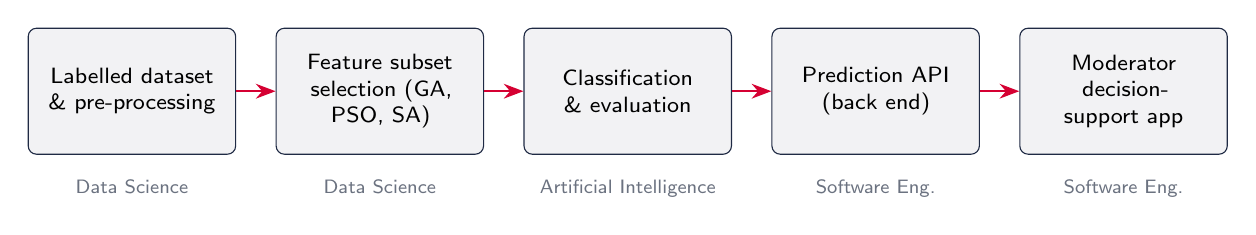
\begin{tikzpicture}[
    node distance=0.5cm,
    box/.style={draw=brandprimary, fill=brandprimary!6, rounded corners=3pt,
                align=center, font=\footnotesize\sffamily, minimum height=1.6cm, text width=2.4cm},
    arrow/.style={-{Stealth[length=2.5mm]}, thick, brandaccent},
    team/.style={font=\scriptsize\sffamily, text=brandmuted}
]
  \node[box] (data)  {Labelled dataset \& pre-processing};
  \node[box, right=of data]  (prep)  {Feature subset selection (GA, PSO, SA)};
  \node[box, right=of prep]  (model) {Classification \& evaluation};
  \node[box, right=of model] (api)   {Prediction API (back end)};
  \node[box, right=of api]   (ui)    {Moderator decision-support app};

  \draw[arrow] (data) -- (prep);
  \draw[arrow] (prep) -- (model);
  \draw[arrow] (model) -- (api);
  \draw[arrow] (api) -- (ui);

  \node[team, below=0.2cm of data]  {Data Science};
  \node[team, below=0.2cm of prep]  {Data Science};
  \node[team, below=0.2cm of model] {Artificial Intelligence};
  \node[team, below=0.2cm of api]   {Software Eng.};
  \node[team, below=0.2cm of ui]    {Software Eng.};
\end{tikzpicture}
\caption{High-level overview of the proposed \projectname{} solution, based on the PRISMO methodology, and the discipline leading each stage}
\label{fig:solution-overview}
\end{figure}

\paragraph{Data.} Collecting live data directly from platforms is increasingly restricted by API access limits and terms of service, and newly collected data would have no reliable ground-truth labels. The project will therefore use publicly available research datasets of \emph{real} social media accounts that have already been labelled as genuine or spam. The preferred dataset is the labelled Twitter spammer dataset used by PRISMO \parencite{benevenuto2010detecting}, which allows the project's results to be compared directly with the paper's. Because this dataset is released on request, the Cresci-2017 social spambot dataset \parencite{cresci2017paradigm} and the TwiBot-20 benchmark \parencite{feng2021twibot20} are kept as fallbacks. Final dataset selection is part of the project scope (Section~\ref{sec:scope}).

\paragraph{Features.} Rather than judging an account on a single post, \projectname{} classifies the \emph{account as a whole} using the categories of signal summarised in Table~\ref{tab:feature-categories}. This account-level approach brings together content analysis (as used in misinformation detection) and pattern-based classification (as used in spam detection).

\begin{table}[htbp]
\centering
\caption{Feature categories used to characterise each account}
\label{tab:feature-categories}
\begin{tabularx}{\textwidth}{@{}>{\bfseries}p{0.2\textwidth} X X@{}}
  \toprule
  Category & \textbf{What it captures} & \textbf{Example features} \\
  \midrule
  Content-based & What the account posts & Hashtags, URLs and mentions per tweet; fraction of tweets containing URLs; character and word counts; retweet statistics \\
  User behaviour & How the account acts and is connected over time & Number of followers and followees, follower-to-followee ratio, total tweets, tweets per day and per week, account age \\
  Profile metadata\textsuperscript{*} & Static information about how the account is set up & Default profile image, description length, digits in username, verified status \\
  \midrule
  \multicolumn{3}{@{}l}{\footnotesize \textsuperscript{*}Available only in the fallback datasets; the PRISMO dataset provides 41 content-based and 21 user-behaviour features.} \\
  \bottomrule
\end{tabularx}
\end{table}

\paragraph{Feature selection.} Not every feature is useful: irrelevant and redundant features can reduce accuracy and increase training time. Following PRISMO, three optimisation algorithms (a Genetic Algorithm, Particle Swarm Optimisation and Simulated Annealing) will each select a feature subset, and these subsets will be combined by priority, keeping the features chosen by at least two of the three algorithms \parencite{agrawal2018prismo}. A smaller feature set also makes the application easier to use, because users only need to provide the selected features. The method is described in more detail in Section~\ref{sec:prismo}.

\paragraph{Models.} As in PRISMO, Random Forest, Na\"ive Bayes, a rule-based learner and a decision tree will be trained on the full feature set and on each selected subset, and their performance will be compared against the objectives in Section~\ref{sec:objectives}. To address the transparency problem, model predictions will be explained using feature-attribution techniques such as SHAP values \parencite{lundberg2017unified}, so that each prediction is accompanied by the factors that influenced it most.

\paragraph{Moderator-centred application.} The trained model will be served through a FastAPI back end and accessed through a React.js front end, designed around how moderators work:

\begin{itemize}[nosep]
  \item \textbf{Reduced input:} a single account is checked by entering only the features kept by feature selection (around a third of the original 62), or by choosing a sample account.
  \item \textbf{Plain-language explanations:} each prediction lists its main reasons, comparing the account's values with those of typical genuine and spam accounts.
  \item \textbf{Confidence and review zone:} predictions close to the decision boundary are labelled \emph{uncertain} and flagged for human review rather than forced into a label.
  \item \textbf{Batch triage:} uploaded accounts are sorted by risk, with uncertain cases highlighted, so that moderators can deal with the most urgent accounts first and export their decisions.
  \item \textbf{Interactive visualisations:} interactive charts show why an individual account was flagged, how risk is distributed across a batch, and how the models and feature sets compare.
\end{itemize}

The design of the application and how it applies recognised usability principles are described in Section~\ref{sec:design}.

\paragraph{User evaluation.} Finally, the tool will be evaluated in a user study in which participants acting as moderators review a set of accounts with and without explanations, and with the reduced and full input forms. The study includes some accounts that the model misclassifies, to test whether explanations help users catch errors (RQ4). Results will be measured through task time, decision accuracy, the System Usability Scale \parencite{brooke1996sus} and a trust questionnaire.

\clearpage
% =====================================================================
%  2. TEAM INTRODUCTION
% =====================================================================
\section{Team Introduction}\label{sec:team}

\subsection{Team Overview}\label{sec:team-overview}
\teamname{} is a team of four students from \institution{} undertaking \projectname{} in \unitcode{} \unitname. The team combines three complementary disciplines, which together cover every stage of the solution shown in Figure~\ref{fig:solution-overview}:

\begin{itemize}[nosep]
  \item \textbf{Data Science} (\memberOne{} and \memberTwo{}) -- leads data preparation, exploratory analysis, feature selection and evaluation;
  \item \textbf{Artificial Intelligence} (\memberFour{}) -- leads model development and designed the front-end prototype; and
  \item \textbf{Software Engineering} (\memberThree{}) -- leads application development and user experience.
\end{itemize}

At the team's first meeting, members shared their strengths and areas to improve. The Data Science and AI members are less familiar with React and FastAPI, while the Software Engineering member has less experience with model training. Work is therefore shared at the boundaries between stages, and members pair up to cover each other's skill gaps, so that no stage depends on a single person.

\subsection{Team Members}\label{sec:team-members}
% ---------------------------------------------------------------------
%  Team member 1
% ---------------------------------------------------------------------
\subsubsection{\memberOne{} -- \memberOneDiscipline}

I am \memberOne{} (student ID \memberOneID), a third-year student majoring in Data Science at \institution. Through my studies I have developed a foundation in Python programming, data wrangling, statistics, databases and machine learning, and I am particularly interested in applying machine learning to real-world problems.

I have co-authored a paper on printed circuit board (PCB) defect detection using machine learning in production, with VietDynamics and partners from Deakin University, Aalto University and Vietnam National University. I have also recently returned from an exchange semester at Swinburne's Hawthorn campus.

In this project I take on two roles. As \textbf{Project Manager}, I am responsible for planning and scheduling the work, coordinating team meetings, tracking progress against the schedule, managing risks and change requests, and acting as the main point of contact with our tutor. My aim is to keep the team aligned and to make sure each discipline's work fits together into a single, working product. As \textbf{Data Engineering Lead}, I will source the labelled account datasets and build the data cleaning and pre-processing pipeline that underpins all later feature engineering and modelling.

Through this project I hope to strengthen my project management, communication and applied machine learning skills, and to gain hands-on experience delivering a complete data-driven product from raw data through to a usable application.

% ---------------------------------------------------------------------
%  Team member 2 
% ---------------------------------------------------------------------
\subsubsection{\memberTwo{} -- \memberTwoDiscipline}
{I am Nguyen Minh Vo (student ID 105505636), a second-year undergraduate student majoring in Data Science at Swinburne University of Technology. Through my university coursework, I have acquired foundational knowledge in Python programming, statistical analysis, and data manipulation. I have a keen interest in exploratory data analysis and understanding how machine learning models make decisions on complex datasets.

In the SpamSentinel project, I serve as the \textbf{Data Analysis and Evaluation Lead}. My primary responsibilities include conducting exploratory data analysis (EDA) to examine feature distributions and address class imbalance in social media datasets. I will also contribute to the feature selection phase by implementing the Particle Swarm Optimisation (PSO) algorithm and combining selected features into the final priority subset. Furthermore, I am responsible for benchmarking classifier performance across evaluation metrics such as macro F1-score and recall, as well as designing interactive data visualisations to help moderators interpret results effectively.

Through this project, I aim to enhance my hands-on skills in data pre-processing and model evaluation workflows, while gaining valuable experience in collaborative project management within a technical environment.}
% ---------------------------------------------------------------------
%  Team member 3
% ---------------------------------------------------------------------
\subsubsection{\memberThree{} -- \memberThreeDiscipline}
{I am Hai Dang Nguyen (student ID 105304590), a second-year undergraduate student majoring in Software Engineering at Swinburne University of Technology. I have a range of development skills, including programming in languages such as Python and Java, an understanding of data structures and algorithms, working with databases, and using version control tools such as Git. Beyond coding, I bring problem-solving, teamwork and communication skills, which help me collaborate effectively and design scalable solutions.

In the SpamSentinel project, I serve as the \textbf{Software and Front-end Lead}. My primary responsibilities include designing and developing the application's user interface and user experience to ensure it is intuitive, efficient and visually appealing. I will create wireframes and mockups to illustrate the app's layout and functionality, while collaborating closely with the team to align design choices with technical feasibility. I will also focus on usability testing, accessibility standards and responsive design principles, so that the app works seamlessly across different devices. By combining creativity with technical knowledge, I aim to deliver a design that enhances user engagement and supports the project's core functionality.

Through this project, I aim to strengthen my software development skills for my major, gain experience in bringing the stages of a project together, and improve my teamwork skills.}

% ---------------------------------------------------------------------
%  Team member 4
% ---------------------------------------------------------------------
\subsubsection{\memberFour{} -- \memberFourDiscipline}

I am \memberFour{}{} (student ID: \memberFourID), a third-year student studying Computer Science with a major in Artificial Intelligence at \institution. I am particularly interested in the process of developing and evaluating AI models, as well as translating their capabilities into practical products that are accessible and useful to users.

In this project, I take on the role of \textbf{Machine Learning Lead}, with responsibilities for training machine learning models and developing the product prototype. For model development, I will investigate suitable approaches, train and compare candidate models, and evaluate their performance against the project requirements. Alongside model development, I will create a product prototype with a professional and user-friendly interface that demonstrates the project's core features. The prototype will also provide a practical basis for demonstrating the AI model's functionality and gathering feedback on the overall user experience. I will collaborate with my teammates to align the interface and model integration with the project's objectives and refine the prototype as development progresses.

Through this project, I hope to strengthen my technical skills in AI model training, evaluation, and product prototyping. I also aim to improve my teamwork and communication skills by clearly explaining technical decisions, coordinating my work with other team members, and responding constructively to feedback. My overall goal is to contribute to a high-quality solution that combines a well-performing, appropriate AI model with a professional prototype, while demonstrating the effective application of our knowledge and a professional approach to development and presentation.


\clearpage
% =====================================================================
%  3. PROJECT REQUIREMENTS
% =====================================================================
\section{Project Requirements}\label{sec:requirements}

% MoSCoW priority labels used in the requirement tables
\newcommand{\must}{\textcolor{brandaccent}{\textbf{Must}}}
\newcommand{\should}{\textcolor{brandprimary}{\textbf{Should}}}
\newcommand{\could}{\textcolor{brandmuted}{\textbf{Could}}}
\newcommand{\reqgroup}[1]{\multicolumn{4}{@{}l}{\cellcolor{brandprimary!8}\textbf{\sffamily #1}} \\}

This section identifies the project's stakeholders and lists the functional and non-functional requirements that \projectname{} must satisfy. Requirements are derived from the objectives in Section~\ref{sec:objectives} and from the methodology of the PRISMO spam detection model \parencite{agrawal2018prismo}, which this project adopts as its primary methodological reference.

\subsection{Stakeholders}\label{sec:stakeholders}

Table~\ref{tab:stakeholders} lists the stakeholders who will use, assess or be affected by \projectname{}, along with their key needs.

\begin{table}[htbp]
\centering
\caption{Project stakeholders and their key needs}
\label{tab:stakeholders}
\begin{tabularx}{\textwidth}{@{}>{\raggedright\arraybackslash}p{0.25\textwidth} >{\raggedright\arraybackslash}p{0.2\textwidth} X@{}}
  \toprule
  \textbf{Stakeholder} & \textbf{Type} & \textbf{Key Needs} \\
  \midrule
  Unit tutor (\supervisor) & Assessor and client & A well-planned project delivered on time that meets the unit's learning outcomes and assessment criteria. \\
  \addlinespace
  Platform moderators and trust \& safety analysts & Primary end users & Fast, accurate identification of suspicious accounts, with clear reasons they can rely on when deciding what action to take. \\
  \addlinespace
  Researchers and data analysts & Secondary end users & Access to model performance, feature selection results and global feature importance to understand how spam accounts behave. \\
  \addlinespace
  Social media users & Indirect beneficiaries & Fewer encounters with spam, scams and misleading content. \\
  \addlinespace
  User study participants & Evaluators & Clear instructions, informed consent, anonymity, and a session of reasonable length. \\
  \addlinespace
  Project team & Developers & Clear, stable and testable requirements; achievable scope within the semester. \\
  \bottomrule
\end{tabularx}
\end{table}

\subsection{Methodological Basis: the PRISMO Model}\label{sec:prismo}

\textcite{agrawal2018prismo} proposed PRISMO (\emph{PRIority based Spam detection using Multi Optimization}), a spam detection approach organised into three phases: \emph{data collection}, \emph{feature subset selection} and \emph{classification}. Its key idea is that many features in spam datasets are irrelevant or redundant, which lowers classifier accuracy and increases training time. PRISMO therefore uses a two-layer hybrid feature selection process:

\begin{enumerate}[nosep]
  \item \textbf{Layer 1 (feature selection):} three metaheuristic optimisation algorithms -- a Genetic Algorithm (GA), Particle Swarm Optimisation (PSO) and Simulated Annealing (SA) -- each independently select a feature subset (FS1, FS2 and FS3).
  \item \textbf{Layer 2 (feature formation):} features selected by all three algorithms are given \emph{priority~1}, features selected by any two are given \emph{priority~2}, and the union of these forms the final subset (FS4). Features selected by only one algorithm are discarded.
\end{enumerate}

Each subset, along with the full feature set as a baseline, was then evaluated with four classifiers (Random Forest, Na\"ive Bayes, JRip and J48) using 10-fold cross-validation. On a labelled Twitter spammer dataset with 62 content and user-behaviour features \parencite{benevenuto2010detecting}, PRISMO reduced the feature set to 19 features while achieving 88.26\% accuracy, a true positive rate (TPR) of 72.4\% and a true negative rate (TNR) of 96.2\% with Random Forest, which was the best-performing classifier across all subsets. Feature reduction also halved model build time, from 1,240\,ms to 620\,ms \parencite{agrawal2018prismo}.

\paragraph{Replication approach.} The team will reproduce PRISMO's \emph{method} rather than attempt to match its exact numbers, for three reasons. First, the paper does not report the parameters of its optimisation algorithms (such as population size, mutation and crossover rates, number of particles, iterations or the annealing schedule), nor the fitness function used to score candidate feature subsets. Second, the description of how the best features from Layer~1 are carried into Layer~2 can be interpreted in more than one way. Third, GA, PSO and SA are stochastic, so results vary between runs even with identical settings. The team will therefore document every parameter and interpretation it adopts (NFR9) and compare its results against the ranges reported in the paper. The feature subsets PRISMO selected, which the paper lists in full, provide an additional check on the implementation.

It is also worth noting that, in PRISMO's own results, the differences in accuracy between feature sets are small: with Random Forest, the full feature set achieved 88.16\%, PRISMO 88.26\% and GA alone 88.73\% \parencite{agrawal2018prismo}. PRISMO's main benefit is therefore that it cuts the number of features by roughly two-thirds and halves model build time \emph{without losing accuracy}, rather than that it increases accuracy. This project will test whether the same holds in its own experiments.

\projectname{} follows PRISMO's three-phase methodology and extends it to address its limitations and this project's objectives, as summarised in Table~\ref{tab:prismo-alignment}.

% Not a floating table, so that it keeps its number before the long requirement tables that follow
\begin{center}
\captionof{table}{How \projectname{} adopts and extends the PRISMO methodology}
\label{tab:prismo-alignment}
\begin{tabularx}{\textwidth}{@{}>{\raggedright\arraybackslash}p{0.17\textwidth} >{\raggedright\arraybackslash}X >{\raggedright\arraybackslash}X >{\raggedright\arraybackslash}p{0.11\textwidth}@{}}
  \toprule
  \textbf{Phase} & \textbf{PRISMO \parencite{agrawal2018prismo}} & \textbf{\projectname{}} & \textbf{Req.} \\
  \midrule
  Data collection & Labelled Twitter spammer dataset with 62 content and user-behaviour features & Same dataset where access is granted, with an alternative public dataset as a fallback & FR1--FR3 \\
  \addlinespace
  Feature subset selection & GA, PSO and SA (Layer 1) combined by priority rules (Layer 2), implemented in MATLAB & Same two-layer process re-implemented in Python, with fixed random seeds and documented parameters for reproducibility & FR4--FR6, NFR9 \\
  \addlinespace
  Classification & Random Forest, Na\"ive Bayes, JRip and J48 in WEKA, 10-fold cross-validation & Equivalent classifiers in Python, plus an optional gradient-boosting model; 10-fold cross-validation \emph{and} a held-out test set & FR7--FR8 \\
  \addlinespace
  Evaluation & Accuracy, TPR, TNR and model build time & Adds precision, F1-score and ROC-AUC, with a focus on improving spammer detection (TPR) & FR9, NFR1 \\
  \addlinespace
  \emph{Extension} & Not addressed; evaluation is limited to model metrics & Moderator-centred decision support (plain-language explanations, review zone, batch triage, reduced input form), evaluated through a user study & FR11--FR23, NFR12 \\
  \bottomrule
\end{tabularx}
\end{center}

\subsection{Functional Requirements}\label{sec:functional-req}

Requirements are prioritised using the MoSCoW method: \must{} (essential for the project to succeed), \should{} (important but not essential), and \could{} (desirable if time permits). Together, the \must{} requirements form the project's \textbf{core scope}, which reproduces the PRISMO pipeline end to end and makes it usable through the web application. The \should{} and \could{} requirements form the \textbf{stretch scope}, which is delivered only once the core is complete and stable. Items the team has explicitly decided not to deliver are recorded as out of scope in Section~\ref{sec:scope}.

{\renewcommand{\arraystretch}{1.25}
\begin{longtable}{@{}>{\raggedright\arraybackslash}p{0.07\textwidth} >{\raggedright\arraybackslash}p{0.21\textwidth} >{\raggedright\arraybackslash}p{0.52\textwidth} >{\raggedright\arraybackslash}p{0.09\textwidth}@{}}
  \caption{Functional requirements}\label{tab:functional-req} \\
  \toprule
  \textbf{ID} & \textbf{Requirement} & \textbf{Description} & \textbf{Priority} \\
  \midrule
  \endfirsthead
  \multicolumn{4}{@{}l}{\small\itshape Table~\thetable{} continued} \\
  \toprule
  \textbf{ID} & \textbf{Requirement} & \textbf{Description} & \textbf{Priority} \\
  \midrule
  \endhead
  \bottomrule
  \endlastfoot

  \reqgroup{Phase 1 -- Data Collection and Preparation}
  FR1 & Dataset acquisition & Obtain at least one labelled dataset of real social media accounts. The Twitter spammer dataset used by PRISMO \parencite{benevenuto2010detecting} is preferred and was requested from its authors on Monday 5 October. If access has not been granted within one week (by Monday 12 October), the team will switch to Cresci-2017 \parencite{cresci2017paradigm} or TwiBot-20 \parencite{feng2021twibot20}. & \must \\
  FR2 & Data pre-processing & Clean the data (missing values, duplicates, invalid records), scale numerical features, assess class imbalance, and create stratified training and test splits. & \must \\
  FR3 & Feature preparation & Map the dataset's features into the content-based, user-behaviour and profile categories in Table~\ref{tab:feature-categories}. The PRISMO dataset already provides its 62 features. If a fallback dataset is used, compute equivalent features from the raw account and tweet data following the definitions of \textcite{benevenuto2010detecting}. & \must \\

  \reqgroup{Phase 2 -- Feature Subset Selection}
  FR4 & Baseline feature set & Train and evaluate all classifiers on the full feature set, without selection, as the comparison baseline. & \must \\
  FR5 & Metaheuristic feature selection & Implement GA, PSO and SA feature selection to produce subsets FS1, FS2 and FS3 (PRISMO Layer 1). & \must \\
  FR6 & Priority-based feature formation & Combine FS1--FS3 into FS4 using PRISMO's priority rules: keep features selected by all three (priority~1) or any two (priority~2) algorithms, and discard the rest (PRISMO Layer 2). & \must \\

  \reqgroup{Phase 3 -- Classification and Evaluation}
  FR7 & Multi-classifier training & Train Random Forest, Na\"ive Bayes, a rule-based learner (RIPPER, equivalent to JRip) and a decision tree (equivalent to J48) on each feature set. A gradient-boosting model may be added for comparison. & \must \\
  FR8 & Model validation & Validate every feature-set and classifier combination using stratified 10-fold cross-validation, and confirm the final model on the held-out test set. & \must \\
  FR9 & Performance comparison & Report accuracy, TPR (recall), TNR (specificity), precision, F1-score, ROC-AUC and model build time for every combination, in comparison tables and charts. & \must \\
  FR10 & Model export & Save the selected model and its pre-processing and feature-selection pipeline so that the back end can load it. & \must \\

  \reqgroup{Explainability and Decision Support}
  FR11 & Per-prediction explanation & For each prediction, compute the features that contributed most to the result (e.g.\ using SHAP values \parencite{lundberg2017unified}). & \must \\
  FR12 & Plain-language explanations & Present the top contributing features as short, plain-language statements that compare the account's value with typical values for genuine and spam accounts in the training data. & \must \\
  FR13 & Uncertainty review zone & Label predictions whose confidence falls within a defined band around the decision threshold as \emph{uncertain -- review recommended}, rather than as genuine or spam. & \must \\
  FR14 & Global feature insights & Show overall feature importance and which features each selection algorithm chose. & \should \\

  \reqgroup{Web Application}
  FR15 & Single account check & Allow a user to enter the values of the \emph{selected} features only (FS4, rather than all 62), or choose a sample account from the dataset, and receive a label with a confidence score and explanation. & \must \\
  FR16 & Batch triage queue & Allow a user to upload a CSV file of accounts and view the predictions as a queue sorted by risk, with uncertain cases highlighted, filtering options, and export of results and the user's decisions. & \must \\
  FR17 & Prediction API & Provide FastAPI back-end endpoints, using at least the GET and POST methods, for single prediction, batch prediction, explanations, model metrics and feature information. & \must \\
  FR18 & Input validation and error handling & Validate user input in the React front end before it is sent, and again in the back end. Handle all errors gracefully, with clear, specific messages explaining how to fix problems. & \must \\
  FR19 & Interactive visualisations & Present results through at least three types of interactive chart (e.g.\ a per-prediction explanation chart, the risk distribution of a batch, and model and feature-set comparisons from FR9), supporting hover details, zooming or filtering, and export as images. & \must \\
  FR20 & Help and about page & Explain how \projectname{} works, what the confidence score and review zone mean, and the model's limitations. & \could \\
  FR21 & Moderator feedback & Allow a user to mark that they disagree with a prediction, and include these disagreements in the exported results for future retraining. & \could \\

  \reqgroup{User Evaluation}
  FR22 & Study mode & Provide a study configuration in which explanations can be switched on or off, and the reduced (FS4) or full (62-feature) input form can be selected, so that conditions can be compared. & \must \\
  FR23 & Interaction logging & In study mode, anonymously record each participant's decisions, task completion times and input errors, and export them as CSV for analysis. & \must \\
\end{longtable}
}

\subsection{Non-Functional Requirements}\label{sec:nonfunctional-req}

{\renewcommand{\arraystretch}{1.25}
\begin{longtable}{@{}>{\raggedright\arraybackslash}p{0.07\textwidth} >{\raggedright\arraybackslash}p{0.21\textwidth} >{\raggedright\arraybackslash}p{0.52\textwidth} >{\raggedright\arraybackslash}p{0.09\textwidth}@{}}
  \caption{Non-functional requirements}\label{tab:nonfunctional-req} \\
  \toprule
  \textbf{ID} & \textbf{Requirement} & \textbf{Description} & \textbf{Priority} \\
  \midrule
  \endfirsthead
  \multicolumn{4}{@{}l}{\small\itshape Table~\thetable{} continued} \\
  \toprule
  \textbf{ID} & \textbf{Requirement} & \textbf{Description} & \textbf{Priority} \\
  \midrule
  \endhead
  \bottomrule
  \endlastfoot

  NFR1 & Detection performance & The selected model must achieve a macro-averaged F1-score of at least 0.85 on the held-out test set (Objective O4). Its spammer detection rate (TPR) should exceed PRISMO's 72.4\%, because a missed spam account is more harmful than a false alarm. & \must \\
  NFR2 & Efficiency & Feature selection must reduce model build time compared with the full feature set, as demonstrated by PRISMO. & \should \\
  NFR3 & Response time & A single prediction must be returned within 2 seconds, and a batch of 1,000 accounts within 30 seconds, on a standard laptop. & \must \\
  NFR4 & Usability & The interface must follow recognised usability heuristics \parencite{nielsen1994heuristics}. A first-time user should be able to complete a single account check within one minute without instructions, and the application should score at least 68 on the System Usability Scale \parencite{brooke1996sus} in user testing. & \must \\
  NFR5 & Transparency & Every prediction must be shown with its confidence score and its top contributing features in plain language. & \must \\
  NFR6 & Accessibility & The interface should meet WCAG 2.1 Level AA colour-contrast and keyboard-navigation guidelines \parencite{w3c2018wcag21}. & \should \\
  NFR7 & Compatibility and responsiveness & The application must work on current versions of Chrome, Firefox and Edge, with a responsive layout for desktop, tablet and mobile screen sizes. & \must \\
  NFR8 & Security & Uploaded files must be checked for type (CSV only) and size (maximum 5\,MB), parsed as data only, and never executed. & \must \\
  NFR9 & Reproducibility & Because GA, PSO and SA are stochastic and sensitive to their parameters \parencite{agrawal2018prismo}, all experiments must use fixed random seeds and record their parameters (e.g.\ population size, mutation and crossover rates, number of particles). Any interpretation of steps the paper does not fully specify must be documented. & \must \\
  NFR10 & Privacy and ethics & Only publicly available research datasets may be used, in line with their terms of use. Uploaded data must be processed in memory and not stored after the session. & \must \\
  NFR11 & Maintainability & Code must be modular, version-controlled on GitHub, peer-reviewed before merging, and documented with a README covering set-up and usage. & \must \\
  NFR12 & Research ethics & The user study must follow Swinburne's requirements for research involving people, including obtaining any required approval before sessions begin. Participation must be voluntary and based on informed consent, participants may withdraw at any time, and all study data must be anonymous. & \must \\
\end{longtable}
}

\subsection{Requirements Traceability}\label{sec:traceability}

Table~\ref{tab:traceability} maps each project objective and research question to the requirements that deliver it, so that every objective is covered and every requirement has a clear purpose.

\begin{table}[htbp]
\centering
\caption{Traceability between objectives, research questions and requirements}
\label{tab:traceability}
\begin{tabularx}{\textwidth}{@{}>{\raggedright\arraybackslash}p{0.38\textwidth} X@{}}
  \toprule
  \textbf{Objective / Research Question} & \textbf{Requirements} \\
  \midrule
  O1 -- Data acquisition and preparation & FR1, FR2, NFR10 \\
  O2 -- Feature engineering and selection & FR3, FR4, FR5, FR6, NFR9 \\
  O3 -- Model development                & FR7, FR10, NFR2 \\
  O4 -- Evaluation                       & FR8, FR9, NFR1 \\
  O5 -- Explainability and decision support & FR11--FR14, NFR5 \\
  O6 -- Web application                  & FR15--FR21, NFR3, NFR4, NFR6, NFR7, NFR8 \\
  O7 -- User evaluation                  & FR22, FR23, NFR4, NFR12 \\
  O8 -- Project management               & NFR11; Sections~\ref{sec:scope}--\ref{sec:closure} \\
  \midrule
  RQ1 -- Reproducing PRISMO              & FR4--FR9, NFR1, NFR9 \\
  RQ2 -- Effect of feature selection on use & FR15, FR22, FR23 \\
  RQ3, RQ4 -- Effect of explanations     & FR11--FR13, FR22, FR23 \\
  RQ5 -- Usability and trust             & NFR4, FR23 \\
  \bottomrule
\end{tabularx}
\end{table}

\clearpage
% =====================================================================
%  4. SCOPE MANAGEMENT
% =====================================================================
\section{Scope Management}\label{sec:scope}

Scope management defines and controls what is, and is not, included in the project, so that the team delivers everything required and nothing that is not \parencite{pmi2021pmbok}. This section presents the project scope statement, the assumptions and constraints that shape it, the Work Breakdown Structure (WBS) and the WBS dictionary.

\subsection{Project Scope Statement}\label{sec:scope-statement}

\paragraph{Scope description.} The project will reproduce the PRISMO spam detection methodology \parencite{agrawal2018prismo} on a labelled dataset of real social media accounts, and deliver the resulting model through \projectname{}, a moderator-centred web application that lets users check individual accounts or triage batches of accounts, see in plain language why each account was classified as genuine or spam, and identify uncertain cases that need human review. The tool will then be evaluated in a user study to answer research questions RQ2--RQ5 (Section~\ref{sec:rqs}). Work covers the full life cycle, from dataset acquisition and feature selection through classification, evaluation and application development, to user evaluation and closure.

\paragraph{Core and stretch scope.} Following the prioritisation in Section~\ref{sec:requirements}, the scope is divided into two tiers:

\begin{itemize}[nosep]
  \item \textbf{Core scope} (all \textbf{Must} requirements): the complete PRISMO pipeline (data preparation, GA, PSO and SA feature selection, priority-based feature formation, four classifiers and 10-fold cross-validation), the FastAPI back end, the React front end with its decision-support features (plain-language explanations, uncertainty review zone, reduced-input single-account check and batch triage queue), at least three types of interactive chart, study mode, testing, and the user study.
  \item \textbf{Stretch scope} (\textbf{Should} and \textbf{Could} requirements): global feature insights, an additional gradient-boosting classifier, the help page and moderator feedback. Stretch items begin only once the core scope is complete and stable.
\end{itemize}

\paragraph{Project deliverables.} Table~\ref{tab:deliverables} lists the deliverables the project will produce, grouped by the assessment in which each is submitted.

\begin{table}[htbp]
\centering
\caption{Project deliverables and due dates}
\label{tab:deliverables}
\begin{tabularx}{\textwidth}{@{}l >{\raggedright\arraybackslash}p{0.24\textwidth} >{\raggedright\arraybackslash}X >{\raggedright\arraybackslash}p{0.13\textwidth} l@{}}
  \toprule
  \textbf{ID} & \textbf{Deliverable} & \textbf{Description} & \textbf{Due} & \textbf{WBS} \\
  \midrule
  D1 & Project Management Plan & This document, including the initial front-end prototype & A1, Sun 11 Oct & 1.1, 5.2 \\
  \midrule
  D2 & Processed datasets & Cleaned, pre-processed datasets and selected feature subsets (CSV/JSON) & A2, Mon 2 Nov & 2, 3 \\
  D3 & Model source code and final models & Python implementation of pre-processing, GA, PSO, SA, priority-based feature formation and classifiers, with the exported final model & A2, Mon 2 Nov & 3, 4 \\
  D4 & AI model report and README & Report of up to 3,000 words (PDF) presenting methods, results and the comparison with PRISMO (RQ1); README explaining how to run the code & A2, Mon 2 Nov & 4.3, 7.1 \\
  \midrule
  D5 & Web application source code & React front end, FastAPI back end with the integrated model, and a README covering set-up and configuration & A3, Sun 6 Dec & 4.4, 5, 6.1 \\
  D6 & User study results & Study protocol, ethics documentation, anonymised results and analysis answering RQ2--RQ5, included in the Assignment~3 report & A3, Sun 6 Dec & 6.3, 6.4 \\
  D7 & Web application report & Report (PDF) covering architecture, implementation, API documentation, model integration and conclusions & A3, Sun 6 Dec & 7.2 \\
  D8 & Demonstration video & Video of up to 7 minutes (MP4) showing all functionality and responsiveness on desktop, tablet and mobile & A3, Sun 6 Dec & 7.3 \\
  \midrule
  D9 & Lessons learned record & Retrospective findings and final, archived repository & Tue 8 Dec & 7.4 \\
  \bottomrule
\end{tabularx}
\end{table}

\paragraph{In scope and out of scope.} Table~\ref{tab:in-out-scope} sets clear boundaries for the project. Any request to move an item from out of scope to in scope must go through the change control process (Section~\ref{sec:change-control}).

\begin{table}[htbp]
\centering
\caption{In-scope and out-of-scope items}
\label{tab:in-out-scope}
\begin{tabularx}{\textwidth}{@{}>{\raggedright\arraybackslash}X >{\raggedright\arraybackslash}X@{}}
  \toprule
  \textbf{In scope} & \textbf{Out of scope} \\
  \midrule
  \begin{itemize}[nosep, leftmargin=*, label={\color{brandprimary}\textbullet}]
    \item Account-level spam classification using public, labelled research datasets
    \item Reproducing PRISMO's method (feature selection and classification)
    \item Comparing results against the ranges reported by PRISMO
    \item Python implementation of all algorithms
    \item Prediction API and web application for single and batch checks
    \item Plain-language explanations, uncertainty review zone and batch triage
    \item User study with student participants acting as moderators
    \item Functional, performance and usability testing
    \item React.js front end with at least three interactive chart types, and FastAPI back end
  \end{itemize}
  &
  \begin{itemize}[nosep, leftmargin=*, label={\color{brandaccent}\textbullet}]
    \item Collecting live data from social media platforms or their APIs
    \item Real-time monitoring of platforms, or automatically suspending accounts
    \item Matching PRISMO's exact reported numbers
    \item Studies with real platform moderators
    \item Post-level fact-checking or misinformation verification
    \item Analysis of images, video, or non-English content
    \item User registration (sign-up) and stored user accounts or personal data
    \item Production-scale cloud deployment, and native mobile apps (mobile users are supported through the responsive web application)
  \end{itemize}
  \\
  \bottomrule
\end{tabularx}
\end{table}

\subsection{Assumptions and Constraints}\label{sec:assumptions}

\paragraph{Assumptions.} The plan is based on the following assumptions. If any proves false, it will be treated as a risk (Section~\ref{sec:risk}) or a change request (Section~\ref{sec:change-control}).

\begin{enumerate}[label=\textbf{A\arabic*}, leftmargin=2.5em, nosep]
  \item Access to the PRISMO dataset will be granted within one week of the request; otherwise, a fallback dataset (Cresci-2017 or TwiBot-20) is suitable.
  \item Each team member can contribute about 12 hours per week throughout the project.
  \item Team members' laptops are powerful enough to run all experiments; no GPU or paid cloud computing is required.
  \item The free, open-source Python libraries the project depends on (e.g.\ for machine learning, optimisation and web development) are available and stable.
  \item The tutor is available for regular consultation and feedback.
  \item Any ethics approval required for the user study can be obtained before the study is scheduled to begin, and 8--12 participants can be recruited.
\end{enumerate}

\paragraph{Constraints.}

\begin{enumerate}[label=\textbf{C\arabic*}, leftmargin=2.5em, nosep]
  \item \textbf{Time:} the project runs for about eleven and a half weeks, from the kick-off meeting on 20 September to 8 December 2026, with fixed assessment deadlines on 11 October, 2 November and 6 December (Section~\ref{sec:time}).
  \item \textbf{Technology:} the unit requires a React.js front end and a FastAPI back end, with at least two HTTP methods and at least two chart types (three interactive chart types for a High Distinction).
  \item \textbf{Budget:} there is no project budget; only free and open-source tools, and free tiers of any services, may be used.
  \item \textbf{People:} the team has four members. Application development is led by the Software Engineering member, but the Project Manager also has full-stack development skills and the other members can support application tasks when needed.
  \item \textbf{Data:} the project is limited to publicly available, pre-labelled research datasets. The PRISMO dataset was collected in 2009 and provides only pre-computed features, so the trained model is a proof of concept and may not reflect current spammer behaviour.
  \item \textbf{Method:} PRISMO does not report its optimisation parameters or fitness function, so the team must make and document its own choices (NFR9).
  \item \textbf{Participants:} the user study relies on students acting as moderators rather than professional moderators, which limits how far its results can be generalised.
\end{enumerate}

\subsection{Work Breakdown Structure}\label{sec:wbs}

The WBS breaks the total scope of the project into smaller, manageable work packages \parencite{pmi2021pmbok}. It is deliverable-oriented and follows PRISMO's three phases (WBS 2--4), with packages for project management, moderator-centred application development, integration, testing and user evaluation, and closure around them (Figure~\ref{fig:wbs}). Together, the work packages cover all of the project's scope, and nothing outside it. No work package is stretch scope in its entirety; stretch requirements are delivered within the relevant packages (for example, global feature insights in 4.4 and the help page in 5.4).

\begin{landscape}
\begin{figure}[p]
\centering
\resizebox{\linewidth}{!}{% =====================================================================
%  WBS diagram -- generated; edit the labels here or regenerate
% =====================================================================
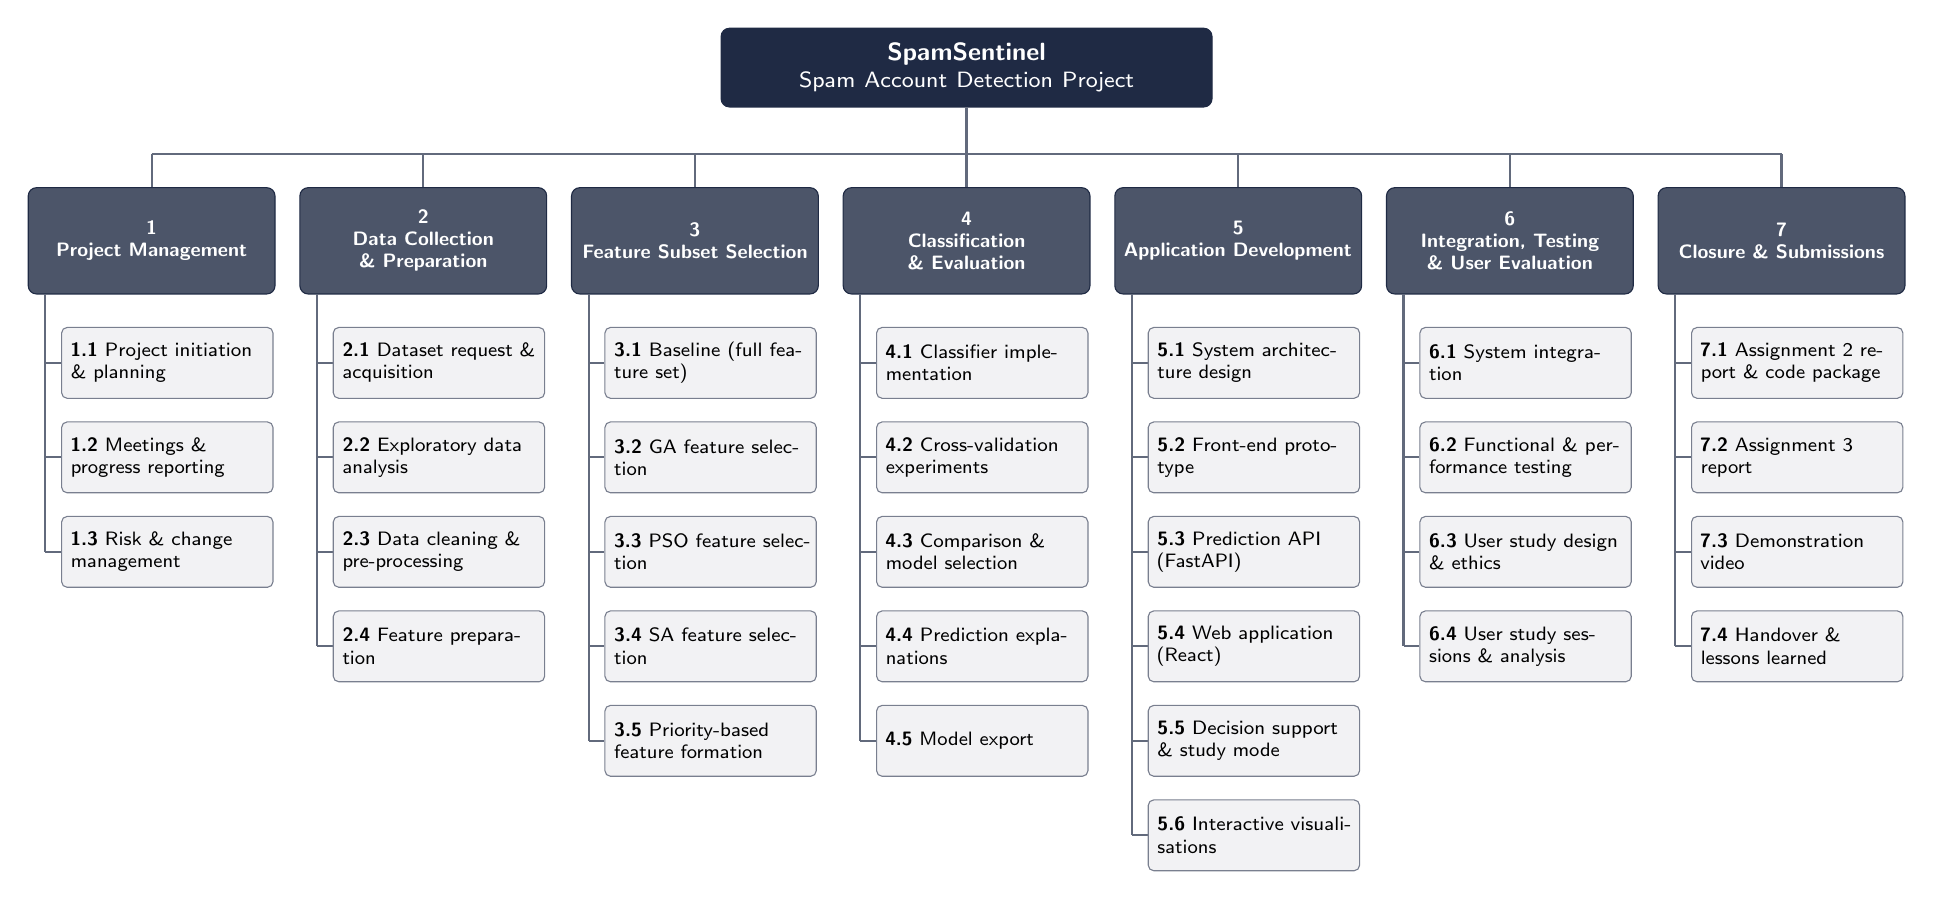
\begin{tikzpicture}[
    root/.style={draw=brandprimary, fill=brandprimary, text=white, rounded corners=3pt,
                 font=\small\sffamily\bfseries, align=center, minimum height=1cm, text width=6cm},
    lvl2/.style={draw=brandprimary, fill=brandprimary!80, text=white, rounded corners=3pt,
                 font=\scriptsize\sffamily\bfseries, align=center, minimum height=1.35cm, text width=2.9cm},
    lvl3/.style={draw=brandprimary!60, fill=brandprimary!6, rounded corners=2pt,
                 font=\scriptsize\sffamily, align=left, minimum height=0.9cm, text width=2.45cm,
                 anchor=west},
    link/.style={draw=brandprimary!70, thick}
]
  \node[root] (root) at (0,0) {\projectname{}\\[-1pt]{\footnotesize\mdseries Spam Account Detection Project}};
  \draw[link] (root.south) -- (0,-1.1);
  \draw[link] (-10.35,-1.1) -- (10.35,-1.1);
  \draw[link] (-10.35,-1.1) -- (-10.35,-1.53);
  \node[lvl2] (n1) at (-10.35,-2.20) {1\\Project Management};
  \draw[link] (-11.70,-2.88) -- (-11.70,-6.15);
  \draw[link] (-11.70,-3.75) -- (-11.50,-3.75);
  \node[lvl3] at (-11.50,-3.75) {\textbf{1.1} Project initiation \& planning};
  \draw[link] (-11.70,-4.95) -- (-11.50,-4.95);
  \node[lvl3] at (-11.50,-4.95) {\textbf{1.2} Meetings \& progress reporting};
  \draw[link] (-11.70,-6.15) -- (-11.50,-6.15);
  \node[lvl3] at (-11.50,-6.15) {\textbf{1.3} Risk \& change management};
  \draw[link] (-6.90,-1.1) -- (-6.90,-1.53);
  \node[lvl2] (n2) at (-6.90,-2.20) {2\\Data Collection \& Preparation};
  \draw[link] (-8.25,-2.88) -- (-8.25,-7.35);
  \draw[link] (-8.25,-3.75) -- (-8.05,-3.75);
  \node[lvl3] at (-8.05,-3.75) {\textbf{2.1} Dataset request \& acquisition};
  \draw[link] (-8.25,-4.95) -- (-8.05,-4.95);
  \node[lvl3] at (-8.05,-4.95) {\textbf{2.2} Exploratory data analysis};
  \draw[link] (-8.25,-6.15) -- (-8.05,-6.15);
  \node[lvl3] at (-8.05,-6.15) {\textbf{2.3} Data cleaning \& pre-processing};
  \draw[link] (-8.25,-7.35) -- (-8.05,-7.35);
  \node[lvl3] at (-8.05,-7.35) {\textbf{2.4} Feature preparation};
  \draw[link] (-3.45,-1.1) -- (-3.45,-1.53);
  \node[lvl2] (n3) at (-3.45,-2.20) {3\\Feature Subset Selection};
  \draw[link] (-4.80,-2.88) -- (-4.80,-8.55);
  \draw[link] (-4.80,-3.75) -- (-4.60,-3.75);
  \node[lvl3] at (-4.60,-3.75) {\textbf{3.1} Baseline (full feature set)};
  \draw[link] (-4.80,-4.95) -- (-4.60,-4.95);
  \node[lvl3] at (-4.60,-4.95) {\textbf{3.2} GA feature selection};
  \draw[link] (-4.80,-6.15) -- (-4.60,-6.15);
  \node[lvl3] at (-4.60,-6.15) {\textbf{3.3} PSO feature selection};
  \draw[link] (-4.80,-7.35) -- (-4.60,-7.35);
  \node[lvl3] at (-4.60,-7.35) {\textbf{3.4} SA feature selection};
  \draw[link] (-4.80,-8.55) -- (-4.60,-8.55);
  \node[lvl3] at (-4.60,-8.55) {\textbf{3.5} Priority-based feature formation};
  \draw[link] (0.00,-1.1) -- (0.00,-1.53);
  \node[lvl2] (n4) at (0.00,-2.20) {4\\Classification \& Evaluation};
  \draw[link] (-1.35,-2.88) -- (-1.35,-8.55);
  \draw[link] (-1.35,-3.75) -- (-1.15,-3.75);
  \node[lvl3] at (-1.15,-3.75) {\textbf{4.1} Classifier implementation};
  \draw[link] (-1.35,-4.95) -- (-1.15,-4.95);
  \node[lvl3] at (-1.15,-4.95) {\textbf{4.2} Cross-validation experiments};
  \draw[link] (-1.35,-6.15) -- (-1.15,-6.15);
  \node[lvl3] at (-1.15,-6.15) {\textbf{4.3} Comparison \& model selection};
  \draw[link] (-1.35,-7.35) -- (-1.15,-7.35);
  \node[lvl3] at (-1.15,-7.35) {\textbf{4.4} Prediction explanations};
  \draw[link] (-1.35,-8.55) -- (-1.15,-8.55);
  \node[lvl3] at (-1.15,-8.55) {\textbf{4.5} Model export};
  \draw[link] (3.45,-1.1) -- (3.45,-1.53);
  \node[lvl2] (n5) at (3.45,-2.20) {5\\Application Development};
  \draw[link] (2.10,-2.88) -- (2.10,-9.75);
  \draw[link] (2.10,-3.75) -- (2.30,-3.75);
  \node[lvl3] at (2.30,-3.75) {\textbf{5.1} System architecture design};
  \draw[link] (2.10,-4.95) -- (2.30,-4.95);
  \node[lvl3] at (2.30,-4.95) {\textbf{5.2} Front-end prototype};
  \draw[link] (2.10,-6.15) -- (2.30,-6.15);
  \node[lvl3] at (2.30,-6.15) {\textbf{5.3} Prediction API (FastAPI)};
  \draw[link] (2.10,-7.35) -- (2.30,-7.35);
  \node[lvl3] at (2.30,-7.35) {\textbf{5.4} Web application (React)};
  \draw[link] (2.10,-8.55) -- (2.30,-8.55);
  \node[lvl3] at (2.30,-8.55) {\textbf{5.5} Decision support \& study mode};
  \draw[link] (2.10,-9.75) -- (2.30,-9.75);
  \node[lvl3] at (2.30,-9.75) {\textbf{5.6} Interactive visualisations};
  \draw[link] (6.90,-1.1) -- (6.90,-1.53);
  \node[lvl2] (n6) at (6.90,-2.20) {6\\Integration, Testing \& User Evaluation};
  \draw[link] (5.55,-2.88) -- (5.55,-7.35);
  \draw[link] (5.55,-3.75) -- (5.75,-3.75);
  \node[lvl3] at (5.75,-3.75) {\textbf{6.1} System integration};
  \draw[link] (5.55,-4.95) -- (5.75,-4.95);
  \node[lvl3] at (5.75,-4.95) {\textbf{6.2} Functional \& performance testing};
  \draw[link] (5.55,-6.15) -- (5.75,-6.15);
  \node[lvl3] at (5.75,-6.15) {\textbf{6.3} User study design \& ethics};
  \draw[link] (5.55,-7.35) -- (5.75,-7.35);
  \node[lvl3] at (5.75,-7.35) {\textbf{6.4} User study sessions \& analysis};
  \draw[link] (10.35,-1.1) -- (10.35,-1.53);
  \node[lvl2] (n7) at (10.35,-2.20) {7\\Closure \& Submissions};
  \draw[link] (9.00,-2.88) -- (9.00,-7.35);
  \draw[link] (9.00,-3.75) -- (9.20,-3.75);
  \node[lvl3] at (9.20,-3.75) {\textbf{7.1} Assignment 2 report \& code package};
  \draw[link] (9.00,-4.95) -- (9.20,-4.95);
  \node[lvl3] at (9.20,-4.95) {\textbf{7.2} Assignment 3 report};
  \draw[link] (9.00,-6.15) -- (9.20,-6.15);
  \node[lvl3] at (9.20,-6.15) {\textbf{7.3} Demonstration video};
  \draw[link] (9.00,-7.35) -- (9.20,-7.35);
  \node[lvl3] at (9.20,-7.35) {\textbf{7.4} Handover \& lessons learned};
\end{tikzpicture}
}
\caption{Work Breakdown Structure for the \projectname{} project}
\label{fig:wbs}
\end{figure}
\end{landscape}

\subsection{WBS Dictionary}\label{sec:wbs-dictionary}

The WBS dictionary (Table~\ref{tab:wbs-dictionary}) describes each work package, its output, its owner, its estimated effort and the requirements it delivers. The planned effort totals 386 person-hours, against a team capacity of about 456 person-hours (four members working about 12 hours per week for roughly nine and a half weeks from Week~1; A2, C1). The planning work before Week~1 is included in work package~1.1. The remaining 70 hours (about 15\%) are held as contingency for risks such as switching to a fallback dataset or delays in ethics approval.

{\renewcommand{\arraystretch}{1.2}\small
\begin{longtable}{@{}>{\raggedright\arraybackslash}p{0.06\textwidth} >{\raggedright\arraybackslash}p{0.38\textwidth} >{\raggedright\arraybackslash}p{0.2\textwidth} >{\centering\arraybackslash}p{0.07\textwidth} >{\centering\arraybackslash}p{0.06\textwidth} >{\raggedright\arraybackslash}p{0.09\textwidth}@{}}
  \caption{WBS dictionary}\label{tab:wbs-dictionary} \\
  \toprule
  \textbf{ID} & \textbf{Work Package and Description} & \textbf{Output} & \textbf{Owner} & \textbf{Hrs} & \textbf{Req.} \\
  \midrule
  \endfirsthead
  \multicolumn{6}{@{}l}{\small\itshape Table~\thetable{} continued} \\
  \toprule
  \textbf{ID} & \textbf{Work Package and Description} & \textbf{Output} & \textbf{Owner} & \textbf{Hrs} & \textbf{Req.} \\
  \midrule
  \endhead
  \midrule
  \multicolumn{6}{@{}r}{\small\itshape Continued on next page} \\
  \endfoot
  \bottomrule
  \multicolumn{6}{@{}l}{\footnotesize\parbox{\textwidth}{\vspace{0.3em}\textbf{Owners:} TKN = \memberOne; NMV = \memberTwo; HDN = \memberThree; NKNT = \memberFour. The owner is accountable for the package (where two are listed, the first is accountable and the second shares the work); hours are the total team effort for the package, not the owner's individual effort.}} \\
  \endlastfoot

  \multicolumn{6}{@{}p{\textwidth}@{}}{\cellcolor{brandprimary!8}\textbf{\sffamily 1 \quad Project Management} \hfill \textbf{44 h}} \\
  1.1 & \textbf{Project initiation \& planning} -- define scope, requirements, schedule and risks; produce the Project Management Plan. & Project Management Plan (D1) & TKN & 20 & -- \\
  1.2 & \textbf{Meetings \& progress reporting} -- run weekly team meetings and tutor consultations; track tasks and report progress. & Meeting minutes, progress reports & TKN & 18 & -- \\
  1.3 & \textbf{Risk \& change management} -- maintain the risk register; assess and record change requests. & Updated risk register, change log & TKN & 6 & -- \\

  \multicolumn{6}{@{}p{\textwidth}@{}}{\cellcolor{brandprimary!8}\textbf{\sffamily 2 \quad Data Collection \& Preparation} \hfill \textbf{44 h}} \\
  2.1 & \textbf{Dataset request \& acquisition} -- request the PRISMO dataset on 5 October and download the fallback dataset; switch to the fallback if access is not granted within one week. & Raw dataset; dataset decision (M5) & TKN & 4 & FR1 \\
  2.2 & \textbf{Exploratory data analysis} -- analyse distributions, correlations and class balance. & EDA notebook and summary & NMV & 14 & FR2 \\
  2.3 & \textbf{Data cleaning \& pre-processing} -- handle missing and invalid values, scale features, create stratified splits, packaged as a reusable pipeline for the back end. & Cleaned dataset; pre-processing pipeline & HDN & 16 & FR2, NFR10 \\
  2.4 & \textbf{Feature preparation} -- map features into categories; compute equivalent features if a fallback dataset is used. & Feature matrix and data dictionary (D2) & TKN & 10 & FR3 \\

  \multicolumn{6}{@{}p{\textwidth}@{}}{\cellcolor{brandprimary!8}\textbf{\sffamily 3 \quad Feature Subset Selection} \hfill \textbf{50 h}} \\
  3.1 & \textbf{Baseline (full feature set)} -- set up the evaluation framework and record baseline results using all features. & Baseline results & NKNT & 4 & FR4 \\
  3.2 & \textbf{GA feature selection} -- implement the Genetic Algorithm and produce subset FS1. & FS1 and parameters & NKNT & 14 & FR5, NFR9 \\
  3.3 & \textbf{PSO feature selection} -- implement binary Particle Swarm Optimisation and produce subset FS2. & FS2 and parameters & NMV & 14 & FR5, NFR9 \\
  3.4 & \textbf{SA feature selection} -- implement Simulated Annealing and produce subset FS3. & FS3 and parameters & TKN & 12 & FR5, NFR9 \\
  3.5 & \textbf{Priority-based feature formation} -- combine FS1--FS3 into FS4 using PRISMO's priority rules; compare with the subsets reported in the paper. & FS4; feature selection code (D3) & NMV & 6 & FR6 \\

  \multicolumn{6}{@{}p{\textwidth}@{}}{\cellcolor{brandprimary!8}\textbf{\sffamily 4 \quad Classification \& Evaluation} \hfill \textbf{50 h}} \\
  4.1 & \textbf{Classifier implementation} -- implement Random Forest, Na\"ive Bayes, RIPPER and decision tree classifiers (plus optional gradient boosting). & Classifier code & NKNT, TKN & 12 & FR7 \\
  4.2 & \textbf{Cross-validation experiments} -- run 10-fold cross-validation for every feature set and classifier combination. & Experiment results & NKNT & 14 & FR8 \\
  4.3 & \textbf{Comparison \& model selection} -- compare all metrics and build times against PRISMO; select and confirm the final model on the test set. & Evaluation results for D4 & NMV & 10 & FR9, NFR1, NFR2, RQ1 \\
  4.4 & \textbf{Prediction explanations} -- compute per-prediction feature contributions (e.g.\ SHAP), and global feature insights as stretch scope. & Explanation module & NKNT & 10 & FR11, FR14 \\
  4.5 & \textbf{Model export} -- save the final model with its pre-processing and feature-selection pipeline. & Exported model file (D3) & NKNT & 4 & FR10 \\

  \multicolumn{6}{@{}p{\textwidth}@{}}{\cellcolor{brandprimary!8}\textbf{\sffamily 5 \quad Application Development} \hfill \textbf{100 h}} \\
  5.1 & \textbf{System architecture design} -- define components, data flow and API contract. & Architecture diagram; API specification & HDN & 6 & NFR11 \\
  5.2 & \textbf{Front-end prototype} -- design moderator-centred screens and user flows applying usability heuristics; initial version for this plan, refined by Week 3. & Prototype screens & HDN & 12 & NFR4, NFR6 \\
  5.3 & \textbf{Prediction API (FastAPI)} -- implement GET and POST endpoints for single and batch prediction, explanations, metrics and features; validate input and handle errors. & Back end (D5) & HDN & 18 & FR17, FR18, NFR3, NFR8 \\
  5.4 & \textbf{Web application (React)} -- build the responsive reduced-input single-account check, batch triage queue, input validation and help page. & Front end (D5) & HDN & 32 & FR15, FR16, FR18, FR20, NFR7 \\
  5.5 & \textbf{Decision support \& study mode} -- generate plain-language explanations with reference values, implement the uncertainty review zone, feedback export, study-mode switches and interaction logging. & Decision-support features; study mode & NKNT, TKN & 16 & FR12, FR13, FR21--FR23 \\
  5.6 & \textbf{Interactive visualisations} -- build at least three interactive chart types (explanation, batch risk distribution, model comparison) with hover, zoom or filtering and image export. & Chart components & NMV, TKN & 16 & FR19 \\

  \multicolumn{6}{@{}p{\textwidth}@{}}{\cellcolor{brandprimary!8}\textbf{\sffamily 6 \quad Integration, Testing \& User Evaluation} \hfill \textbf{48 h}} \\
  6.1 & \textbf{System integration} -- connect the exported model, API and front end into a working system. & Integrated system (M10) & HDN & 10 & FR10, FR17 \\
  6.2 & \textbf{Functional \& performance testing} -- test every requirement, response times, responsiveness on desktop, tablet and mobile, and upload security. & Test plan and results & NKNT & 12 & NFR3, NFR7, NFR8 \\
  6.3 & \textbf{User study design \& ethics} -- design the study protocol, tasks, account set (including misclassified accounts) and questionnaires; obtain any required ethics approval. & Study protocol; ethics documentation & NMV & 10 & NFR12 \\
  6.4 & \textbf{User study sessions \& analysis} -- recruit participants, run sessions, and analyse task times, decision accuracy, overrides, SUS and trust scores. & User study results (D6) & NMV, TKN & 16 & NFR4, RQ2--RQ5 \\

  \multicolumn{6}{@{}p{\textwidth}@{}}{\cellcolor{brandprimary!8}\textbf{\sffamily 7 \quad Closure \& Submissions} \hfill \textbf{50 h}} \\
  7.1 & \textbf{Assignment 2 report \& code package} -- write the AI model report and README; package the processed datasets, source code and final models. & D2, D3, D4 & TKN & 16 & RQ1 \\
  7.2 & \textbf{Assignment 3 report} -- document architecture, implementation, API, model integration, user study findings and conclusions. & Web application report (D7) & TKN & 20 & RQ2--RQ5 \\
  7.3 & \textbf{Demonstration video} -- record and edit a video of up to 7 minutes showing all features and responsiveness. & Demonstration video (D8) & HDN, TKN & 10 & -- \\
  7.4 & \textbf{Handover \& lessons learned} -- archive the repository and documentation; hold a retrospective. & Lessons learned record (D9) & TKN & 4 & NFR11 \\
  \midrule
  \multicolumn{4}{@{}r}{\textbf{Total planned effort}} & \textbf{386} & \\
\end{longtable}
}

\clearpage
% =====================================================================
%  5. TIME MANAGEMENT
% =====================================================================
\section{Time Management}\label{sec:time}

% Owner colours used in the Gantt chart and its legend
\definecolor{ownerTKN}{HTML}{D50032}
\definecolor{ownerNMV}{HTML}{0F766E}
\definecolor{ownerHDN}{HTML}{D97706}
\definecolor{ownerNKNT}{HTML}{6D28D9}

The project runs from Sunday 20 September, when the team held its kick-off meeting, to Tuesday 8 December 2026. Its schedule is structured around the three \unitcode{} assessment deadlines, which divide the work into three stages, followed by a short closure period. Throughout this section, project weeks run from Monday to Sunday. Week~1 (W1) begins on Monday 5 October, and the planning weeks before it are numbered W$-$2 to W0.

\subsection{Project Stages and Assessment Deadlines}\label{sec:stages}

Table~\ref{tab:stages} maps each stage to its assessment, required submission and work packages. Each assessment submission is a hard deadline and is therefore treated as a fixed milestone in the schedule.

\begin{table}[htbp]
\centering
\caption{Project stages, assessment deadlines and submissions}
\label{tab:stages}
\begin{tabularx}{\textwidth}{@{}>{\raggedright\arraybackslash}p{0.2\textwidth} >{\raggedright\arraybackslash}p{0.19\textwidth} >{\raggedright\arraybackslash}X >{\raggedright\arraybackslash}p{0.12\textwidth}@{}}
  \toprule
  \textbf{Stage} & \textbf{Period and Deadline} & \textbf{Required Submission} & \textbf{WBS} \\
  \midrule
  \textbf{1. Planning and design} & W$-$2 to W1 (20 Sep -- 11 Oct)\newline \textbf{A1:} Sun 11 Oct & This Project Management Plan, including the initial front-end prototype & 1.1, 5.1, 5.2 \\
  \addlinespace
  \textbf{2. AI model development} (answers RQ1) & W2--W5 (12 Oct -- 2 Nov)\newline \textbf{A2:} Mon 2 Nov & Report (up to 3,000 words, PDF) and a ZIP file containing the processed datasets (CSV/JSON), a README explaining how to run the code, and the source code including the final models & 2, 3, 4.1--4.3, 4.5, 7.1 \\
  \addlinespace
  \textbf{3. Application development and evaluation} (answers RQ2--RQ5) & W5--W9 (2 Nov -- 6 Dec)\newline \textbf{A3:} Sun 6 Dec & Report (PDF), a ZIP file containing the React front end, the FastAPI back end with the integrated model and a README, and a demonstration video of up to 7 minutes & 4.4, 5.3--5.6, 6, 7.2, 7.3 \\
  \addlinespace
  \textbf{4. Closure} & W10 (7--8 Dec) & No submission; handover and lessons learned & 7.4 \\
  \bottomrule
\end{tabularx}
\end{table}

\subsection{Milestones}\label{sec:milestones}

Table~\ref{tab:milestones} lists the project's milestones. Assessment deadlines are shown in bold.

\begin{table}[htbp]
\centering
\caption{Project milestones}
\label{tab:milestones}
\begin{tabularx}{\textwidth}{@{}l l >{\raggedright\arraybackslash}X >{\raggedright\arraybackslash}p{0.33\textwidth}@{}}
  \toprule
  \textbf{ID} & \textbf{Date} & \textbf{Milestone} & \textbf{Completion Evidence} \\
  \midrule
  M1  & Sun 20 Sep & Project kick-off & Topic, team roles and working approach agreed (Meeting~1) \\
  M2  & Mon 5 Oct  & Dataset request sent & Email sent to the PRISMO dataset authors; fallback dataset downloaded \\
  M3  & Fri 9 Oct  & Ethics requirements confirmed & Tutor's advice on ethics approval for the user study recorded \\
  \textbf{M4}  & \textbf{Sun 11 Oct} & \textbf{Assignment 1 submitted} & Project Management Plan submitted \\
  M5  & Mon 12 Oct & Dataset decision & PRISMO dataset received, or switch to the fallback dataset confirmed \\
  M6  & Sun 25 Oct & Front-end prototype finalised & Prototype reviewed and approved by the team \\
  M7  & Tue 27 Oct & Feature selection complete & Subsets FS1--FS4 produced and documented \\
  M8  & Sat 31 Oct & Final model exported & Selected model and pipeline saved and loadable \\
  \textbf{M9}  & \textbf{Mon 2 Nov}  & \textbf{Assignment 2 submitted} & Model report and ZIP package submitted \\
  M10 & Sun 22 Nov & Core application integrated & All \textbf{Must} features working end to end \\
  M11 & Mon 30 Nov & User study complete & Sessions run and results analysed \\
  M12 & Wed 2 Dec  & Code freeze & No new features; only bug fixes and documentation \\
  \textbf{M13} & \textbf{Sun 6 Dec}  & \textbf{Assignment 3 submitted} & Report, ZIP package and demonstration video submitted \\
  M14 & Tue 8 Dec  & Project closed & Retrospective held and lessons learned recorded \\
  \bottomrule
\end{tabularx}
\end{table}

\subsection{Development Schedule}\label{sec:schedule}

Table~\ref{tab:schedule} shows the start and end dates, duration, owner and predecessors of every work package in the WBS (Section~\ref{sec:wbs}). The schedule was built around four principles:

\begin{enumerate}[nosep]
  \item \textbf{Work in parallel from Week 1.} No member waits on another stage to begin. While the dataset is being requested, the classifiers and the GA, PSO and SA algorithms are implemented and tested on sample data. Meanwhile, the Software Engineering member designs the architecture and prototype, and builds the pre-processing pipeline, which is later reused by the back end.
  \item \textbf{Make the dataset decision quickly.} Assignment~2 leaves only three weeks after the dataset is received, so the decision point (M5) is set one week after the request rather than two. The fallback dataset is downloaded in Week~1 so that a switch causes no further waiting.
  \item \textbf{Protect the assessment deadlines.} A code freeze (M12) four days before Assignment~3 leaves time for the demonstration video, final testing and the report.
  \item \textbf{Start the next stage early.} Work for Stage~3 that does not depend on the final model, such as the API skeleton and the prototype, begins during Stage~2.
\end{enumerate}

\paragraph{Critical path.} In Stage~2, the critical path runs through dataset acquisition, pre-processing, feature selection, priority-based feature formation, cross-validation, model comparison and the Assignment~2 report (2.1 $\rightarrow$ 2.3 $\rightarrow$ 3.2--3.4 $\rightarrow$ 3.5 $\rightarrow$ 4.2 $\rightarrow$ 4.3 $\rightarrow$ 7.1). It has almost no float, so any delay will be absorbed by contingency hours (Section~\ref{sec:wbs-dictionary}) or by reducing the number of experiment runs rather than by moving the deadline. In Stage~3, the critical path runs from model export through the API, integration, the user study and the Assignment~3 report (4.5 $\rightarrow$ 5.3 $\rightarrow$ 6.1 $\rightarrow$ 6.4 $\rightarrow$ 7.2), protected by the four-day buffer after the code freeze.

% =====================================================================
%  Development schedule 
% =====================================================================
{\renewcommand{\arraystretch}{1.15}\small
\begin{longtable}{@{}l >{\raggedright\arraybackslash}p{0.31\textwidth} l l r c >{\raggedright\arraybackslash}p{0.13\textwidth}@{}}
  \caption{Development schedule}\label{tab:schedule} \\
  \toprule
  \textbf{ID} & \textbf{Activity} & \textbf{Start} & \textbf{End} & \textbf{Days} & \textbf{Owner} & \textbf{Predecessors} \\
  \midrule
  \endfirsthead
  \multicolumn{7}{@{}l}{\small\itshape Table~\thetable{} continued} \\
  \toprule
  \textbf{ID} & \textbf{Activity} & \textbf{Start} & \textbf{End} & \textbf{Days} & \textbf{Owner} & \textbf{Predecessors} \\
  \midrule
  \endhead
  \midrule
  \multicolumn{7}{@{}r}{\small\itshape Continued on next page} \\
  \endfoot
  \bottomrule
  \multicolumn{7}{@{}l}{\footnotesize\parbox{\textwidth}{\vspace{0.3em}
  $^{a}$Implementation starts on sample data before the dataset arrives; final runs require the prepared dataset.
  $^{b}$An initial prototype is included in this plan (Section~\ref{sec:prototype}); it is refined until Week~3.
  $^{c}$Built against a mock model first; the real model is connected after M8.
  $^{d}$Unit tests start earlier; system tests begin after integration.
  Days are calendar days, inclusive. Where two owners are listed, the first is accountable and the second shares the work.}} \\
  \endlastfoot
  \multicolumn{7}{@{}l}{\cellcolor{brandprimary!8}\textbf{\sffamily 1 \quad Project Management}} \\
  1.1 & Project initiation \& planning & Sun 20 Sep & Sun 11 Oct & 22 & TKN & -- \\
  1.2 & Meetings \& progress reporting & Sun 20 Sep & Sun 6 Dec & 78 & TKN & -- \\
  1.3 & Risk \& change management & Mon 5 Oct & Sun 6 Dec & 63 & TKN & 1.1 \\
  \multicolumn{7}{@{}l}{\cellcolor{brandprimary!8}\textbf{\sffamily 2 \quad Data Collection \& Preparation}} \\
  2.1 & Dataset request \& acquisition & Mon 5 Oct & Mon 12 Oct & 8 & TKN & -- \\
  2.2 & Exploratory data analysis & Tue 13 Oct & Sun 18 Oct & 6 & NMV & 2.1 \\
  2.3 & Data cleaning \& pre-processing & Tue 13 Oct & Wed 21 Oct & 9 & HDN & 2.1 \\
  2.4 & Feature preparation & Tue 13 Oct & Tue 20 Oct & 8 & TKN & 2.1 \\
  \multicolumn{7}{@{}l}{\cellcolor{brandprimary!8}\textbf{\sffamily 3 \quad Feature Subset Selection}} \\
  3.1 & Baseline (full feature set) & Thu 22 Oct & Fri 23 Oct & 2 & NKNT & 2.3, 2.4, 4.1 \\
  3.2 & GA feature selection & Mon 12 Oct & Sun 25 Oct & 14 & NKNT & 2.3, 2.4$^{a}$ \\
  3.3 & PSO feature selection & Mon 12 Oct & Sun 25 Oct & 14 & NMV & 2.3, 2.4$^{a}$ \\
  3.4 & SA feature selection & Mon 12 Oct & Sun 25 Oct & 14 & TKN & 2.3, 2.4$^{a}$ \\
  3.5 & Priority-based feature formation & Mon 26 Oct & Tue 27 Oct & 2 & NMV & 3.2--3.4 \\
  \multicolumn{7}{@{}l}{\cellcolor{brandprimary!8}\textbf{\sffamily 4 \quad Classification \& Evaluation}} \\
  4.1 & Classifier implementation & Mon 5 Oct & Sun 18 Oct & 14 & NKNT, TKN & --$^{a}$ \\
  4.2 & Cross-validation experiments & Tue 27 Oct & Thu 29 Oct & 3 & NKNT & 3.1, 3.5 \\
  4.3 & Comparison \& model selection & Thu 29 Oct & Fri 30 Oct & 2 & NMV & 4.2 \\
  4.4 & Prediction explanations & Mon 2 Nov & Sun 8 Nov & 7 & NKNT & 4.5 \\
  4.5 & Model export & Fri 30 Oct & Sat 31 Oct & 2 & NKNT & 4.3 \\
  \multicolumn{7}{@{}l}{\cellcolor{brandprimary!8}\textbf{\sffamily 5 \quad Application Development}} \\
  5.1 & System architecture design & Mon 5 Oct & Fri 9 Oct & 5 & HDN & -- \\
  5.2 & Front-end prototype & Mon 5 Oct & Sun 25 Oct & 21 & HDN & 5.1$^{b}$ \\
  5.3 & Prediction API (FastAPI) & Mon 26 Oct & Sun 15 Nov & 21 & HDN & 5.1, 4.5$^{c}$ \\
  5.4 & Web application (React) & Mon 2 Nov & Sun 22 Nov & 21 & HDN & 5.2 \\
  5.5 & Decision support \& study mode & Mon 9 Nov & Fri 20 Nov & 12 & NKNT, TKN & 4.4, 5.3 \\
  5.6 & Interactive visualisations & Mon 2 Nov & Fri 20 Nov & 19 & NMV, TKN & 4.3 \\
  \multicolumn{7}{@{}l}{\cellcolor{brandprimary!8}\textbf{\sffamily 6 \quad Integration, Testing \& User Evaluation}} \\
  6.1 & System integration & Mon 16 Nov & Sun 22 Nov & 7 & HDN & 5.3--5.6 \\
  6.2 & Functional \& performance testing & Mon 16 Nov & Wed 2 Dec & 17 & NKNT & 6.1$^{d}$ \\
  6.3 & User study design \& ethics & Mon 2 Nov & Fri 20 Nov & 19 & NMV & M3 \\
  6.4 & User study sessions \& analysis & Mon 23 Nov & Mon 30 Nov & 8 & NMV, TKN & 6.1, 6.3 \\
  \multicolumn{7}{@{}l}{\cellcolor{brandprimary!8}\textbf{\sffamily 7 \quad Closure \& Submissions}} \\
  7.1 & Assignment 2 report \& code package & Mon 26 Oct & Mon 2 Nov & 8 & TKN & 4.3 \\
  7.2 & Assignment 3 report & Mon 23 Nov & Sun 6 Dec & 14 & TKN & 6.1 \\
  7.3 & Demonstration video & Wed 2 Dec & Sat 5 Dec & 4 & HDN, TKN & M12 \\
  7.4 & Handover \& lessons learned & Mon 7 Dec & Tue 8 Dec & 2 & TKN & M13 \\
\end{longtable}
}


\subsection{Gantt Chart}\label{sec:gantt}

Figure~\ref{fig:gantt} presents the schedule as a Gantt chart. Bars are coloured by owner, group bars summarise each WBS branch, and diamonds mark milestones and assessment deadlines.

\begin{figure}[p]
\centering
\resizebox{\textwidth}{!}{% =====================================================================
%  Gantt chart =====================================================================
\begin{ganttchart}[
    time slot format=isodate,
    x unit=0.13cm,
    y unit title=0.45cm,
    y unit chart=0.4cm,
    title height=1,
    title/.append style={draw=brandprimary!40, fill=brandprimary!8},
    title label font=\tiny\sffamily,
    hgrid={draw=black!6},
    vgrid={*6{draw=none}, {draw=black!20}},
    bar height=0.55,
    bar top shift=0.225,
    bar/.append style={draw=none},
    bar label font=\scriptsize\sffamily,
    group/.append style={fill=brandprimary, draw=brandprimary},
    group label font=\scriptsize\sffamily\bfseries,
    group height=0.25,
    group top shift=0.375,
    group peaks height=0.15,
    milestone/.append style={fill=brandaccent, draw=brandaccent},
    milestone label font=\scriptsize\sffamily\itshape,
    milestone height=0.6,
    milestone top shift=0.2
  ]{2026-09-14}{2026-12-13}
  \gantttitlecalendar{month=shortname} \\
  \gantttitle{W$-$2}{7} \gantttitle{W$-$1}{7} \gantttitle{W0}{7} \gantttitle{W1}{7} \gantttitle{W2}{7} \gantttitle{W3}{7} \gantttitle{W4}{7} \gantttitle{W5}{7} \gantttitle{W6}{7} \gantttitle{W7}{7} \gantttitle{W8}{7} \gantttitle{W9}{7} \gantttitle{W10}{7} \\
  \ganttmilestone{A1 -- Assignment 1 due (this plan)}{2026-10-11} \\
  \ganttmilestone{A2 -- Assignment 2 due (AI model)}{2026-11-02} \\
  \ganttmilestone{A3 -- Assignment 3 due (web app)}{2026-12-06} \\
  \ganttgroup{1 Project Management}{2026-09-20}{2026-12-06} \\
  \ganttbar[bar/.append style={fill=ownerTKN}]{1.1 Project initiation \& planning}{2026-09-20}{2026-10-11} \\
  \ganttbar[bar/.append style={fill=ownerTKN}]{1.2 Meetings \& progress reporting}{2026-09-20}{2026-12-06} \\
  \ganttbar[bar/.append style={fill=ownerTKN}]{1.3 Risk \& change management}{2026-10-05}{2026-12-06} \\
  \ganttmilestone{M1 Project kick-off}{2026-09-20} \\
  \ganttgroup{2 Data Collection \& Preparation}{2026-10-05}{2026-10-21} \\
  \ganttbar[bar/.append style={fill=ownerTKN}]{2.1 Dataset request \& acquisition}{2026-10-05}{2026-10-12} \\
  \ganttbar[bar/.append style={fill=ownerNMV}]{2.2 Exploratory data analysis}{2026-10-13}{2026-10-18} \\
  \ganttbar[bar/.append style={fill=ownerHDN}]{2.3 Data cleaning \& pre-processing}{2026-10-13}{2026-10-21} \\
  \ganttbar[bar/.append style={fill=ownerTKN}]{2.4 Feature preparation}{2026-10-13}{2026-10-20} \\
  \ganttmilestone{M5 Dataset decision}{2026-10-12} \\
  \ganttgroup{3 Feature Subset Selection}{2026-10-12}{2026-10-27} \\
  \ganttbar[bar/.append style={fill=ownerNKNT}]{3.1 Baseline (full feature set)}{2026-10-22}{2026-10-23} \\
  \ganttbar[bar/.append style={fill=ownerNKNT}]{3.2 GA feature selection}{2026-10-12}{2026-10-25} \\
  \ganttbar[bar/.append style={fill=ownerNMV}]{3.3 PSO feature selection}{2026-10-12}{2026-10-25} \\
  \ganttbar[bar/.append style={fill=ownerTKN}]{3.4 SA feature selection}{2026-10-12}{2026-10-25} \\
  \ganttbar[bar/.append style={fill=ownerNMV}]{3.5 Priority-based feature formation}{2026-10-26}{2026-10-27} \\
  \ganttmilestone{M7 Feature selection complete}{2026-10-27} \\
  \ganttgroup{4 Classification \& Evaluation}{2026-10-05}{2026-11-08} \\
  \ganttbar[bar/.append style={fill=ownerNKNT}, bar height=0.275, bar top shift=0.225]{4.1 Classifier implementation}{2026-10-05}{2026-10-18}
  \ganttbar[bar/.append style={fill=ownerTKN}, bar height=0.275, bar top shift=0.5]{}{2026-10-05}{2026-10-18} \\
  \ganttbar[bar/.append style={fill=ownerNKNT}]{4.2 Cross-validation experiments}{2026-10-27}{2026-10-29} \\
  \ganttbar[bar/.append style={fill=ownerNMV}]{4.3 Comparison \& model selection}{2026-10-29}{2026-10-30} \\
  \ganttbar[bar/.append style={fill=ownerNKNT}]{4.4 Prediction explanations}{2026-11-02}{2026-11-08} \\
  \ganttbar[bar/.append style={fill=ownerNKNT}]{4.5 Model export}{2026-10-30}{2026-10-31} \\
  \ganttmilestone{M8 Final model exported}{2026-10-31} \\
  \ganttgroup{5 Application Development}{2026-10-05}{2026-11-22} \\
  \ganttbar[bar/.append style={fill=ownerHDN}]{5.1 System architecture design}{2026-10-05}{2026-10-09} \\
  \ganttbar[bar/.append style={fill=ownerHDN}]{5.2 Front-end prototype}{2026-10-05}{2026-10-25} \\
  \ganttbar[bar/.append style={fill=ownerHDN}]{5.3 Prediction API (FastAPI)}{2026-10-26}{2026-11-15} \\
  \ganttbar[bar/.append style={fill=ownerHDN}]{5.4 Web application (React)}{2026-11-02}{2026-11-22} \\
  \ganttbar[bar/.append style={fill=ownerNKNT}, bar height=0.275, bar top shift=0.225]{5.5 Decision support \& study mode}{2026-11-09}{2026-11-20}
  \ganttbar[bar/.append style={fill=ownerTKN}, bar height=0.275, bar top shift=0.5]{}{2026-11-09}{2026-11-20} \\
  \ganttbar[bar/.append style={fill=ownerNMV}, bar height=0.275, bar top shift=0.225]{5.6 Interactive visualisations}{2026-11-02}{2026-11-20}
  \ganttbar[bar/.append style={fill=ownerTKN}, bar height=0.275, bar top shift=0.5]{}{2026-11-02}{2026-11-20} \\
  \ganttmilestone{M6 Prototype finalised}{2026-10-25} \\
  \ganttgroup{6 Integration, Testing \& User Evaluation}{2026-11-02}{2026-12-02} \\
  \ganttbar[bar/.append style={fill=ownerHDN}]{6.1 System integration}{2026-11-16}{2026-11-22} \\
  \ganttbar[bar/.append style={fill=ownerNKNT}]{6.2 Functional \& performance testing}{2026-11-16}{2026-12-02} \\
  \ganttbar[bar/.append style={fill=ownerNMV}]{6.3 User study design \& ethics}{2026-11-02}{2026-11-20} \\
  \ganttbar[bar/.append style={fill=ownerNMV}, bar height=0.275, bar top shift=0.225]{6.4 User study sessions \& analysis}{2026-11-23}{2026-11-30}
  \ganttbar[bar/.append style={fill=ownerTKN}, bar height=0.275, bar top shift=0.5]{}{2026-11-23}{2026-11-30} \\
  \ganttmilestone{M10 Core application integrated}{2026-11-22} \\
  \ganttmilestone{M11 User study complete}{2026-11-30} \\
  \ganttgroup{7 Closure \& Submissions}{2026-10-26}{2026-12-08} \\
  \ganttbar[bar/.append style={fill=ownerTKN}]{7.1 Assignment 2 report \& code package}{2026-10-26}{2026-11-02} \\
  \ganttbar[bar/.append style={fill=ownerTKN}]{7.2 Assignment 3 report}{2026-11-23}{2026-12-06} \\
  \ganttbar[bar/.append style={fill=ownerHDN}, bar height=0.275, bar top shift=0.225]{7.3 Demonstration video}{2026-12-02}{2026-12-05}
  \ganttbar[bar/.append style={fill=ownerTKN}, bar height=0.275, bar top shift=0.5]{}{2026-12-02}{2026-12-05} \\
  \ganttbar[bar/.append style={fill=ownerTKN}]{7.4 Handover \& lessons learned}{2026-12-07}{2026-12-08} \\
  \ganttmilestone{M12 Code freeze}{2026-12-02}
\end{ganttchart}
}

\smallskip
{\scriptsize\sffamily
\textcolor{ownerTKN}{\rule{9pt}{6pt}}~TKN (\memberOne) \quad
\textcolor{ownerNMV}{\rule{9pt}{6pt}}~NMV (\memberTwo) \quad
\textcolor{ownerHDN}{\rule{9pt}{6pt}}~HDN (\memberThree) \quad
\textcolor{ownerNKNT}{\rule{9pt}{6pt}}~NKNT (\memberFour) \quad
\textcolor{brandaccent}{$\blacklozenge$}~Milestone}
\caption{Gantt chart for the \projectname{} project (W1 begins Monday 5 October 2026)}
\label{fig:gantt}
\end{figure}

\clearpage
% =====================================================================
%  6. RISK MANAGEMENT
% =====================================================================
\section{Risk Management}\label{sec:risk}

% Risk rating colours (used in the matrix and the register)
\definecolor{risklow}{HTML}{BBF7D0}
\definecolor{riskmed}{HTML}{FDE68A}
\definecolor{riskhigh}{HTML}{FDBA74}
\definecolor{riskcrit}{HTML}{FCA5A5}
\newcommand{\rlow}[1]{\cellcolor{risklow}Low (#1)}
\newcommand{\rmed}[1]{\cellcolor{riskmed}Medium (#1)}
\newcommand{\rhigh}[1]{\cellcolor{riskhigh}High (#1)}
\newcommand{\rcrit}[1]{\cellcolor{riskcrit}Critical (#1)}

A risk is an uncertain event or condition that, if it occurs, affects one or more project objectives \parencite{pmi2021pmbok}. Because \projectname{} depends on external parties (the dataset authors, ethics requirements and study participants) and has three fixed assessment deadlines, risks are managed actively from the first week rather than only when problems arise.

\subsection{Risk Management Approach}\label{sec:risk-approach}

Risks are managed through a continuous cycle of five steps:

\begin{enumerate}[nosep]
  \item \textbf{Identify.} Initial risks were identified at project kick-off by reviewing the requirements, the assumptions and constraints (Section~\ref{sec:assumptions}), the schedule's critical path (Section~\ref{sec:schedule}) and the PRISMO paper's stated limitations. New risks can be raised by any member at any time.
  \item \textbf{Assess.} Each risk is rated for likelihood and impact on a five-point scale (Table~\ref{tab:risk-scales}). Its score is likelihood $\times$ impact, which places it in the risk assessment matrix (Figure~\ref{fig:risk-matrix}).
  \item \textbf{Plan responses.} Each risk is given an owner and a response strategy: \emph{avoid} (remove the cause), \emph{mitigate} (reduce likelihood or impact), \emph{transfer} (shift ownership to a party better placed to manage it) or \emph{accept} (take no action now but monitor it). Most risks also have a contingency plan that is put into action if a defined \emph{trigger} occurs.
  \item \textbf{Monitor.} The risk register is reviewed at every weekly team meeting. Owners report on their risks' status and triggers, scores are updated, and closed risks are marked as such.
  \item \textbf{Escalate.} High and Critical risks are reported to the tutor at the next consultation. Using the contingency reserve (70 hours; Section~\ref{sec:wbs-dictionary}) to respond to a risk requires the Project Manager's approval. Any response that changes scope, schedule or deliverables goes through change control (Section~\ref{sec:change-control}).
\end{enumerate}

\begin{table}[htbp]
\centering
\caption{Likelihood and impact rating scales}
\label{tab:risk-scales}
\begin{tabularx}{\textwidth}{@{}c >{\raggedright\arraybackslash}p{0.3\textwidth} >{\raggedright\arraybackslash}X@{}}
  \toprule
  \textbf{Rating} & \textbf{Likelihood} & \textbf{Impact} \\
  \midrule
  1 & Rare (less than 10\%) & Negligible: under one day of delay; no effect on deliverables \\
  2 & Unlikely (10--30\%) & Minor: one to two days of delay or minor rework \\
  3 & Possible (30--50\%) & Moderate: three to five days of delay, or a Should requirement lost \\
  4 & Likely (50--80\%) & Major: more than a week of delay, or a Must requirement or assessment quality at risk \\
  5 & Almost certain (over 80\%) & Severe: an assessment deadline is missed or the project cannot be completed \\
  \bottomrule
\end{tabularx}
\par\smallskip
{\footnotesize \textbf{Risk score} = likelihood $\times$ impact. \quad
\colorbox{risklow}{Low: 1--4} \enspace
\colorbox{riskmed}{Medium: 5--9} \enspace
\colorbox{riskhigh}{High: 10--16} \enspace
\colorbox{riskcrit}{Critical: 20--25}}
\end{table}

\subsection{Risk Assessment Matrix}\label{sec:risk-matrix}

Figure~\ref{fig:risk-matrix} shows where each identified risk falls by likelihood and impact. No risk is currently rated Critical. Five risks are rated High (R1, R2, R3, R5 and R8). They relate to the dataset, ethics approval, the tight Assignment~2 timeline and team availability, and each has an active response plan.

\begin{figure}[htbp]
\centering
% =====================================================================
%  Risk assessment matrix -- generated; colours defined in sections/06-risk.tex
% =====================================================================
\begin{tikzpicture}[cell/.style={draw=white, line width=1.2pt, minimum width=2.4cm, minimum height=1.25cm,
      align=center, font=\scriptsize\sffamily, text width=2.2cm, inner sep=1pt}]
  \node[cell, fill=risklow] at (1.20,0.62) {{\color{black!45}\tiny 1}};
  \node[cell, fill=risklow] at (3.60,0.62) {{\color{black!45}\tiny 2}};
  \node[cell, fill=risklow] at (6.00,0.62) {{\color{black!45}\tiny 3}};
  \node[cell, fill=risklow] at (8.40,0.62) {{\color{black!45}\tiny 4}};
  \node[cell, fill=riskmed] at (10.80,0.62) {{\color{black!45}\tiny 5}};
  \node[cell, fill=risklow] at (1.20,1.88) {{\color{black!45}\tiny 2}};
  \node[cell, fill=risklow] at (3.60,1.88) {{\color{black!45}\tiny 4}};
  \node[cell, fill=riskmed] at (6.00,1.88) {{\color{black!45}\tiny 6}\\\textbf{R9, R13, R14, R16}};
  \node[cell, fill=riskmed] at (8.40,1.88) {{\color{black!45}\tiny 8}\\\textbf{R12}};
  \node[cell, fill=riskhigh] at (10.80,1.88) {{\color{black!45}\tiny 10}};
  \node[cell, fill=risklow] at (1.20,3.12) {{\color{black!45}\tiny 3}};
  \node[cell, fill=riskmed] at (3.60,3.12) {{\color{black!45}\tiny 6}\\\textbf{R6, R15}};
  \node[cell, fill=riskmed] at (6.00,3.12) {{\color{black!45}\tiny 9}\\\textbf{R4, R7, R10, R11}};
  \node[cell, fill=riskhigh] at (8.40,3.12) {{\color{black!45}\tiny 12}\\\textbf{R2, R3, R5, R8}};
  \node[cell, fill=riskhigh] at (10.80,3.12) {{\color{black!45}\tiny 15}};
  \node[cell, fill=risklow] at (1.20,4.38) {{\color{black!45}\tiny 4}};
  \node[cell, fill=riskmed] at (3.60,4.38) {{\color{black!45}\tiny 8}};
  \node[cell, fill=riskhigh] at (6.00,4.38) {{\color{black!45}\tiny 12}\\\textbf{R1}};
  \node[cell, fill=riskhigh] at (8.40,4.38) {{\color{black!45}\tiny 16}};
  \node[cell, fill=riskcrit] at (10.80,4.38) {{\color{black!45}\tiny 20}};
  \node[cell, fill=riskmed] at (1.20,5.62) {{\color{black!45}\tiny 5}};
  \node[cell, fill=riskhigh] at (3.60,5.62) {{\color{black!45}\tiny 10}};
  \node[cell, fill=riskhigh] at (6.00,5.62) {{\color{black!45}\tiny 15}};
  \node[cell, fill=riskcrit] at (8.40,5.62) {{\color{black!45}\tiny 20}};
  \node[cell, fill=riskcrit] at (10.80,5.62) {{\color{black!45}\tiny 25}};
  \node[font=\scriptsize\sffamily, align=center] at (1.20,-0.45) {1~Negligible};
  \node[font=\scriptsize\sffamily, align=center] at (3.60,-0.45) {2~Minor};
  \node[font=\scriptsize\sffamily, align=center] at (6.00,-0.45) {3~Moderate};
  \node[font=\scriptsize\sffamily, align=center] at (8.40,-0.45) {4~Major};
  \node[font=\scriptsize\sffamily, align=center] at (10.80,-0.45) {5~Severe};
  \node[font=\scriptsize\sffamily, anchor=east] at (-0.1,0.62) {1~Rare};
  \node[font=\scriptsize\sffamily, anchor=east] at (-0.1,1.88) {2~Unlikely};
  \node[font=\scriptsize\sffamily, anchor=east] at (-0.1,3.12) {3~Possible};
  \node[font=\scriptsize\sffamily, anchor=east] at (-0.1,4.38) {4~Likely};
  \node[font=\scriptsize\sffamily, anchor=east] at (-0.1,5.62) {5~Almost certain};
  \node[font=\small\sffamily\bfseries] at (6.00,-1.05) {Impact};
  \node[font=\small\sffamily\bfseries, rotate=90] at (-2.7,3.12) {Likelihood};
\end{tikzpicture}

\caption{Risk assessment matrix showing the current rating of each risk}
\label{fig:risk-matrix}
\end{figure}

\subsection{Risk Register}\label{sec:risk-register}

Table~\ref{tab:risk-register} lists every identified risk with its cause and effect, category, rating and owner. Owners are identified by the initials used in Section~\ref{sec:wbs-dictionary}.

{\renewcommand{\arraystretch}{1.2}\small
\begin{longtable}{@{}l >{\raggedright\arraybackslash}p{0.45\textwidth} >{\raggedright\arraybackslash}p{0.12\textwidth} c c l l@{}}
  \caption{Risk register}\label{tab:risk-register} \\
  \toprule
  \textbf{ID} & \textbf{Risk (cause, event and effect)} & \textbf{Category} & \textbf{L} & \textbf{I} & \textbf{Rating} & \textbf{Owner} \\
  \midrule
  \endfirsthead
  \multicolumn{7}{@{}l}{\small\itshape Table~\thetable{} continued} \\
  \toprule
  \textbf{ID} & \textbf{Risk (cause, event and effect)} & \textbf{Category} & \textbf{L} & \textbf{I} & \textbf{Rating} & \textbf{Owner} \\
  \midrule
  \endhead
  \midrule
  \multicolumn{7}{@{}r}{\small\itshape Continued on next page} \\
  \endfoot
  \bottomrule
  \multicolumn{7}{@{}l}{\footnotesize\parbox{\textwidth}{\vspace{0.3em}L = likelihood; I = impact (Table~\ref{tab:risk-scales}). Owners: TKN = \memberOne; NMV = \memberTwo; HDN = \memberThree; NKNT = \memberFour.}} \\
  \endlastfoot
  R1 & The PRISMO dataset is released only on request, so the authors may not reply, or may refuse access, by the decision date (12 Oct), forcing a switch to a fallback dataset and preventing a direct comparison with PRISMO. & Data & 4 & 3 & \rhigh{12} & TKN \\
  R2 & If a fallback dataset is used, computing PRISMO-equivalent features from raw account and tweet data takes longer than planned, delaying feature selection and Assignment~2. & Data / Schedule & 3 & 4 & \rhigh{12} & TKN \\
  R3 & The user study may require ethics approval that cannot be obtained before the study is scheduled (23--30 Nov), so RQ2--RQ5 cannot be answered with external participants. & Ethics / Scope & 3 & 4 & \rhigh{12} & TKN \\
  R4 & Too few participants volunteer for the user study because of competing assessments, weakening the evidence for RQ2--RQ5. & Evaluation & 3 & 3 & \rmed{9} & NMV \\
  R5 & The GA, PSO and SA experiments take longer to implement or run than planned, because each fitness evaluation trains a classifier, so the Assignment~2 critical path overruns. & Technical / Schedule & 3 & 4 & \rhigh{12} & NKNT \\
  R6 & PRISMO's unreported parameters and ambiguous Layer~2 description lead to results that differ noticeably from the paper, making RQ1 harder to answer. & Technical & 3 & 2 & \rmed{6} & NMV \\
  R7 & The selected model does not reach the target macro F1-score of 0.85 or a spammer detection rate above 72.4\% (NFR1), for example because of class imbalance. & Technical & 3 & 3 & \rmed{9} & NKNT \\
  R8 & Members cannot sustain about 12 hours per week because of other units' assessments, work or illness, reducing capacity below the planned 386 hours. & Resource & 3 & 4 & \rhigh{12} & TKN \\
  R9 & Application work is concentrated in Stage~3 (Weeks 5--8), when the front end, back end, charts and decision-support features are all being built, which could overload the members leading them. & Resource & 2 & 3 & \rmed{6} & TKN \\
  R10 & Differences between the experiment environment and the FastAPI back end (library versions, model serialisation, pre-processing) cause integration failures or inconsistent predictions. & Technical & 3 & 3 & \rmed{9} & HDN \\
  R11 & Scope creep, such as adding live data collection, extra models or features beyond the plan, diverts effort from core requirements. & Scope & 3 & 3 & \rmed{9} & TKN \\
  R12 & Code, data or documents are lost or overwritten through conflicting edits or a device failure. & Technical & 2 & 4 & \rmed{8} & HDN \\
  R13 & The PRISMO dataset's terms of use may not allow the processed data to be included in the Assignment~2 ZIP file, which requires processed datasets. & Data / Legal & 2 & 3 & \rmed{6} & TKN \\
  R14 & Plain-language explanations are inaccurate or misleading (e.g.\ wrong reference values), causing users to misjudge accounts and invalidating RQ3 and RQ4. & Quality & 2 & 3 & \rmed{6} & NKNT \\
  R15 & Members are unfamiliar with some technologies (React, FastAPI, charting libraries, SHAP, optimisation libraries), slowing development. & Technical & 3 & 2 & \rmed{6} & HDN \\
  R16 & Poor communication or uneven contribution causes duplicated work, missed hand-overs or team conflict. & Team & 2 & 3 & \rmed{6} & TKN \\
\end{longtable}
}

\subsection{Risk Response Plan}\label{sec:risk-plan}

Table~\ref{tab:risk-response} sets out the response strategy, preventive actions, contingency plan and trigger for each risk. Preventive actions are carried out as part of normal project work. Contingency plans are put into action by the risk owner as soon as the trigger occurs, and reported at the next team meeting.

{\renewcommand{\arraystretch}{1.2}\small
\begin{longtable}{@{}l >{\raggedright\arraybackslash}p{0.09\textwidth} >{\raggedright\arraybackslash}p{0.31\textwidth} >{\raggedright\arraybackslash}p{0.28\textwidth} >{\raggedright\arraybackslash}p{0.14\textwidth}@{}}
  \caption{Risk response plan}\label{tab:risk-response} \\
  \toprule
  \textbf{ID} & \textbf{Strategy} & \textbf{Preventive Actions} & \textbf{Contingency Plan} & \textbf{Trigger} \\
  \midrule
  \endfirsthead
  \multicolumn{5}{@{}l}{\small\itshape Table~\thetable{} continued} \\
  \toprule
  \textbf{ID} & \textbf{Strategy} & \textbf{Preventive Actions} & \textbf{Contingency Plan} & \textbf{Trigger} \\
  \midrule
  \endhead
  \midrule
  \multicolumn{5}{@{}r}{\small\itshape Continued on next page} \\
  \endfoot
  \bottomrule
  \endlastfoot
  R1 & Mitigate & Request the dataset on 5 Oct, clearly explaining the academic purpose; download Cresci-2017 in Week~1; write feature-computation scripts in parallel. & Switch to Cresci-2017 at M5; compare with PRISMO's reported ranges and method rather than its exact figures. & No reply by Fri 9 Oct, or access refused \\
  R2 & Mitigate & Prioritise the PRISMO features that can be computed directly from raw data; reuse the definitions of \textcite{benevenuto2010detecting}; split the computation across two members. & Use contingency hours; reduce to the computable subset of features and document the difference. & Feature preparation not finished by Tue 20 Oct \\
  R3 & Mitigate & Ask the tutor about ethics requirements by 9 Oct (M3); design a low-risk, anonymous study; prepare consent and study materials early. & Replace the external study with an internal heuristic evaluation and cognitive walkthrough with the team and tutor; report RQ2--RQ5 as exploratory. & Approval required and not granted by Fri 20 Nov \\
  R4 & Mitigate & Recruit from Week~6; keep sessions to about 20 minutes; offer online sessions; arrange reciprocal testing with other groups. & Run with fewer participants and report the results as exploratory, supported by qualitative feedback. & Fewer than 6 participants confirmed by Mon 23 Nov \\
  R5 & Mitigate & Implement and test the algorithms on sample data in Week~2; use a cheaper fitness evaluation (e.g.\ 3-fold cross-validation and moderate population sizes); run experiments in parallel on several laptops. & Reduce iterations and the number of runs; document the reduced settings in the Assignment~2 report. & Any algorithm not producing a subset by Sun 25 Oct \\
  R6 & Accept & Document every parameter and interpretation (NFR9); compare selected features with the subsets listed in the paper. & Report the differences and their likely causes; a documented difference is still a valid answer to RQ1. & Results outside the paper's reported ranges \\
  R7 & Mitigate & Apply class weighting and decision-threshold tuning; consider the optional gradient-boosting model. & Report the achieved performance honestly; adjust the target through change control if it proves unrealistic. & Best macro F1 below 0.85 at M8 \\
  R8 & Mitigate & Hold the 15\% contingency reserve; make workload visible on the task board; share upcoming deadlines from other units at weekly meetings. & Re-plan the following week's tasks; defer Should and Could requirements; scale down the user study if needed. & A member misses planned hours for two consecutive weeks \\
  R9 & Mitigate & Agree the API contract early (5.1) so that components can be built in parallel; spread application tasks across members (charts by NMV, decision support by NKNT); the Project Manager, who has full-stack skills, and other members support front-end and back-end tasks as needed. & Reassign tasks at the weekly meeting; the Project Manager or another member takes over specific components. & Any application package more than three days behind schedule \\
  R10 & Mitigate & Package pre-processing as a reusable pipeline (2.3); pin library versions in a shared requirements file; connect a mock model early; run an integration test at M8. & Re-export the model in the back end's environment; wrap the pipeline behind a single prediction function. & Failed integration test, or predictions differ between notebook and API \\
  R11 & Avoid & Enforce the core and stretch tiers; all new requests go through change control; code freeze at M12. & Reject or defer the change; record it in the change log. & Work starts on an item not in the WBS \\
  R12 & Mitigate & Use GitHub with feature branches and reviewed pull requests; store datasets and documents in a shared cloud folder; Overleaf for this document. & Restore from the repository or cloud backup. & Any lost or overwritten work \\
  R13 & Transfer & Ask the dataset authors, in the access request, whether processed data may be included in a private assessment submission. & Submit only derived features or a sample with preparation scripts, or use the public fallback dataset. & Terms prohibit redistribution \\
  R14 & Mitigate & Generate explanations directly from SHAP values; test the explanation text against known cases; have NMV review the reference values. & Correct the explanation logic and re-run the affected checks before the user study. & Any explanation that contradicts the model's actual feature contributions \\
  R15 & Mitigate & HDN and TKN run a short onboarding session on React and FastAPI early in Week~5, as application work begins; use shared project templates; pair programming for first tasks. & Pair the member with an experienced teammate; simplify the component if needed. & A task takes more than twice its estimate \\
  R16 & Avoid & Weekly meetings with minutes; a shared task board; a team charter agreed at kick-off; contributions visible through GitHub. & The Project Manager addresses issues directly; escalate to the tutor if unresolved. & Missed hand-over or unresolved conflict \\
\end{longtable}
}

\clearpage
% =====================================================================
%  7. MONITORING AND CONTROL
% =====================================================================
\section{Monitoring and Control}\label{sec:monitoring}

Monitoring and control compare actual progress with the plan, so that problems are detected early and corrected before they threaten an assessment deadline \parencite{pmi2021pmbok}. This section describes how progress is tracked and reported, how quality is controlled, and how changes to the approved plan are managed.

\subsection{Progress Monitoring and Reporting}\label{sec:progress}

\paragraph{Tools.} The team uses a small set of shared tools so that the state of the project is always visible to every member:

\begin{itemize}[nosep]
  \item \textbf{GitHub} -- the code repository, with a \emph{GitHub Projects} task board in which every task is an issue labelled with its WBS ID (e.g.\ \texttt{WBS-3.2}), owner, estimate and due date. Changes are made on feature branches and merged through reviewed pull requests.
  \item \textbf{Overleaf} -- collaborative editing of this plan and of the assessment reports.
  \item \textbf{Shared cloud folder} -- datasets, experiment outputs, meeting minutes and status reports.
  \item \textbf{Google Meet} -- the weekly team meetings, held on Mondays from 8:00 to 9:00~pm since the kick-off on 20 September.
  \item \textbf{Team messaging channel} -- day-to-day communication and the mid-week check-in.
\end{itemize}

\paragraph{Meetings and reporting.} Table~\ref{tab:reporting} defines the regular monitoring activities.

\begin{table}[htbp]
\centering
\caption{Monitoring and reporting activities}
\label{tab:reporting}
\begin{tabularx}{\textwidth}{@{}>{\raggedright\arraybackslash}p{0.2\textwidth} >{\raggedright\arraybackslash}p{0.17\textwidth} >{\raggedright\arraybackslash}X >{\raggedright\arraybackslash}p{0.19\textwidth}@{}}
  \toprule
  \textbf{Activity} & \textbf{When} & \textbf{Purpose} & \textbf{Output} \\
  \midrule
  Weekly team meeting & Every Monday (60 min) & Review progress against the schedule, update the risk register, decide on change requests and agree the coming week's tasks & Minutes; updated task board and risk register \\
  \addlinespace
  Mid-week check-in & Every Thursday (written) & Each member posts what they have done, what they will do next and any blockers & Check-in thread \\
  \addlinespace
  Tutor consultation & Weekly class & Report status, High risks and key decisions to the tutor; obtain feedback & Notes of feedback and actions \\
  \addlinespace
  Weekly status report & Every Monday & One-page summary of status, accomplishments, next steps, issues and decisions needed & Status report in the shared folder \\
  \addlinespace
  Milestone review & At each milestone (Table~\ref{tab:milestones}) & Confirm the milestone's completion evidence has been met & Milestone marked complete or re-planned \\
  \addlinespace
  Pre-submission review & Two days before each assessment deadline & Check every deliverable against the assessment brief and requirements & Submission checklist signed off by all members \\
  \bottomrule
\end{tabularx}
\end{table}

\paragraph{Performance measures.} Progress is measured with simple earned value indicators based on the effort estimates in the WBS dictionary \parencite{pmi2021pmbok}. Each Monday, the Project Manager calculates:

\begin{itemize}[nosep]
  \item \textbf{Planned value (PV)} -- the estimated hours of work that should have been completed by that date;
  \item \textbf{Earned value (EV)} -- the estimated hours of the work actually completed;
  \item \textbf{Actual effort (AE)} -- the hours actually spent, as logged by members on their task cards;
  \item \textbf{Schedule Performance Index} $\text{SPI} = \text{EV} / \text{PV}$ (below 1 means behind schedule);
  \item \textbf{Effort Performance Index} $\text{EPI} = \text{EV} / \text{AE}$ (below 1 means work is taking longer than estimated).
\end{itemize}

These indicators, together with the other measures in Table~\ref{tab:kpis}, determine the project's weekly red--amber--green (RAG) status.

\begin{table}[htbp]
\centering
\caption{Performance measures and status thresholds}
\label{tab:kpis}
\begin{tabularx}{\textwidth}{@{}>{\raggedright\arraybackslash}p{0.16\textwidth} >{\raggedright\arraybackslash}X >{\raggedright\arraybackslash}p{0.15\textwidth} >{\raggedright\arraybackslash}p{0.15\textwidth} >{\raggedright\arraybackslash}p{0.15\textwidth}@{}}
  \toprule
  \textbf{Area} & \textbf{Measure} & \cellcolor{risklow}\textbf{Green} & \cellcolor{riskmed}\textbf{Amber} & \cellcolor{riskcrit}\textbf{Red} \\
  \midrule
  Schedule & SPI; milestones met on time & SPI $\geq$ 0.95 & 0.85 $\leq$ SPI $<$ 0.95 & SPI $<$ 0.85 or milestone missed \\
  Effort & EPI; contingency hours remaining & EPI $\geq$ 0.9 & 0.8 $\leq$ EPI $<$ 0.9 & EPI $<$ 0.8 or contingency used up \\
  Scope & Must requirements complete versus plan; approved changes & On plan & One Must requirement behind & Must requirement at risk for an assessment \\
  Quality & Open defects; pull requests awaiting review & No critical defects & Critical defect open $\leq$ 2 days & Critical defect open $>$ 2 days \\
  Risk & Open High and Critical risks & No trigger reached & High risk triggered & Critical risk identified \\
  \bottomrule
\end{tabularx}
\end{table}

\paragraph{Corrective action.} An Amber status is discussed at the next weekly meeting, and the owner proposes a recovery action such as reassigning tasks, pairing members or using contingency hours. A Red status is handled immediately: the Project Manager calls a short meeting, the recovery plan is agreed within 24 hours, and the tutor is informed at the next consultation. Any recovery action that alters scope, milestones or deliverables goes through change control.

\paragraph{Quality control.} Work is only marked \emph{done} on the task board when it meets the team's \textbf{definition of done}:

\begin{enumerate}[nosep]
  \item the work satisfies the requirements linked to its WBS package;
  \item code has been reviewed and approved by at least one other member through a pull request;
  \item relevant tests pass, and experiments are reproducible with recorded seeds and parameters (NFR9);
  \item documentation (README, comments or report notes) has been updated.
\end{enumerate}

\subsection{Change Control Process}\label{sec:change-control}

Once this plan is submitted on 11 October, version~1.0 becomes the project's \textbf{baseline} for scope, schedule and effort. Changes to the baseline are inevitable, for example if the PRISMO dataset is unavailable or the user study cannot go ahead, but they must be deliberate, assessed and recorded rather than made informally.

\paragraph{What requires change control.} A formal change request is required for any change that:

\begin{itemize}[nosep]
  \item adds, removes or alters a requirement, deliverable or work package;
  \item moves a milestone, or changes a package's effort by more than four hours;
  \item changes the dataset, the core technology stack or the research questions; or
  \item uses more than eight hours of the contingency reserve.
\end{itemize}

Smaller adjustments that do not affect milestones or \textbf{Must} requirements, such as re-ordering tasks within a week, are managed by the package owner and noted on the task board.

\paragraph{Roles.} Any team member, or the tutor, may request a change. The Project Manager logs each request and coordinates its assessment. The \textbf{Change Control Board} consists of all four team members. It decides by consensus, with the Project Manager making the final decision if consensus cannot be reached. Changes that affect assessment requirements are discussed with the tutor before they are approved.

\paragraph{Process.} Figure~\ref{fig:change-control} shows the change control process.

\begin{figure}[htbp]
\centering
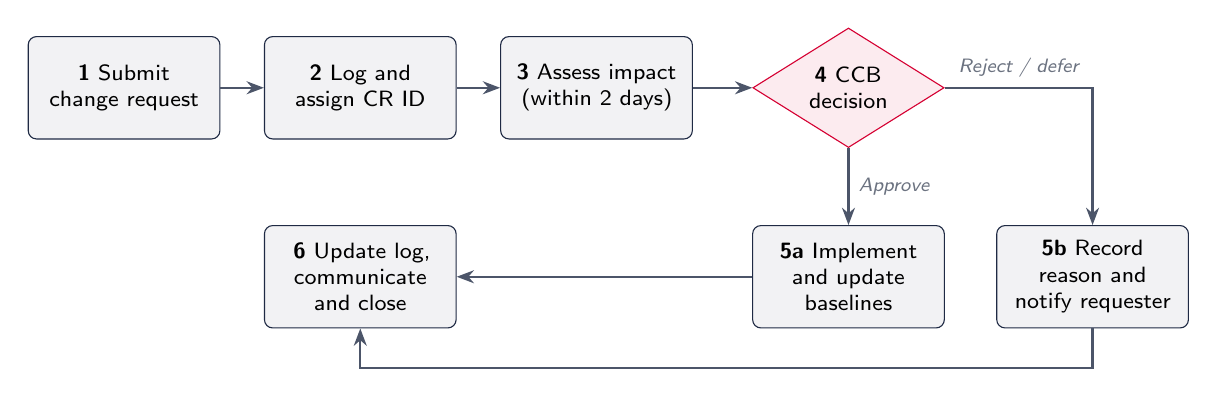
\begin{tikzpicture}[
    proc/.style={draw=brandprimary, fill=brandprimary!6, rounded corners=3pt, align=center,
                 font=\footnotesize\sffamily, text width=2.2cm, minimum height=1.3cm},
    decision/.style={diamond, draw=brandaccent, fill=brandaccent!8, align=center,
                     font=\footnotesize\sffamily, aspect=1.6, inner sep=1pt, text width=1.4cm},
    arrow/.style={-{Stealth[length=2.2mm]}, thick, brandprimary!80},
    lbl/.style={font=\scriptsize\sffamily\itshape, text=brandmuted}
]
  % Fixed coordinates keep the figure within the text width (about 14.7 cm)
  \node[proc] (submit) at (0,0) {\textbf{1} Submit change request};
  \node[proc] (log) at (3.0,0) {\textbf{2} Log and assign CR ID};
  \node[proc] (assess) at (6.0,0) {\textbf{3} Assess impact (within 2 days)};
  \node[decision] (decide) at (9.2,0) {\textbf{4} CCB decision};
  \node[proc] (implement) at (9.2,-2.4) {\textbf{5a} Implement and update baselines};
  \node[proc] (reject) at (12.3,-2.4) {\textbf{5b} Record reason and notify requester};
  \node[proc] (close) at (3.0,-2.4) {\textbf{6} Update log, communicate and close};

  \draw[arrow] (submit) -- (log);
  \draw[arrow] (log) -- (assess);
  \draw[arrow] (assess) -- (decide);
  \draw[arrow] (decide) -- node[lbl, right] {Approve} (implement);
  \draw[arrow] (decide.east) -| node[lbl, pos=0.25, above] {Reject / defer} (reject.north);
  \draw[arrow] (implement) -- (close);
  \draw[arrow] (reject.south) -- ++(0,-0.5) -| (close.south);
\end{tikzpicture}
\caption{Change control process}
\label{fig:change-control}
\end{figure}

\begin{enumerate}[nosep]
  \item \textbf{Submit.} The requester opens a GitHub issue labelled \texttt{change-request}, describing the change and the reason for it.
  \item \textbf{Log.} The Project Manager assigns a change request ID (CR-\textit{nnn}) and adds it to the change request log.
  \item \textbf{Assess impact.} The owners of the affected packages assess the impact on scope, schedule, effort, risks, quality and the requirements traceability (Table~\ref{tab:traceability}) within two days.
  \item \textbf{Decide.} The Change Control Board approves, rejects or defers the request at the next weekly meeting. Urgent requests can be decided by a vote in the messaging channel within 24 hours.
  \item \textbf{Implement or record.} Approved changes are implemented, and every affected baseline is updated: the requirements, WBS, schedule, risk register and this plan's version history. For rejected or deferred requests, the reason is recorded and the requester is notified.
  \item \textbf{Close.} The log is updated, and the decision is communicated to the team and, where relevant, to the tutor.
\end{enumerate}

\paragraph{Change freezes.} No scope changes are accepted after the code freeze (M12, 2 December), or within three days of any assessment deadline, except to fix critical defects. Each submitted version of the code is tagged in Git (e.g.\ \texttt{a2-submission}, \texttt{a3-submission}) so that it can always be recovered.

\subsection{Change Request Log}\label{sec:change-log}

Table~\ref{tab:change-log} shows the change request log. The three entries record major decisions made at team meetings while this plan was being prepared, before the baseline was set. They were assessed and agreed by the team in the same way, and are recorded in the minutes of Meetings~2 and~3. Future requests will be tracked through GitHub issues and added to this log.

{\renewcommand{\arraystretch}{1.2}\small
\begin{longtable}{@{}l l >{\raggedright\arraybackslash}p{0.33\textwidth} >{\raggedright\arraybackslash}p{0.27\textwidth} >{\raggedright\arraybackslash}p{0.11\textwidth}@{}}
  \caption{Change request log}\label{tab:change-log} \\
  \toprule
  \textbf{CR ID} & \textbf{Date} & \textbf{Change and Reason} & \textbf{Impact} & \textbf{Decision} \\
  \midrule
  \endfirsthead
  \multicolumn{5}{@{}l}{\small\itshape Table~\thetable{} continued} \\
  \toprule
  \textbf{CR ID} & \textbf{Date} & \textbf{Change and Reason} & \textbf{Impact} & \textbf{Decision} \\
  \midrule
  \endhead
  \bottomrule
  \endlastfoot
  CR-001 & 21 Sep & Adopt PRISMO \parencite{agrawal2018prismo} as the methodological basis and reproduce its method, rather than its exact results, to give the project a clear, evidence-based approach. & Requirements FR1--FR10 and WBS 2--4 restructured around PRISMO's three phases. & Approved (pre-baseline) \\
  CR-002 & 21 Sep & Add a moderator-centred decision-support focus and a user study (RQ2--RQ5) as the project's unique contribution. & New FR12, FR13, FR21--FR23 and NFR12; WBS 5.5, 6.3 and 6.4 added; about 36 hours added. & Approved (pre-baseline) \\
  CR-003 & 28 Sep & Align the plan with the unit's assessment brief and deadlines: interactive charts become Must, React and FastAPI are required, mobile responsiveness is added, and the dataset decision window shortens to one week. & FR17--FR19 and NFR7 updated; schedule rebuilt around three deadlines; effort re-estimated to 386 hours at 12 hours per member per week. & Approved (pre-baseline) \\
\end{longtable}
}

\clearpage
% =====================================================================
%  8. PROJECT CLOSURE PLAN
% =====================================================================
\section{Project Closure Plan}\label{sec:closure}

Project closure confirms that the project has delivered what it set out to deliver, hands its outputs over to the people who need them, and captures lessons for future projects \parencite{pmi2021pmbok}. Because \projectname{} produces deliverables at three assessment points, acceptance is checked at each submission, and the project is formally closed after Assignment~3.

\subsection{Acceptance Criteria}\label{sec:acceptance}

\paragraph{Acceptance process.} Each deliverable passes through two checks:

\begin{enumerate}[nosep]
  \item \textbf{Verification by the team.} At the pre-submission review two days before each deadline (Table~\ref{tab:reporting}), the team checks the deliverable against its acceptance criteria below and against the assessment brief. All four members sign off on the submission checklist.
  \item \textbf{Acceptance by the tutor.} The tutor, as assessor and client, formally accepts each deliverable through the unit's assessment process. Any feedback received before the next stage is reviewed at the following weekly meeting and, where needed, handled through change control.
\end{enumerate}

\paragraph{Project success criteria.} The project as a whole will be considered successful when the criteria in Table~\ref{tab:success-criteria} are met.

\begin{table}[htbp]
\centering
\caption{Project success criteria}
\label{tab:success-criteria}
\begin{tabularx}{\textwidth}{@{}>{\raggedright\arraybackslash}p{0.22\textwidth} >{\raggedright\arraybackslash}X >{\raggedright\arraybackslash}p{0.16\textwidth}@{}}
  \toprule
  \textbf{Criterion} & \textbf{Target} & \textbf{Linked To} \\
  \midrule
  Timeliness & All three assessments submitted on or before their deadlines (11 Oct, 2 Nov, 6 Dec) & M4, M9, M13 \\
  Requirements & 100\% of \textbf{Must} requirements implemented and verified, or formally changed through change control & Section~\ref{sec:requirements} \\
  Detection performance & Selected model achieves a macro-averaged F1-score of at least 0.85 and a spammer detection rate above 72.4\% on the held-out test set & O4, NFR1 \\
  Feature reduction & The PRISMO-selected subset (FS4) uses at most half of the original features, with a macro F1-score within 0.02 of the full-feature model & RQ1, FR6 \\
  Usability & System Usability Scale score of at least 68; a first-time user completes a single account check within one minute & NFR4 \\
  Research questions & RQ1--RQ5 are each answered with evidence in the assessment reports, with limitations stated where a contingency plan was used (e.g.\ R3) & Section~\ref{sec:rqs} \\
  Effort & Total actual effort stays within the team's capacity of about 456 hours & Section~\ref{sec:wbs-dictionary} \\
  Quality & No critical defects open at the code freeze (M12) & Table~\ref{tab:kpis} \\
  \bottomrule
\end{tabularx}
\end{table}

\paragraph{Deliverable acceptance criteria.} Table~\ref{tab:acceptance} defines the criteria each deliverable (Table~\ref{tab:deliverables}) must meet before it is submitted, and how each is verified.

{\renewcommand{\arraystretch}{1.2}\small
\begin{longtable}{@{}>{\raggedright\arraybackslash}p{0.15\textwidth} >{\raggedright\arraybackslash}p{0.48\textwidth} >{\raggedright\arraybackslash}p{0.27\textwidth}@{}}
  \caption{Deliverable acceptance criteria}\label{tab:acceptance} \\
  \toprule
  \textbf{Deliverable} & \textbf{Acceptance Criteria} & \textbf{Verification Method} \\
  \midrule
  \endfirsthead
  \multicolumn{3}{@{}l}{\small\itshape Table~\thetable{} continued} \\
  \toprule
  \textbf{Deliverable} & \textbf{Acceptance Criteria} & \textbf{Verification Method} \\
  \midrule
  \endhead
  \midrule
  \multicolumn{3}{@{}r}{\small\itshape Continued on next page} \\
  \endfoot
  \bottomrule
  \endlastfoot

  \multicolumn{3}{@{}l}{\cellcolor{brandprimary!8}\textbf{\sffamily Assignment 1 -- due Sun 11 Oct}} \\
  \textbf{D1} Project Management Plan &
  Contains every required section, including the front-end prototype and its alignment with usability principles; scope, schedule, effort and risks are consistent with each other; all sources are cited in Harvard style. &
  Checklist against the assessment brief; consistency check of requirement, WBS and milestone references \\

  \multicolumn{3}{@{}l}{\cellcolor{brandprimary!8}\textbf{\sffamily Assignment 2 -- due Mon 2 Nov}} \\
  \textbf{D2} Processed datasets &
  Provided as CSV/JSON; no missing or invalid values remain; training and test splits are stratified and documented; a data dictionary describes every feature; inclusion complies with the dataset's terms of use (R13). &
  Re-run the pre-processing pipeline from the raw data and confirm the outputs are identical \\
  \addlinespace
  \textbf{D3} Model source code and final models &
  Implements FR4--FR10: baseline, GA, PSO, SA and priority-based feature formation, and the four classifiers evaluated with 10-fold cross-validation; seeds and parameters are recorded (NFR9); the final model loads and returns predictions; NFR1 is met or the shortfall is documented. &
  Run the code in a clean environment by following the README; repeat one experiment with the same seed and compare results \\
  \addlinespace
  \textbf{D4} AI model report and README &
  Up to 3,000 words (PDF); answers RQ1 with a comparison against PRISMO's reported results; cites sources in Harvard style; the README lets someone outside the team run the code. &
  Word count; a member who did not write the README follows it from scratch \\

  \multicolumn{3}{@{}l}{\cellcolor{brandprimary!8}\textbf{\sffamily Assignment 3 -- due Sun 6 Dec}} \\
  \textbf{D5} Web application source code &
  All \textbf{Must} functional requirements are implemented, including the React front end, FastAPI back end with GET and POST endpoints, at least three interactive chart types, decision-support features and study mode; input is validated in both front end and back end; the layout is responsive (NFR7); response times meet NFR3; no critical defects; \texttt{node\_modules} is excluded from the ZIP file. &
  Every \textbf{Must} test case in the test plan (WBS 6.2) passes; requirements checklist signed off \\
  \addlinespace
  \textbf{D6} User study results &
  The study follows the approved protocol and any ethics requirements (NFR12); at least 8 participants take part, or the contingency plan for R3 or R4 is documented; RQ2--RQ5 are each answered with data; SUS scores are calculated correctly; all data is anonymous. &
  Analysis reviewed by a second member; raw data checked to confirm it contains no identifying information \\
  \addlinespace
  \textbf{D7} Web application report &
  Covers every section required by the brief: project title and group information on the cover, system architecture, front-end and back-end implementation with API documentation, AI model integration, conclusion and future work, Harvard-style bibliography and appendices; includes the user study findings. &
  Section-by-section checklist against the assessment brief \\
  \addlinespace
  \textbf{D8} Demonstration video &
  No longer than 7 minutes (MP4 or AVI); demonstrates every feature and interaction and the complete workflow from input to visualised results; shows responsiveness on desktop, tablet and mobile; explains key technical decisions and challenges. &
  Video script mapped to the feature list; final video timed and reviewed by all members \\

  \multicolumn{3}{@{}l}{\cellcolor{brandprimary!8}\textbf{\sffamily Closure -- Tue 8 Dec}} \\
  \textbf{D9} Lessons learned record &
  A retrospective is held with all members; lessons are recorded in the lessons learned register; the repository is tagged and archived. &
  Project Manager confirms the closure checklist (Section~\ref{sec:closure-activities}) \\
\end{longtable}
}

\subsection{Deliverable Handover}\label{sec:handover}

Table~\ref{tab:handover} lists what will be handed over, to whom and in what form.

\begin{table}[htbp]
\centering
\caption{Deliverable handover plan}
\label{tab:handover}
\begin{tabularx}{\textwidth}{@{}>{\raggedright\arraybackslash}p{0.27\textwidth} >{\raggedright\arraybackslash}p{0.14\textwidth} >{\raggedright\arraybackslash}X l l@{}}
  \toprule
  \textbf{Item} & \textbf{Recipient} & \textbf{Format and Location} & \textbf{Date} & \textbf{Owner} \\
  \midrule
  Assessment submissions (D1, D2--D4, D5--D8) & Tutor & PDF reports, ZIP files and MP4 video, submitted through the unit's learning management system & Each deadline & TKN \\
  \addlinespace
  Source code, final models and README & Tutor; team & GitHub repository tagged at each submission (\texttt{a2-submission}, \texttt{a3-submission}) & 6 Dec & HDN \\
  \addlinespace
  API documentation & Tutor; future developers & In the Assignment~3 report, and generated automatically by FastAPI as interactive OpenAPI documentation & 6 Dec & HDN \\
  \addlinespace
  Experiment records & Team; future researchers & Parameter and seed logs, results tables and feature subsets in the repository & 2 Nov & NKNT \\
  \addlinespace
  Project records & Team & Final plan, minutes, status reports, risk register and change log in the shared folder & 8 Dec & TKN \\
  \bottomrule
\end{tabularx}
\end{table}

\paragraph{Data handling at closure.} At closure, only anonymised user study results are kept. Any raw study data or consent records are retained or destroyed as required by Swinburne's guidance (NFR12). Local copies of datasets with restricted terms of use are deleted if their terms require it (R13). The repository is checked to ensure it contains no credentials or personal data before it is archived.

\subsection{Closure Activities and Lessons Learned}\label{sec:closure-activities}

\paragraph{Closure checklist.} The Project Manager is responsible for completing the following activities:

\begin{enumerate}[nosep]
  \item Confirm that every acceptance criterion in Table~\ref{tab:acceptance} has been met at the final pre-submission review (Fri 4 Dec).
  \item Submit Assignment~3 (Sun 6 Dec).
  \item Tag the final release in Git, then archive the repository and project documents.
  \item Complete the data handling steps above.
  \item Close the risk register and change log, recording the final status of every risk and change request.
  \item Produce a final effort report comparing actual and estimated hours for each work package.
  \item Hold the final retrospective (Tue 8 Dec) and record lessons learned.
  \item Formally close the project and confirm with all members that no outstanding actions remain.
\end{enumerate}

\paragraph{Lessons learned.} Lessons are captured throughout the project rather than only at the end, so that they can be applied while the project is still running. A short \textbf{stage retrospective} is held at the first weekly meeting after Assignment~1 and Assignment~2, and lessons from Stage~2 (such as the accuracy of effort estimates and how the dataset risk played out) are applied to the plan for Stage~3. The \textbf{final retrospective} on 8 December reviews the whole project using three questions: \emph{what went well}, \emph{what did not go well}, and \emph{what should be done differently next time}. It draws on objective records, including planned versus actual milestones, the weekly SPI and EPI history, the risks that occurred compared with those predicted, and the change request log.

Each lesson is recorded in the lessons learned register (Table~\ref{tab:lessons}) with a concrete recommendation, so that it can be reused by team members in future projects.

\begin{table}[htbp]
\centering
\caption{Lessons learned register (structure)}
\label{tab:lessons}
\begin{tabularx}{\textwidth}{@{}l l >{\raggedright\arraybackslash}p{0.17\textwidth} >{\raggedright\arraybackslash}X >{\raggedright\arraybackslash}X@{}}
  \toprule
  \textbf{ID} & \textbf{Stage} & \textbf{Category} & \textbf{What Happened and Its Impact} & \textbf{Recommendation} \\
  \midrule
  LL-\textit{nn} & 1--4 & Planning, Technical, Team or Stakeholder & Description of the event or observation and its effect on the project & Specific action to repeat or avoid in future projects \\
  \midrule
  \multicolumn{5}{@{}l}{\footnotesize\itshape Completed at each stage retrospective and at the final retrospective.} \\
  \bottomrule
\end{tabularx}
\end{table}

\clearpage
% =====================================================================
%  9. PROJECT DESIGN
% =====================================================================
\section{Project Design}\label{sec:design}

This section presents the planned system architecture, the front-end prototype of \projectname{}, and how the design applies recognised usability principles. The design follows the project's research focus (Section~\ref{sec:rqs}): the interface is meant not only to display predictions, but to help moderators review accounts accurately, efficiently and with an appropriate level of trust in the model.


\subsection{System Overview}\label{sec:system-overview}

\projectname{} integrates a data pipeline, a machine learning model layer, an API and a front end into a single architecture (Figure~\ref{fig:architecture}).

\begin{figure}[htbp]
\centering
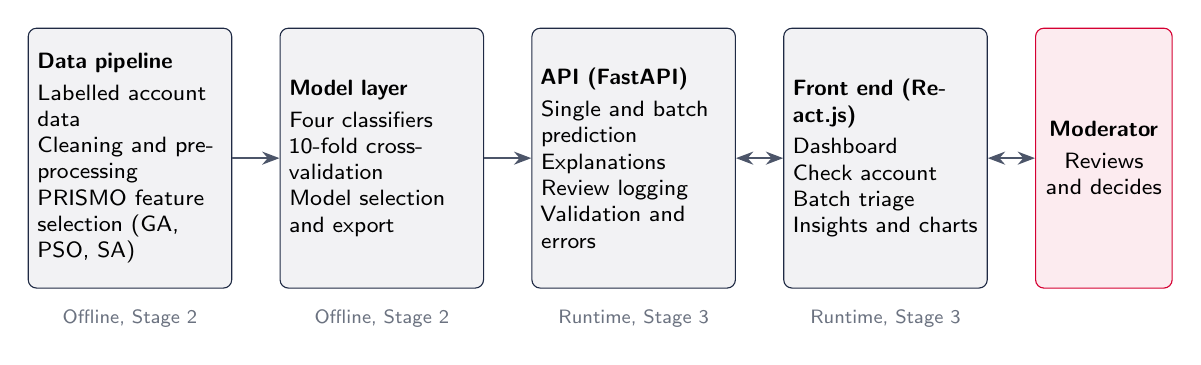
\begin{tikzpicture}[
    node distance=0.6cm,
    tierbox/.style={draw=brandprimary, fill=brandprimary!6, rounded corners=3pt, align=left,
                  font=\footnotesize\sffamily, text width=2.35cm, minimum height=3.3cm},
    actor/.style={draw=brandaccent, fill=brandaccent!8, rounded corners=3pt, align=center,
                  font=\footnotesize\sffamily, text width=1.5cm, minimum height=3.3cm},
    arrow/.style={-{Stealth[length=2.2mm]}, thick, brandprimary!80},
    both/.style={{Stealth[length=2.2mm]}-{Stealth[length=2.2mm]}, thick, brandprimary!80},
    stage/.style={font=\scriptsize\sffamily, text=brandmuted}
]
  \node[tierbox] (data) {\textbf{Data pipeline}\\[2pt]Labelled account data\\Cleaning and pre-processing\\PRISMO feature selection (GA, PSO, SA)};
  \node[tierbox, right=of data] (model) {\textbf{Model layer}\\[2pt]Four classifiers\\10-fold cross-validation\\Model selection and export};
  \node[tierbox, right=of model] (api) {\textbf{API (FastAPI)}\\[2pt]Single and batch prediction\\Explanations\\Review logging\\Validation and errors};
  \node[tierbox, right=of api] (fe) {\textbf{Front end (React.js)}\\[2pt]Dashboard\\Check account\\Batch triage\\Insights and charts};
  \node[actor, right=of fe] (user) {\textbf{Moderator}\\[2pt]Reviews and decides};

  \draw[arrow] (data) -- (model);
  \draw[arrow] (model) -- (api);
  \draw[both] (api) -- (fe);
  \draw[both] (fe) -- (user);

  \node[stage, below=0.15cm of data] {Offline, Stage 2};
  \node[stage, below=0.15cm of model] {Offline, Stage 2};
  \node[stage, below=0.15cm of api] {Runtime, Stage 3};
  \node[stage, below=0.15cm of fe] {Runtime, Stage 3};
\end{tikzpicture}
\caption{System architecture of \projectname{}}
\label{fig:architecture}
\end{figure}

\begin{itemize}[nosep]
  \item \textbf{Data pipeline.} Prepares the labelled account data, then applies feature preparation and PRISMO's two-layer feature selection (Section~\ref{sec:prismo}).
  \item \textbf{Model layer.} Trains and compares Random Forest, Na\"ive Bayes, a rule-based learner and a decision tree, then exports the best-performing model together with its pre-processing and feature-selection steps.
  \item \textbf{API (FastAPI).} Loads the exported model and provides endpoints for single-account checks, batch triage, explanations and moderator reviews, with input validation and error handling. Because the same pre-processing is used for training and prediction, results in the application are consistent with the evaluated model (R10).
  \item \textbf{Front end (React.js).} Provides moderators with a dashboard, input forms, batch triage tools and interactive visualisations (built with a library such as Plotly.js), communicating with the API through JSON over HTTP.
\end{itemize}

Table~\ref{tab:api} lists the planned API endpoints. They use both the GET and POST methods required by the unit and correspond directly to actions in the prototype.

\begin{table}[htbp]
\centering
\caption{Planned API endpoints}
\label{tab:api}
\begin{tabularx}{\textwidth}{@{}l >{\raggedright\arraybackslash}p{0.25\textwidth} >{\raggedright\arraybackslash}X l@{}}
  \toprule
  \textbf{Method} & \textbf{Endpoint} & \textbf{Purpose} & \textbf{Req.} \\
  \midrule
  GET  & \texttt{/api/features} & Names, units and valid ranges of the selected features; drives manual input and its validation & FR15, FR18 \\
  GET  & \texttt{/api/samples} & Sample accounts for the \emph{Sample Account} selector & FR15 \\
  POST & \texttt{/api/predict} & Score one account; returns the label, spam score, review flag and explanation & FR11--FR13 \\
  POST & \texttt{/api/batches} & Validate an uploaded batch and score every account & FR16, FR18 \\
  POST & \texttt{/api/reviews} & Save a moderator's decision and notes, keeping the original prediction unchanged & FR21, FR23 \\
  GET  & \texttt{/api/batches/\{id\}/export} & Export predictions, decisions and review notes as CSV & FR16 \\
  GET  & \texttt{/api/metrics} & Model evaluation and feature selection results for the insights page & FR14, FR19 \\
  \bottomrule
\end{tabularx}
\end{table}

\subsection{Front-end Prototype}\label{sec:prototype}

The front-end prototype was designed in Figma by \memberFour{} as a clickable prototype with interactions. It uses illustrative data throughout, which is marked by a \emph{Demo mode} badge and a footer reminding users that data is illustrative and human review is required. Every screen shares the same layout: a navy sidebar with four workspace areas (Dashboard, Check account, Batch triage and Insights), a breadcrumb, and a consistent colour code of red for \emph{likely spam}, amber for \emph{needs review} and teal for \emph{likely genuine}.
\href{https://www.figma.com/design/4Z7n5mLQY9oHJUmVBQmA1i/SpamSentinel?node-id=1-2&t=1zb9kp3R3MiX9RbX-1}{(Click to view SpamSentinel Figma prototype)}

The prototype follows a moderator's workflow from start to finish. The moderator signs in to the workspace and lands on the dashboard. From there, they check a single account or load a batch, inspect the explanation for a flagged account, record a review decision, and export the results. Figures~\ref{fig:proto-login}--\ref{fig:proto-mobile} show the main desktop screens and the mobile view.

\paragraph{Sign-in (Figure~\ref{fig:proto-login}).} The entry screen introduces \projectname{} as a \emph{moderator workspace}, with an example account card that previews what the tool does: a spam score and the signals behind it. The prototype also shows a \emph{Sign Up} button, but self-registration will not be implemented. Account registration and stored user accounts remain out of scope (Table~\ref{tab:in-out-scope}).

\begin{figure}[htbp]
\centering
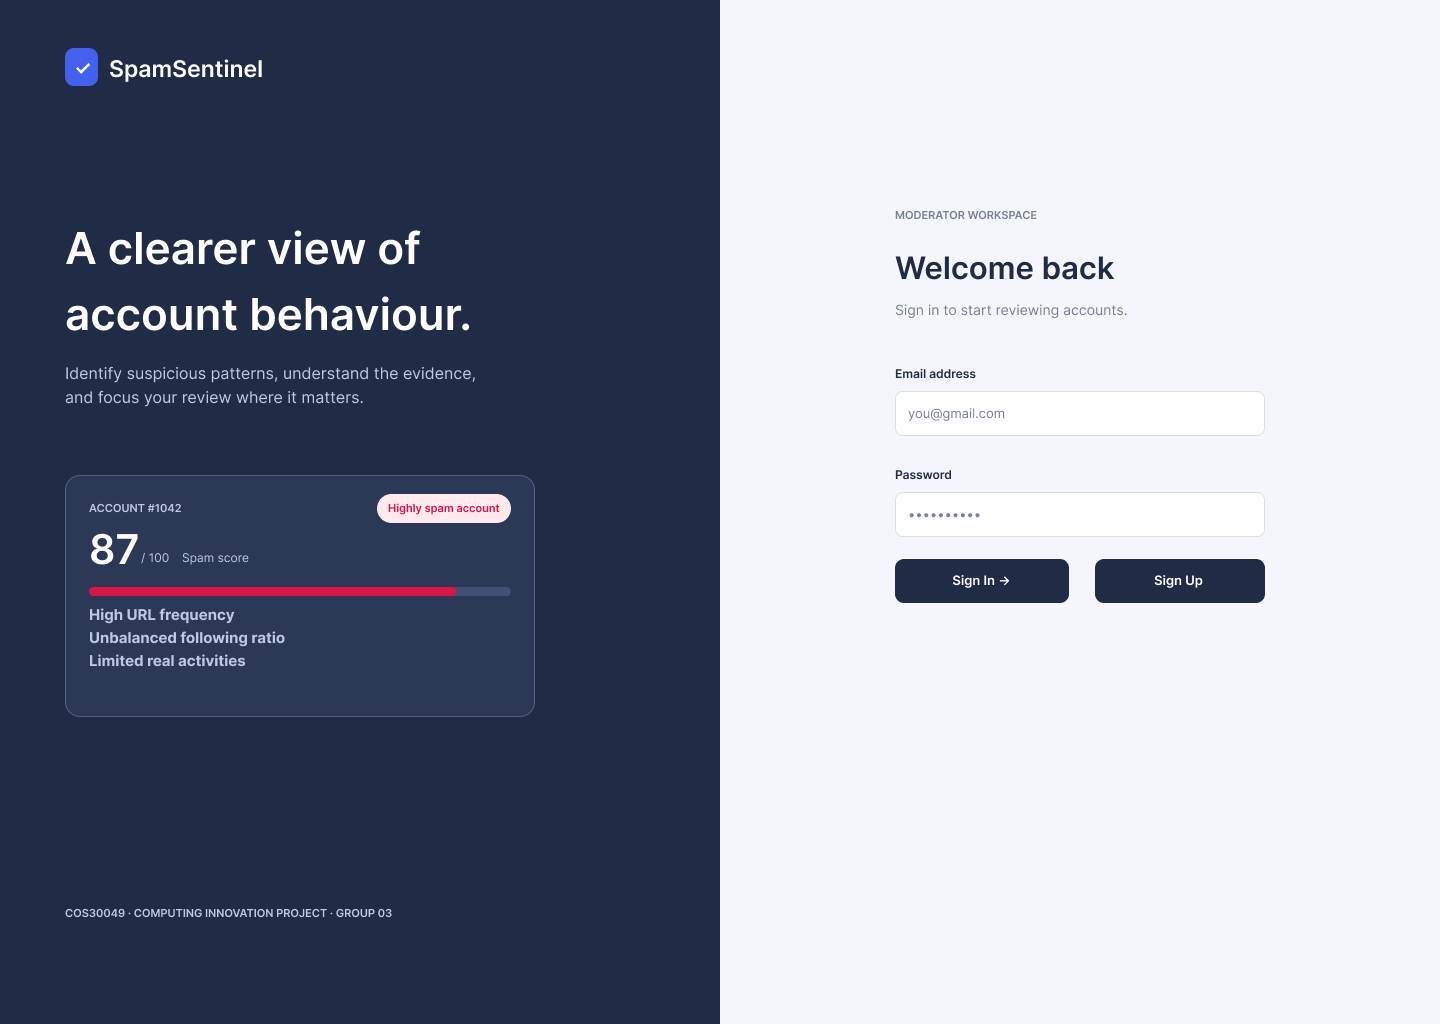
\includegraphics[width=0.92\textwidth]{proto-login}
\caption{Prototype: sign-in screen for the moderator workspace}
\label{fig:proto-login}
\end{figure}

\paragraph{Dashboard (Figure~\ref{fig:proto-dashboard}).} The \emph{Account review overview} summarises the current batch in four cards (accounts analysed, likely spam, needs review and likely genuine). It shows the distribution of spam scores in a histogram, tracks review progress, and lists a priority review queue. Two shortcuts start the main tasks: \emph{Check an Account} and \emph{Upload Account Batch}. The note \enquote{Model predictions stay separate from your decisions} reinforces that the moderator, not the model, makes the final call (FR16, FR19).

\begin{figure}[htbp]
\centering
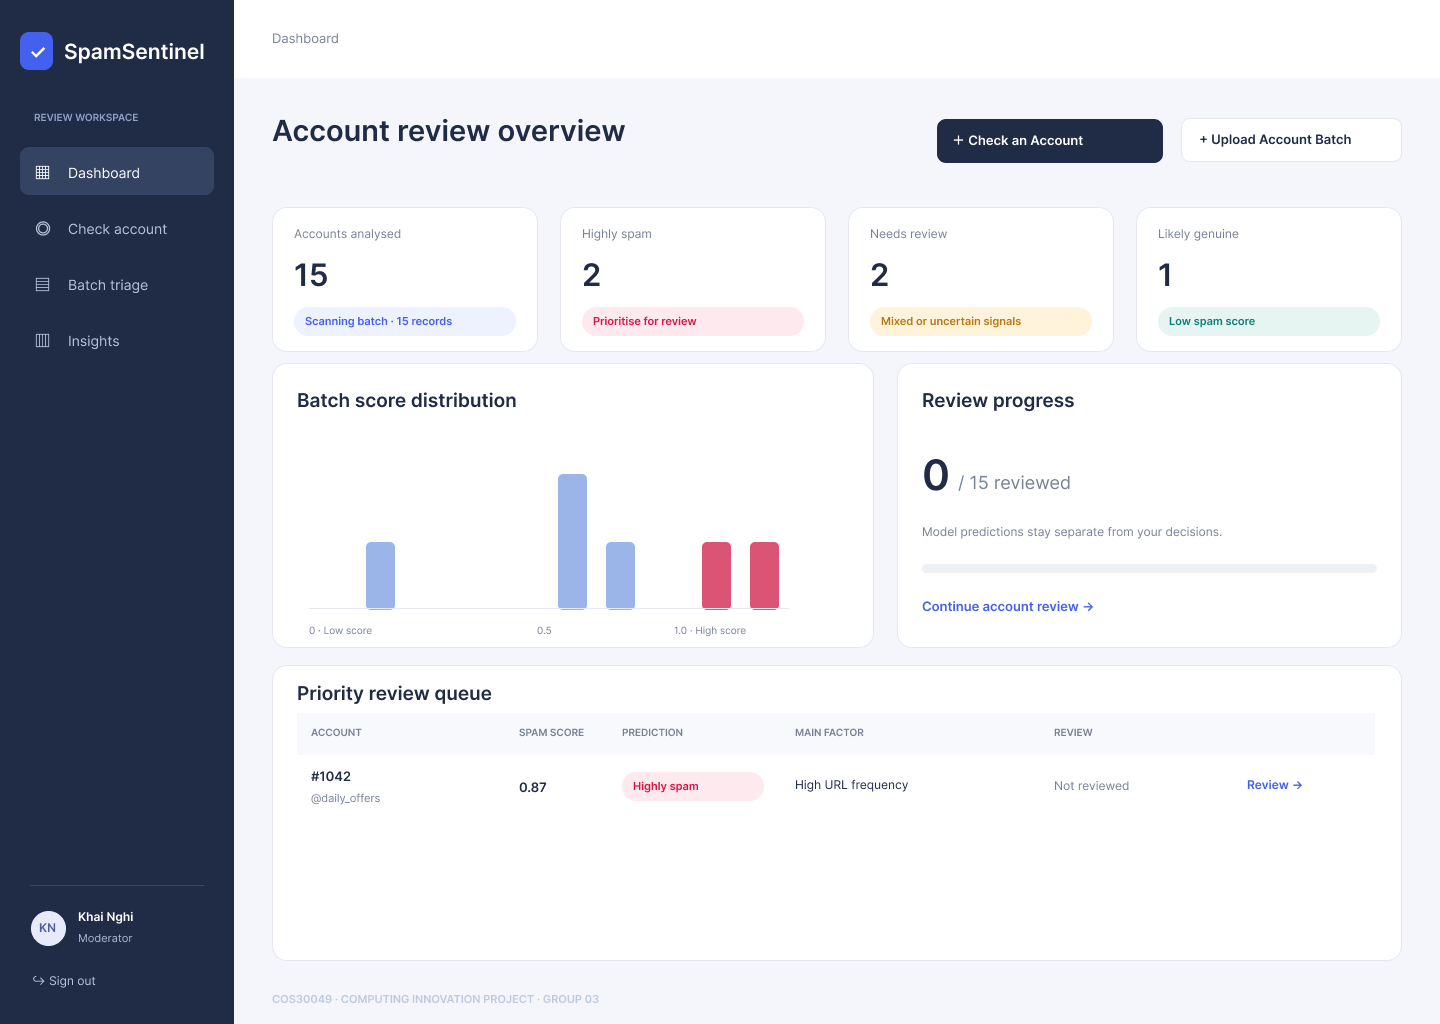
\includegraphics[width=0.92\textwidth]{proto-dashboard}
\caption{Prototype: dashboard with summary cards, score distribution, review progress and priority queue}
\label{fig:proto-dashboard}
\end{figure}

\paragraph{Single account check (Figure~\ref{fig:proto-check}).} Moderators can choose a sample account or switch to the \emph{Input Account Information} tab to enter feature values manually (FR15). A feature preview shows the key values before analysis. The result panel then presents the prediction label, the spam score with a score bar, and the three key signals to review, in plain language (FR12). From the result, the moderator can open the full explanation or record a review. Before an account is analysed, an empty state explains what to do next (\enquote{Ready to analyse}).

\begin{figure}[htbp]
\centering
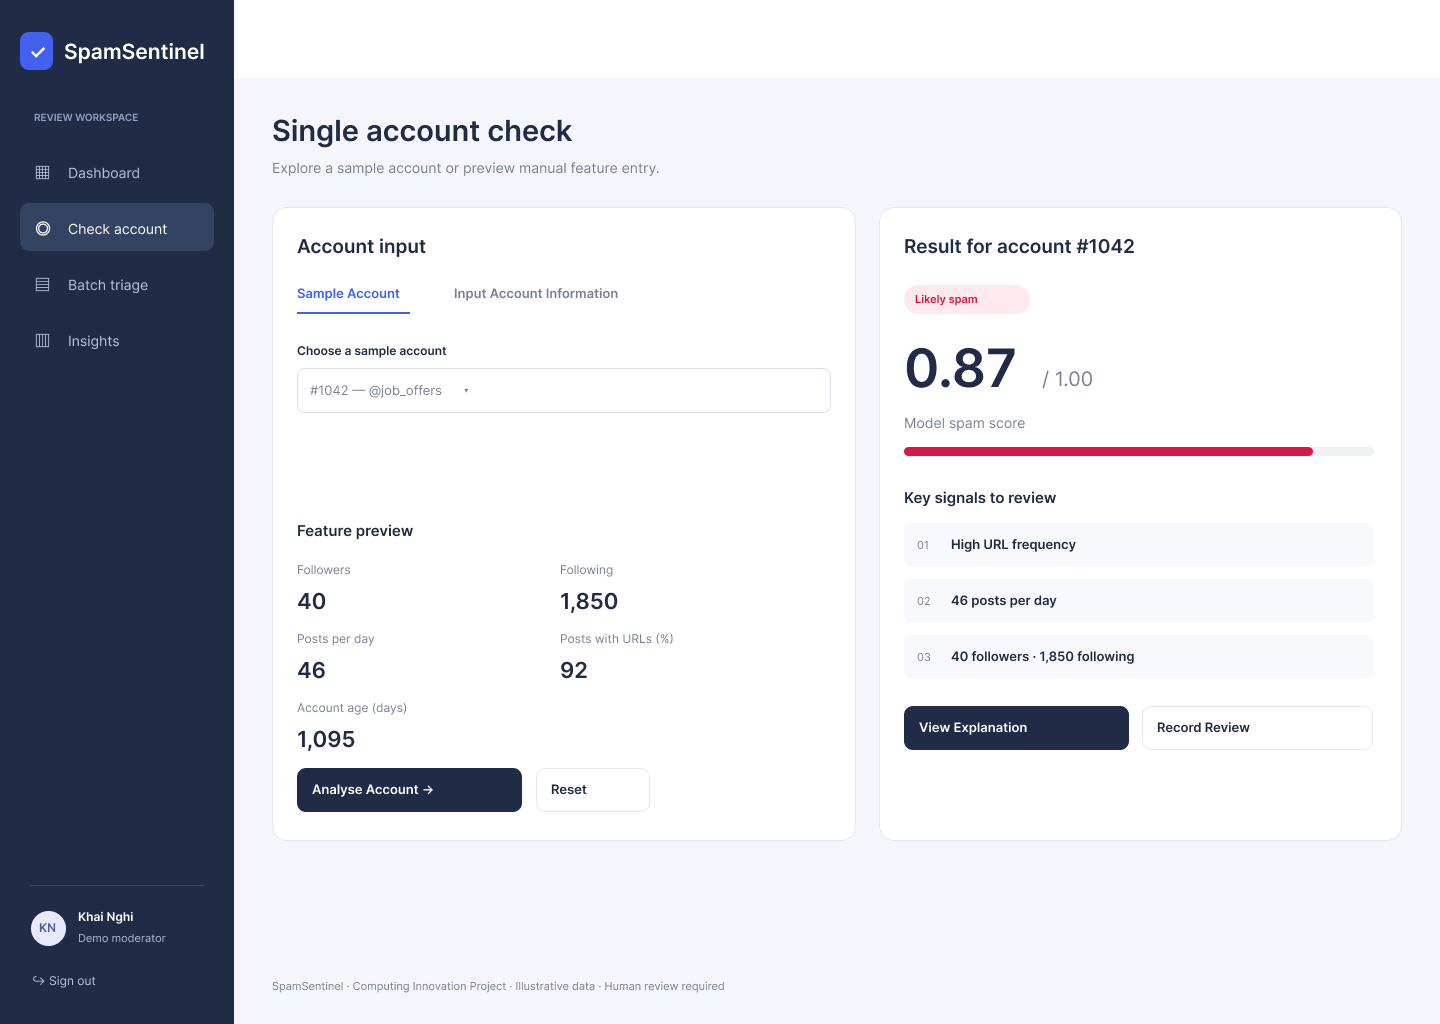
\includegraphics[width=0.92\textwidth]{proto-check}
\caption{Prototype: single account check with feature preview, spam score and key signals}
\label{fig:proto-check}
\end{figure}

\paragraph{Batch triage (Figure~\ref{fig:proto-batch}).} A batch is processed in three steps: load the accounts, validate the features (required columns and numeric values), and review the predictions. The account review queue is sorted by spam score and shows each account's prediction, main factor and review status. It can be searched and filtered by prediction. Moderators can start a new batch, clear filters, and export the predictions together with their decisions and review notes (FR16, FR18).

\begin{figure}[htbp]
\centering
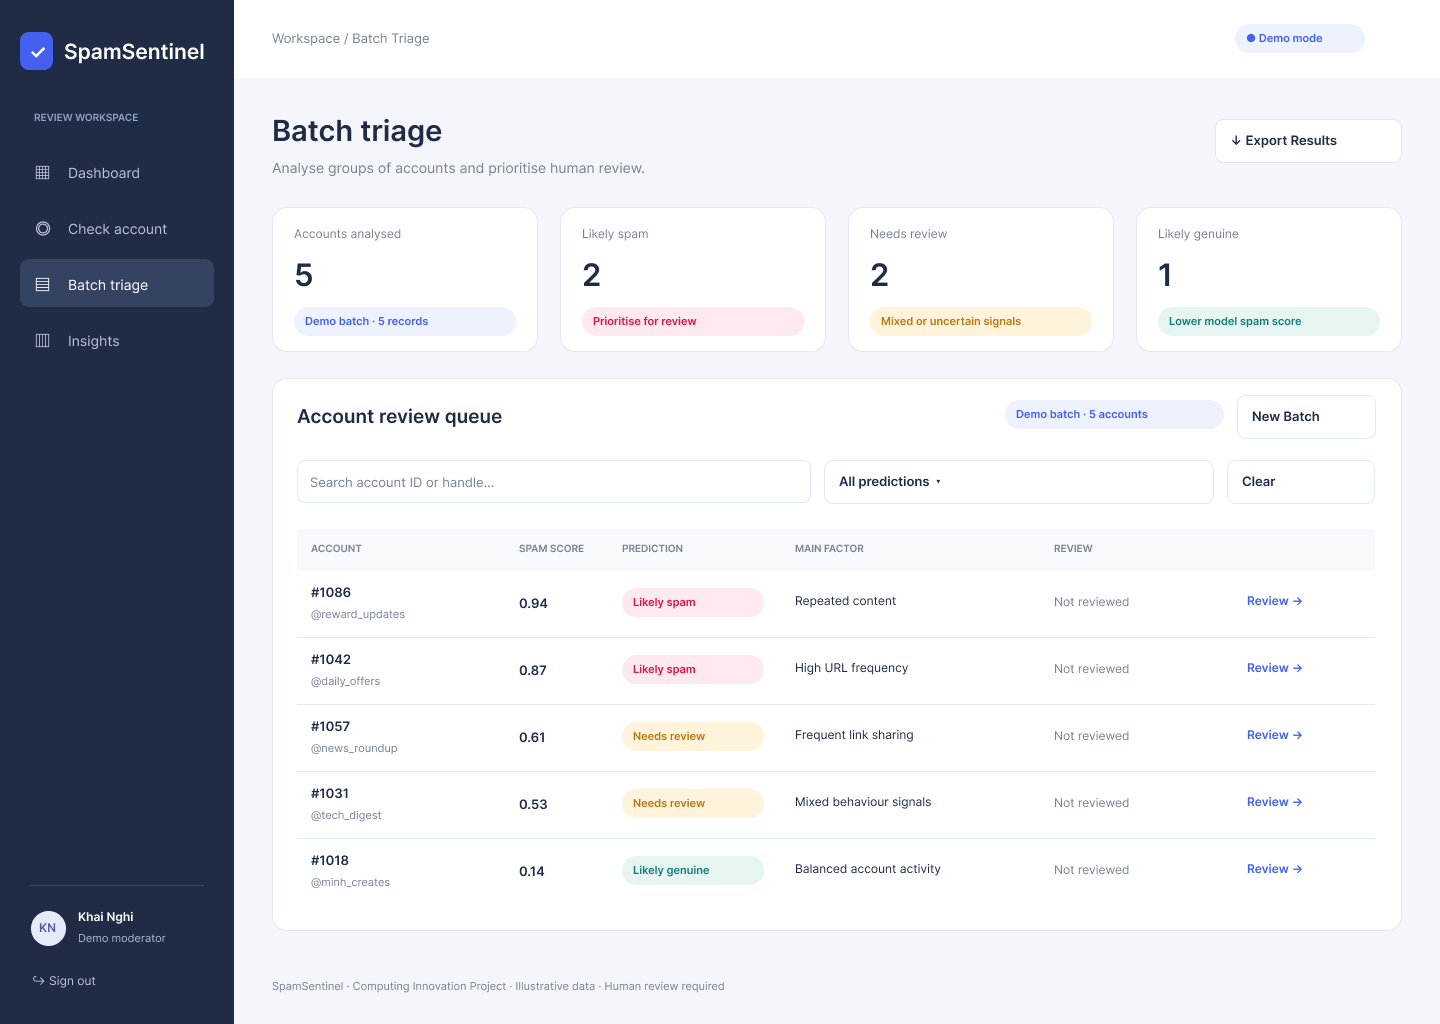
\includegraphics[width=0.92\textwidth]{proto-batch}
\caption{Prototype: batch triage queue sorted by spam score, with search, filtering and export}
\label{fig:proto-batch}
\end{figure}

\paragraph{Human review panel (Figure~\ref{fig:proto-review}).} Selecting \emph{Review} opens a side panel with the account's prediction, spam score and main factor, a link to the full explanation, a decision selector and a field for review notes (FR21). After the review is saved, the queue confirms \enquote{Review recorded for account \#1042. Original prediction preserved}, and the row's status changes to \emph{Reviewed}. Keeping the model's prediction separate from the moderator's decision also makes it possible to measure how often users override the model, which is central to RQ4 (FR23).

\begin{figure}[htbp]
\centering
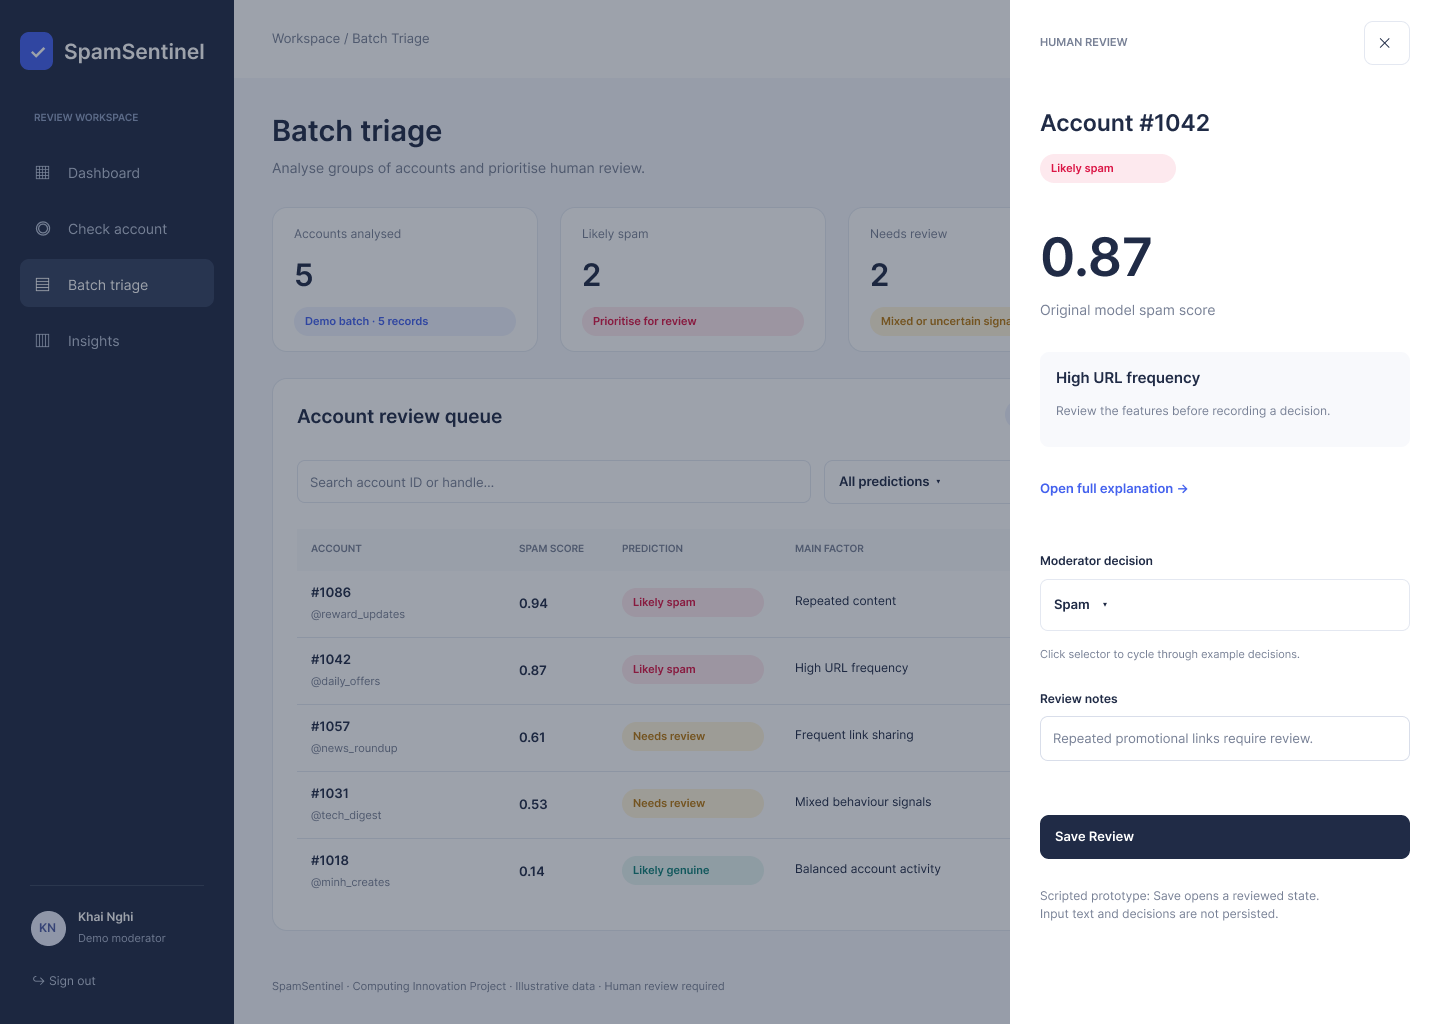
\includegraphics[width=0.92\textwidth]{proto-review}
\caption{Prototype: human review panel for recording a moderator decision and notes}
\label{fig:proto-review}
\end{figure}

\paragraph{Account explanation (Figure~\ref{fig:proto-explanation}).} The \emph{Explanation \& insights} page shows why an account received its score. A contribution chart shows how much each feature increased (red) or decreased (teal) the score, with details available on hover (FR11, FR19). Alongside it, \emph{feature evidence} cards explain each factor in plain language and compare it with a genuine-account reference, for example \enquote{92\% of posts contain URLs \ldots\ genuine reference: under 20\%} (FR12). A note confirms that raw posts, comments and private messages are not included, reflecting the project's privacy requirement (NFR10).

\begin{figure}[htbp]
\centering
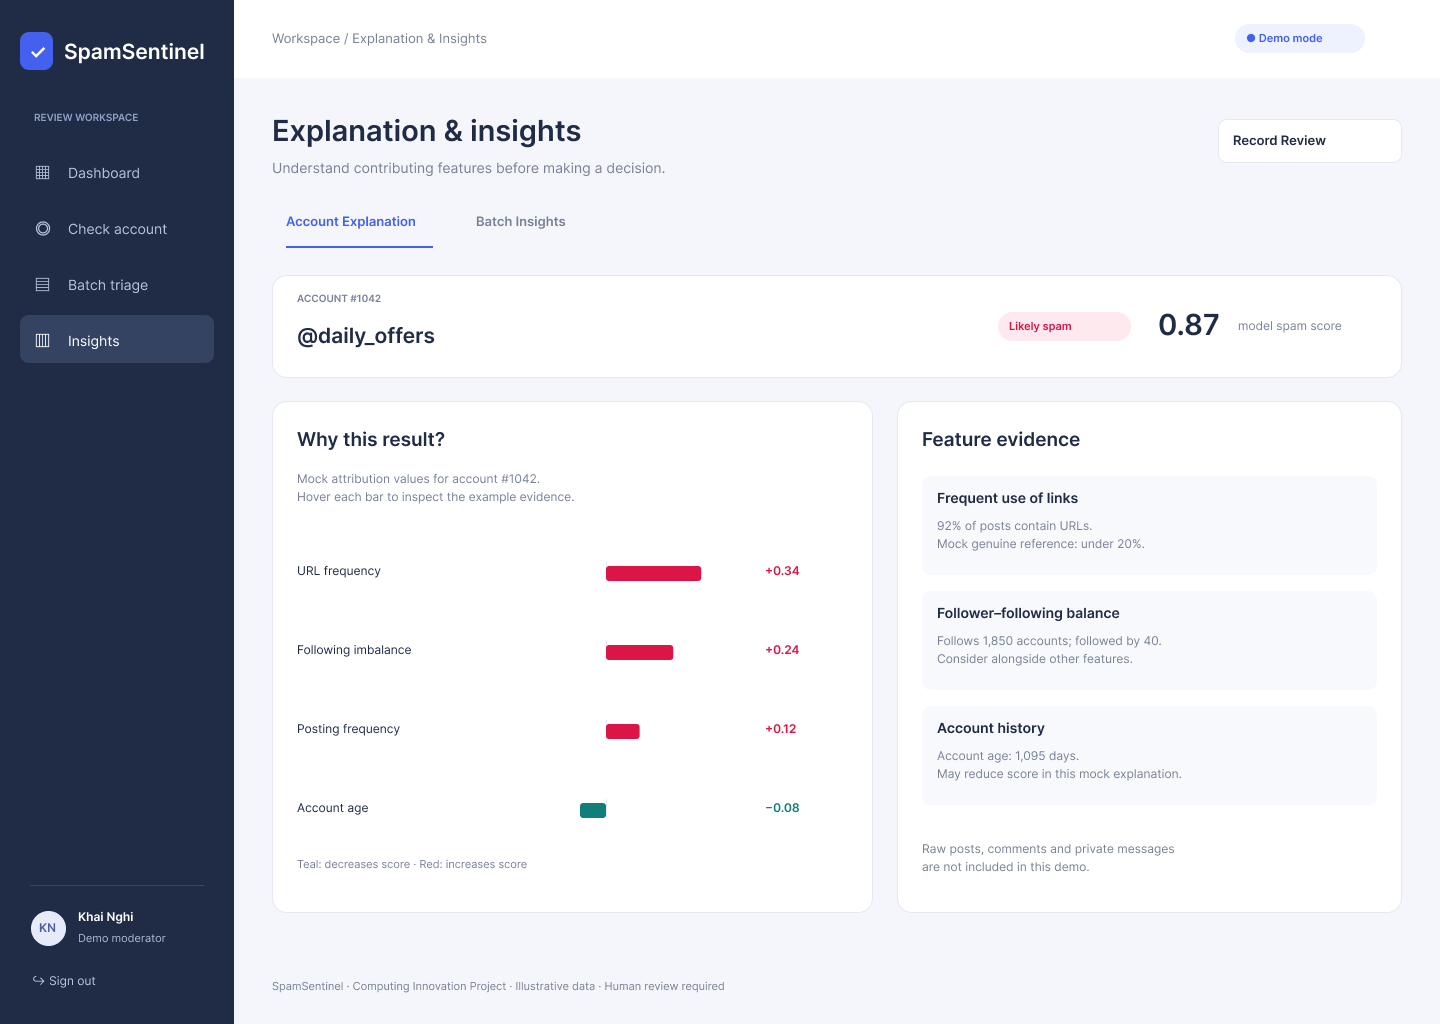
\includegraphics[width=0.92\textwidth]{proto-explanation}
\caption{Prototype: account explanation with feature contribution chart and plain-language feature evidence}
\label{fig:proto-explanation}
\end{figure}

\paragraph{Batch insights (Figure~\ref{fig:proto-insights}).} The \emph{Batch Insights} tab shows the score distribution of the current batch as an interactive histogram. The \emph{Model evaluation} panel is deliberately left as a placeholder (\enquote{Awaiting experimental results}): no performance values are claimed until the experiments in Stage~2 are complete. After Assignment~2, this panel will compare precision, recall and F1-score across classifiers and feature sets (FR9, FR14).

\begin{figure}[htbp]
\centering
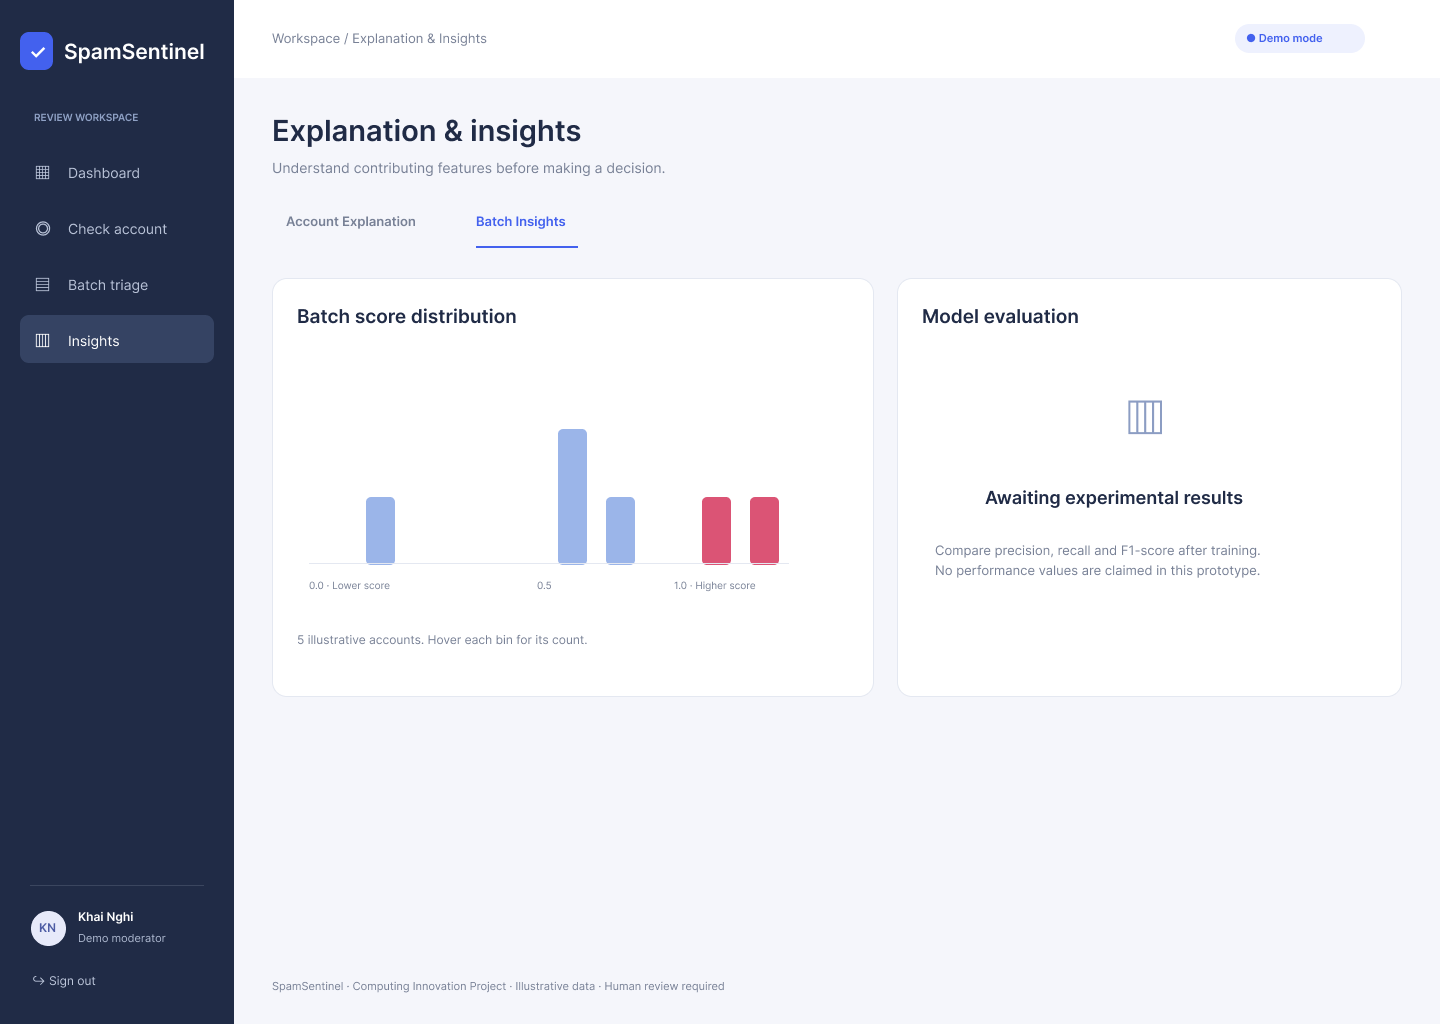
\includegraphics[width=0.92\textwidth]{proto-insights}
\caption{Prototype: batch insights with score distribution and the model evaluation panel awaiting results}
\label{fig:proto-insights}
\end{figure}

\paragraph{Mobile view (Figure~\ref{fig:proto-mobile}).} The mobile prototype adapts the same workflow to a phone screen, using the same colours, badges and wording as the desktop design (NFR7):

\begin{itemize}[nosep]
  \item \textbf{Navigation.} The sidebar is replaced by a bottom tab bar (Dashboard, Check, Batch and Insights), which keeps the four workspace areas within thumb reach.
  \item \textbf{Layout.} Cards stack in a single column and the summary cards form a two-by-two grid.
  \item \textbf{Touch targets.} Primary actions become full-width buttons.
  \item \textbf{Account result.} The score bar marks the uncertainty \emph{review zone} directly (FR13), so users can see how close an account is to needing human review.
  \item \textbf{Review sheet.} Recording a review opens a bottom sheet over the queue, with a three-way decision control (Spam, Genuine or Escalate), review notes, and a reminder that the original model prediction is kept alongside the moderator's decision (FR21).
\end{itemize}

\begin{figure}[htbp]
\centering
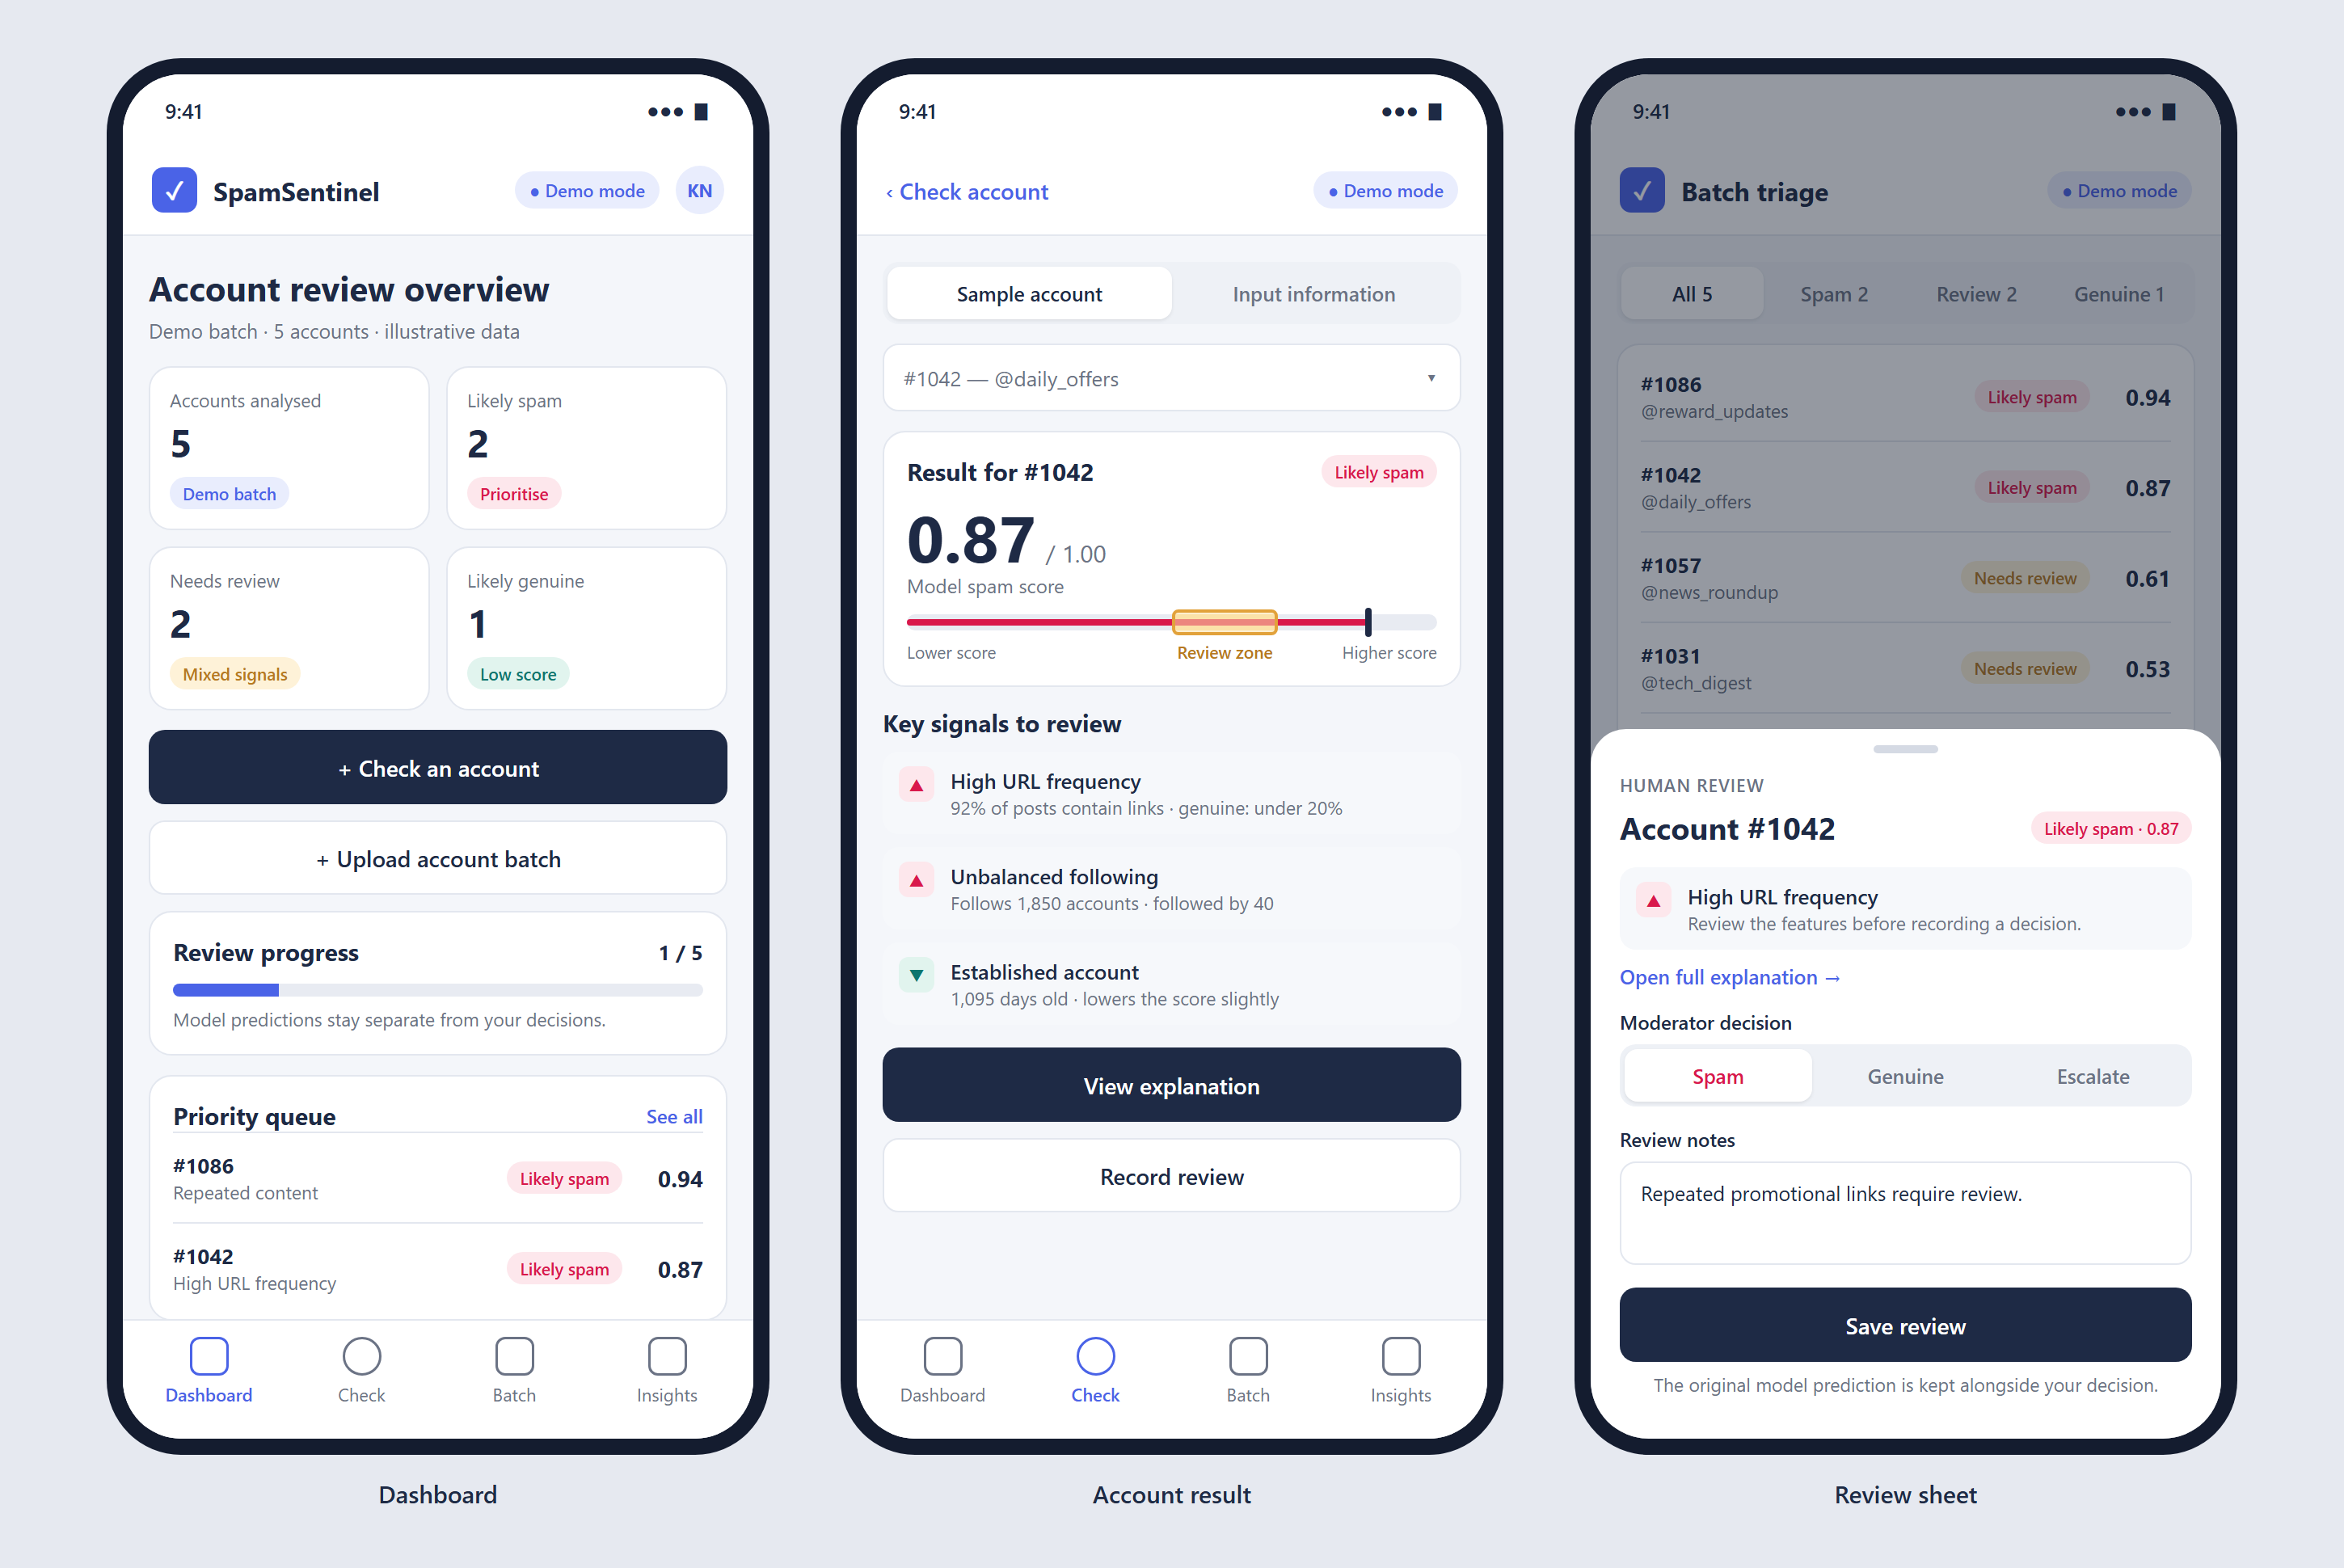
\includegraphics[width=\textwidth]{proto-mobile}
\caption{Prototype: mobile view of the dashboard, account result and human review sheet}
\label{fig:proto-mobile}
\end{figure}

\paragraph{Planned refinements.} The prototype will be refined before milestone M6 (Section~\ref{sec:milestones}) based on a heuristic review by the team:

\begin{itemize}[nosep]
  \item design the manual input form for the selected features, with units, valid ranges and field-level error messages (FR15, FR18);
  \item bring the review zone shown on the mobile score bar into the desktop design, so that users can see why an account needs review (FR13);
  \item add the model evaluation chart once results are available, giving at least three interactive chart types (FR19);
  \item design tablet layouts and mobile versions of the explanation and insights screens (NFR7); and
  \item use the same label wording (e.g.\ \emph{Likely spam}) on every screen.
\end{itemize}

\subsection{Alignment with Usability Principles}\label{sec:usability}

The design follows Nielsen's ten usability heuristics \parencite{nielsen1994heuristics}. It offers clear system feedback, plain-language explanations and consistent layouts. Moderators keep control through review and override options, and errors are prevented through validation and uncertainty warnings. Table~\ref{tab:heuristics} shows how each heuristic is applied in the prototype.

{\renewcommand{\arraystretch}{1.2}\small
\begin{longtable}{@{}>{\raggedright\arraybackslash}p{0.22\textwidth} >{\raggedright\arraybackslash}p{0.58\textwidth} >{\raggedright\arraybackslash}p{0.12\textwidth}@{}}
  \caption{Application of Nielsen's usability heuristics in the prototype}\label{tab:heuristics} \\
  \toprule
  \textbf{Heuristic} & \textbf{How the Design Applies It} & \textbf{Figures} \\
  \midrule
  \endfirsthead
  \multicolumn{3}{@{}l}{\small\itshape Table~\thetable{} continued} \\
  \toprule
  \textbf{Heuristic} & \textbf{How the Design Applies It} & \textbf{Figures} \\
  \midrule
  \endhead
  \bottomrule
  \endlastfoot
  1. Visibility of system status & A step indicator shows progress through batch processing; review progress (\enquote{0 / 15 reviewed}) and each account's review status are always visible; saving a review produces an immediate confirmation; filtered views state how many accounts are shown. & \ref{fig:proto-dashboard}, \ref{fig:proto-batch}, \ref{fig:proto-review} \\
  2. Match between system and the real world & Factors are described in plain language (\enquote{High URL frequency}, \enquote{Follows 1,850 accounts; followed by 40}) and compared with genuine-account references; categories and actions use moderators' own vocabulary: likely spam, needs review, review notes. & \ref{fig:proto-check}, \ref{fig:proto-explanation} \\
  3. User control and freedom & Moderators can reset inputs, clear filters, start a new batch, close panels and dialogs, and change or override the model's prediction, while the original prediction is preserved. & \ref{fig:proto-batch}, \ref{fig:proto-review} \\
  4. Consistency and standards & The sidebar, breadcrumb, footer, card style and colour-coded badges are identical on every screen, so the same prediction looks the same wherever it appears. & All \\
  5. Error prevention & Sample accounts avoid manual-entry mistakes; batches are validated for required columns and numeric values before analysis; a separate \emph{needs review} category avoids forcing uncertain cases into a label. & \ref{fig:proto-check}, \ref{fig:proto-batch} \\
  6. Recognition rather than recall & Each queue row shows its main factor; key signals appear next to the score; evidence cards sit beside the chart; decisions are chosen from a selector rather than typed. & \ref{fig:proto-check}, \ref{fig:proto-review}, \ref{fig:proto-explanation} \\
  7. Flexibility and efficiency of use & Dashboard shortcuts start the two main tasks; the queue is sorted by spam score so the riskiest accounts come first; search, filters and export speed up work on large batches. & \ref{fig:proto-dashboard}, \ref{fig:proto-batch} \\
  8. Aesthetic and minimalist design & Only the three key signals are shown by default, with full detail one click away; each panel has a single primary action; no model performance figures are shown until real results exist. & \ref{fig:proto-check}, \ref{fig:proto-insights} \\
  9. Help users recognise, diagnose and recover from errors & Batch validation reports missing columns or non-numeric values before analysis; an empty filtered view explains how to restore all results; manual input will show field-level messages explaining how to correct each value. & \ref{fig:proto-batch} \\
  10. Help and documentation & Page subtitles explain each screen's purpose; chart legends explain colours (\enquote{Teal: decreases score · Red: increases score}); hover details and inline guidance (\enquote{Review the features before recording a decision}) support users at the point of need. & \ref{fig:proto-review}, \ref{fig:proto-explanation} \\
\end{longtable}
}

\paragraph{Designing for appropriate trust.} Because \projectname{} supports human decisions, the design aims to make users trust the model only as much as it deserves. Explanations let moderators check each prediction against the evidence. The \emph{needs review} category signals when the model is unsure. Messages such as \enquote{Human review required} and \enquote{Original prediction preserved} make clear that the model advises rather than decides. Whether these choices improve decision accuracy and reduce over-reliance is tested directly by RQ3 and RQ4.

\paragraph{Accessibility and responsiveness.} Prediction categories are always shown as text labels, not by colour alone, and colours will be checked against WCAG 2.1 Level AA contrast guidelines \parencite{w3c2018wcag21}. The React implementation will use a responsive layout for desktop, tablet and mobile screens, following the mobile prototype in Figure~\ref{fig:proto-mobile} (NFR6, NFR7).

\paragraph{Evaluation of the design.} The team will carry out a heuristic evaluation of the refined prototype against Table~\ref{tab:heuristics} before M6. The finished application will then be evaluated with users in the study, using task time, decision accuracy and the System Usability Scale \parencite{brooke1996sus}, against the target of a score of at least 68 (NFR4).

\clearpage
% =====================================================================
%  10. CONCLUSION
% =====================================================================
\section{Conclusion}\label{sec:conclusion}

Spam accounts remain a persistent cybersecurity problem on social media. They spread scams, malicious links and misleading content, and they increasingly imitate genuine users to avoid detection. This plan sets out how \teamname{} will deliver \projectname{}, an explainable, moderator-centred tool for detecting spam accounts, within the \unitcode{} timeframe.

The project combines a proven method with a distinct contribution. Technically, it reproduces the PRISMO approach \parencite{agrawal2018prismo}: two-layer feature selection using GA, PSO and SA, followed by a comparison of four classifiers on labelled data from real accounts. It reports honestly where its results agree with, or differ from, the original paper. Beyond reproduction, the project treats spam detection as a human decision. It delivers predictions through a React and FastAPI web application with a reduced input form, plain-language explanations, an uncertainty review zone and batch triage. A user study then tests whether these features help moderators decide faster and more accurately, and whether they help moderators recognise when the model is wrong (RQ1--RQ5).

The plan provides the structure needed to achieve this:

\begin{itemize}[nosep]
  \item \textbf{Scope:} 23 functional and 12 non-functional requirements, divided into core and stretch scope and traced to the project's objectives and research questions, are broken down into 31 work packages totalling 386 planned hours, within a capacity of about 456 hours.
  \item \textbf{Time:} the schedule is built around the three assessment deadlines (11 October, 2 November and 6 December 2026), with parallel work from the first week, a one-week dataset decision point and a code freeze before final submission.
  \item \textbf{Risk:} 16 risks have been identified, assessed and assigned owners, and each of the five High risks, including dataset access, ethics approval and the tight Assignment~2 timeline, has a defined trigger and contingency plan.
  \item \textbf{Control and closure:} weekly monitoring using earned value indicators, a formal change control process and measurable acceptance criteria for every deliverable make progress visible and define clearly when the project is complete.
  \item \textbf{Design:} the desktop and mobile front-end prototypes demonstrate the intended moderator workflow and apply Nielsen's usability heuristics \parencite{nielsen1994heuristics} throughout.
\end{itemize}

The immediate priorities are to confirm access to the PRISMO dataset by the decision point on 12 October (M5), to confirm the ethics requirements for the user study with the tutor (M3), and to begin implementing the feature selection algorithms in parallel. With these foundations in place, the team is well positioned to deliver a working, well-evaluated tool that both advances the reproduction of published spam detection research and shows how such research can be made genuinely useful to the people who protect online communities.

\clearpage

% ---------- References ----------
\printbibliography[heading=bibintoc, title={References}]

\end{document}
